% mn2esample.tex
%
% v2.1 released 22nd May 2002 (G. Hutton)
%
% The mnsample.tex file has been amended to highlight
% the proper use of LaTeX2e code with the class file
% and using natbib cross-referencing. These changes
% do not reflect the original paper by A. V. Raveendran.
%
% Previous versions of this sample document were
% compatible with the LaTeX 2.09 style file mn.sty
% v1.2 released 5th September 1994 (M. Reed)
% v1.1 released 18th July 1994
% v1.0 released 28th January 1994

%\documentclass[useAMS,usenatbib]{mn2e}
\documentclass[useAMS,usenatbib]{mn2e}
%\usepackage{Times}
\usepackage{graphicx,color}
\usepackage{mathtools}

%\renewcommand{\baselinestretch}{1.8}
%%%%% AUTHORS - PLACE YOUR OWN MACROS HERE %%%%%

\newcommand{\green}[1]{\textcolor{green}{#1}}

%%%%%%%%%%%%%%%%%%%%%%%%%%%%%%%%%%%%%%%%%%%%%%%%

\title[Cluster Shear TEsting Program]{The Cluster Shear TEsting Program: \green{a catchy subtitle here}}
\author[J. Young et al. ]{J. Young$^{1}$\thanks{E-mail:
email@address (AVR); otheremail@otheraddress (ANO)} and 
Other.\\
$^{1}$OSU/USM \\
}
\begin{document}

\date{2013}

\pagerange{\pageref{firstpage}--\pageref{lastpage}} \pubyear{2002}

\maketitle

\label{firstpage}

\begin{abstract}
We present results from the Cluster Shear TEsting Program (CSTEP), an image
analysis challenge to measure weak gravitational shear in
the cluster regime. Shape measurement bias is an important source of systematic error in the 
measurement of cluster masses by weak gravitational lensing and,
consequently, cluster cosmology. In this work the accuracy of eight shape measurement pipelines is determined from image simulations
that have realistic distributions of galaxy properties and large gravitational shear. The best
performing methods exhibit a multiplicative bias of a few percent that
is stable as a function of redshift. Our results also show that the
methods tested here do not have a strong quadratic bias. We find
that the shear bias due to selection effects varies widely
among the methods. We model the impact of the
biases found on a simulated stage III optical weak lensing cluster cosmology survey, such as the Dark Energy Survey (DES), and find it to
be below the statistical uncertainty. Current shape measurement methods are therefore suitable for upcoming cluster lensing data sets, particularly when tested and calibrated by realistic image simulations.
\end{abstract}

\begin{keywords}
gravitational lensing: weak, techniques:image processing
\end{keywords}


%%%%%%%%%%%%%%%%%%%%%%%%%%%%%%%%%%%%%%%%%%%%%%%%%%%%%%%%% Sec 1
\section{Introduction}
A primary cosmological probe is the number and distribution in mass of galaxy
clusters in a given volume of space \citep[cf.][for a recent review]{Allen}. There are a number
of different tools to detect clusters, including the presence of red cluster member galaxies or the X-ray and SZ signal of hot intra-cluster gas, but these
methods provide observables which must first be connected to cluster mass before they can be used for cosmology. One method of achieving this is 
weak lensing. Large optical surveys such as the Dark Energy Survey (DES)
(http://www.darkenergysurvey.org/) are able to detect and measure the
mass of large numbers of clusters and place strong constraints on the
halo mass function if sources of systematic error can be controlled.
Shape measurement pipelines have been developed to remove the 
effect of the PSF and accurately measure the lensing signal, yet are known
to suffer from small biases. As the mass measured from a galaxy cluster depends on the strength of the
shear measured on galaxies behind the cluster, a biased weak lensing
pipeline will lead to a biased determination of the cluster mass.
 
Previous image simulation challenges were used to determine
the accuracy of shape measurement pipelines, e.g.~STEP1 \citep{STEP1},
STEP2 \citep{STEP2}, GREAT08 \citep{GREAT08}, GREAT10
\citep{GREAT10}, and GREAT3 \citep{great3}. The challenges used blinded image
simulations to characterize the shape measurement bias in
different lensing pipelines. All of these challenges have focused on
different aspects of shear estimation, and have led to
improvements in existing shear pipelines. Results from these challenges have been
used to calibrate shape measurement pipelines \citep[e.g.][]{Apple},
and determine that lensing pipelines meet accuracy requirements for scientific
analyses \citep[e.g.][]{Berge}. Although previous challenges provided valuable information on many important
aspects of shear pipeline estimation, they were designed to test the regime of very weak cosmic shear with $|g| \leq 0.06$. 
It is important, however, to also test the accuracy of shape measurement
pipelines in the higher shear regime that occurs around the center of
massive galaxy clusters, where selection effects and non-linear biases
may play a more important role.


The Cluster Shear TEsting Program (CSTEP) is designed to extend image
simulation challenges to the high shear regime and study aspects of
shear estimation that would impact a weak lensing measurement of
cluster mass for a ground based large optical survey. For this, we
simulate ground-based images of galaxies with a realistic
distribution of signal-to-noise ratio (SNR), size and ellipticity. Lensing pipelines
were evaluated to determine their shape measurement bias as a
function of these properties. The shape measurement bias as 
determined for each lensing pipeline is then used to model the 
systematic error in the cluster mass for a stacked weak lensing measurement and its impact on cluster cosmology.


In Section 2 we describe the structure of the challenge and the image simulations used in this
project. We outline the characteristics of the shape
measurement pipelines used in this analysis in Section 3. We present
our findings on shape measurement bias including the impact of SNR, selection
effects, quadratic bias and redshift in Section 4. The
effect of shape measurement biases on stacked cluster weak lensing
analyses is discussed in Section 5.  Conclusions from this study are 
given in Section 6.  Finally there is an appendix which contains a more detailed
description of pipelines. 



%%%%%%%%%%%%%%%%%%%%%%%%%%%%%%%%%%%%%%%%%%%%%%%%%%%%%%%%% Sec 2
\section{Cluster STEP Challenge}
Gravitational lensing is the distortion of the images of
distant galaxies by the tidal gravitational field of massive structures near
their line of sight. This can
cause a change in the observed shape, size, and brightness of a
galaxy. For massive galaxy clusters this leads to galaxies at a
higher redshift than the cluster often being
observed as arcs (strong lensing) near the cluster center , and to
appear aligned tangentialy with decreasing amount of distortion further from
the cluster center (weak lensing). Since physically unrelated galaxies 
have random orientations, a measurement of the average ellipticity of
an ensemble of galaxies unaffected by gravitational lensing would average
to zero. Measuring the mean tangential alignment of background galaxies therefore provides a way of
measuring the strength of the gravitational lensing signal, and thus the
mass of a galaxy cluster. 

For the larger shears of the cluster regime and analyses assuming radial symmetry, both the quadratic ($q$) and
multiplicative ($m$) shape bias (see eq.~\ref{Eqn:QMC})
affect the measurement to a greater extent than any
constant ($c$) shear bias, since the latter averages to zero when measuring
tangential shear over a full circle. It is
important to quantify the quadratic and multiplicative bias on images
with simulated shear comparable to the shear observed around large
galaxy clusters. The Cluster Shear TEsting Program (CSTEP) tested eight weak lensing pipelines on images of constant shear
($|\gamma| = [0.03, 0.06, 0.09, 0.15]$) with galaxy and PSF properties that simulate the properties
of data that is being observed with DES. Systematic shape measurement bias was quantified by the $q$, $m$ and $c$
determined by a fit of the quadratic equation.
\begin{equation}\label{Eqn:QMC}
\gamma_m = q (\gamma_t)^2 + (1+m) \gamma_t + c,
\end {equation}
where $\gamma_t$ is the true shear and $\gamma_m$ is the measured
shear. A linear model that has been used to quantify systematic errors
for cosmic shear regimes was also used, defining the biases as \citep{STEP1}
\begin{equation}\label{Eqn:MC}
\gamma_m = (1+m) \gamma_t + c \; .
\end {equation}

An example fit to the im3shape data is shown in Figure~\ref{fig:eqfit}.

\begin{figure}
 \centering  % this centres figure in column
  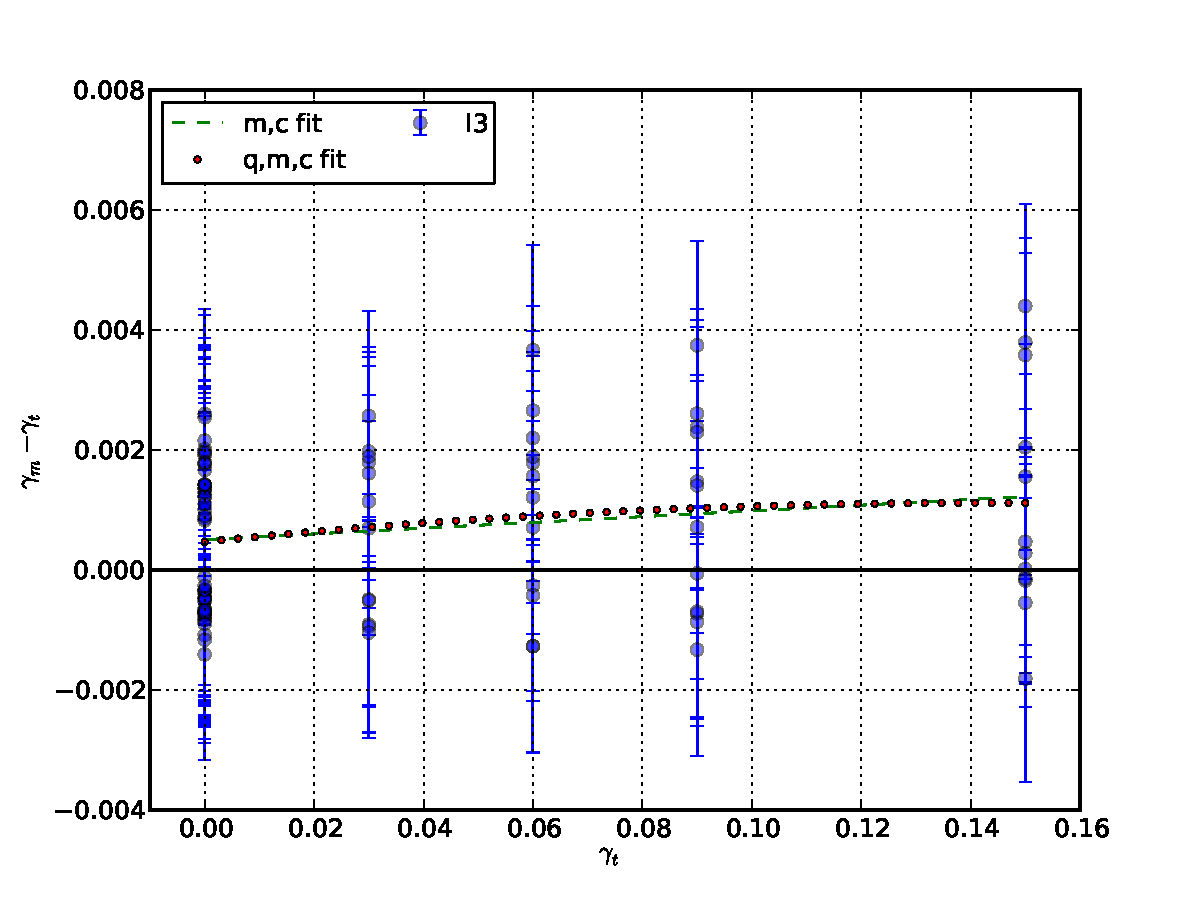
\includegraphics[width=0.45\textwidth]{fig/fitplt.pdf} 
  \caption{An example of the two types of fit used to quantify shape
    measurement error for the shear as measured by the im3shape
    pipeline (I3) on galaxy objects with Signal
    to Noise Ratio greater than 50. \green{show an example with more significant difference between the two fits; use larger labels} }
\label{fig:eqfit}
\end{figure}

%%%%%%%%%%%%%%%%%%%%%%%%%% Details on the sims (goes into Sec 2: CStep Challenge)
\begin{figure}
 \centering  % this centres figure in column
  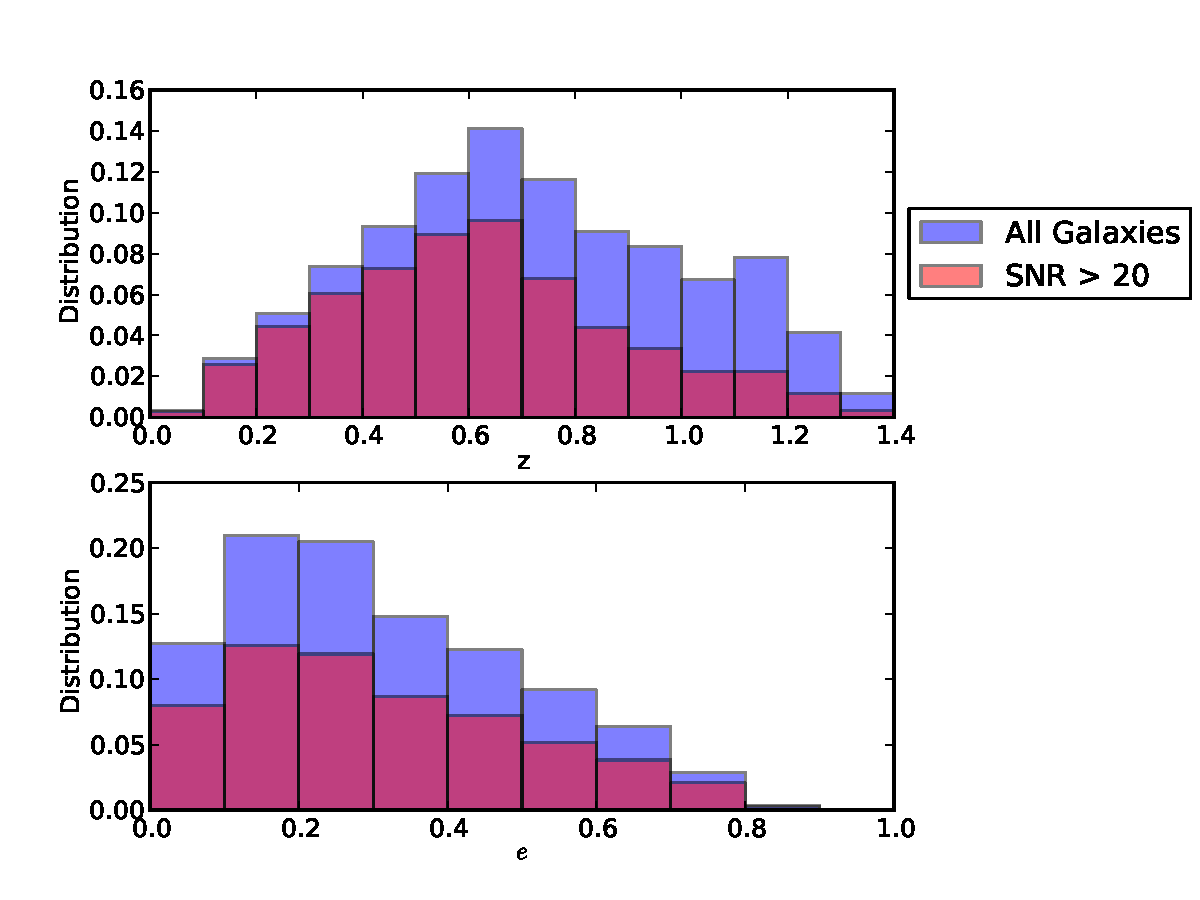
\includegraphics[width=0.45\textwidth]{fig/Out_hist_v2_truth.pdf} 
  \caption{Distributions of various galaxy 
properties in the CSTEP simulation. The top plot shows the
redshift distribution of galaxies as a function of percentage in the simulation. 
The bottom plot shows the distribution of intrinsic ellipticity as a
function of percentage of total objects. The
total number of galaxy objects included is 141559 and is shown in blue, the number of
galaxy obejects with SNR $>$ 20 is 84586 and is shown in magenta.}
\label{fig:Galprop}
\end{figure}
The image simulations used in the CSTEP project were designed to 
replicate the properties of the final co-added data that will be taken by the 
Dark Energy Survey. The Dark Energy survey is an optical survey of
5000 deg$^2$ of the southern sky, that will image around 300 million
galaxies in five filters (g,r,i,z and Y) \citep{Klaus}. To test the DES
data management system and software pipelines developed by the 
science working groups detailed image simulations were created by the 
DES Simulation team \citep{DESsim}. Each simulated image used in CSTEP models the DES focal plane
with 62 CCDs each of which is 2K x 4K pixel (0.27''/pixel). Star and galaxy objects are
rendered by drawing random samples of
photons from the theoretical light profile of the source convolved 
by the PSF. \\
\indent For the CSTEP simulated images, mock galaxy catalogs were
created with the ADDGALS  method that reproduce observed correlations
for galaxies among clustering, luminosities, and colors. 
The parent N-body simulations used by ADDGALS are the ``Carmen'' Las Damas
N-body simulation box (1 Gpc/$H^3$ ) with  $ \Lambda$ cosmology, $\Omega_M
= 0.25, \sigma_8 = 0.8$, at $z< 1.35 $
(\cite{LasDamas}). In each image around $ 140,000 $ galaxy objects are
present. The simulated galaxy images are designed to have similar properties to
the galaxies that DES will observe by combining a mock
catalog with empirical data from the HST/GEMS catalog for galaxies
with magnitude r $ > $ 23 , and from the SDSS for
galaxies with magnitude r $ < $ 23. The distributions of galaxy
properties in the simulation are shown in Figure \ref{fig:Galprop}. 
The galaxy objects are created with Sersic profiles with an
index that ranges from 0.5 to 5.  \\
\indent The CSTEP simulated images contain a constant
PSF which eliminates the technical challenge of determining the best
way to model a varying PSF. For CSTEP there are two
branches in the image simulation sets, those that include a circular
Gaussian PSF and those that include an elliptical Gaussian PSF. 
The elliptical Gaussian PSF has $ \epsilon =
0.03 $. For both the Gaussian and elliptical Gaussian
PSF the simulated images contain a convolution kernel that mimics the
range of isotropic distortion due to the atmosphere that DES will
likely observe. This isotropic distortion simulates seeing conditions,
or atmospheric blurring, of $ 0.7 - 0.9 $ arcsec. 
A summary of the PSF image properties is included in Table \ref{table:tab2}. 
For each PSF there are 8 focal plane images that contain constant
shear for $\gamma = 0.0$ to $\gamma = 0.15$ in both
$\gamma_1$ and $\gamma_2$, as described in Table \ref{table:tab2}.  
\begin{table}
\begin{centering}
\begin{tabular}{ccc}
\hline
PSF Number & Type & Seeing  \\
\hline
1 & circular Gaussian & 0.7 \\
2 & circular Gaussian & 0.8 \\
3 & circular Gaussian & 0.9 \\
4 & elliptical Gaussian & 0.75 \\
5 & elliptical Gaussian & 0.8  \\
6 & elliptical Gaussian & 0.9  \\
\hline
\hline
Shear Number & $ \gamma_1 $ & $ \gamma_2 $  \\
\hline
1 &  0.0 & 0.03 \\
2 &  0.0 & 0.06 \\
3 &  0.0 & 0.09 \\
4 &  0.0 & 0.15 \\
5 &  0.03 & 0.0 \\
6 &  0.06 & 0.0 \\
7 &  0.09 & 0.0 \\
8 &  0.15 & 0.0 \\
\hline
\end{tabular}
\end{centering}
\caption{ Summary of the PSF and shear sets for the CSTEP simulated images. }
\label{table:tab2}
\end{table}



%%%%%%%%%%%%%%%%%%%%%%%%%%%%%%%%%%%%%%%%%%%%%%%%%%%%%%%%% Sec 3
\section{Shape measurement pipelines}
There are eight weak lensing pipelines that submitted 
results for the CSTEP project, shown in Table \ref{table:smp}.
There are several lensing pipelines tested in this challenge that could potentially
be used to create shear catalogs for DES. These implementations
represent a broad range of lensing pipeline types, and can be divided
into four groups. Methods are grouped using roughly the same criteria 
as in STEP2 \citep{STEP2}. A short description of the methods is
included below with a detailed pipeline description included in
Appendix \ref{App:shpipe}.\\

\subsection{Red class methods}
The red class methods (DE, IM, PK, KM) are based on the oldest 
shape measurement method KSB+ developed by 
\citet{KSB}. As in STEP2, red class methods are
defined as those that measure combinations of
moments of each galaxy image $I(x)$ using a Gaussian 
weighting function. Various implementations
of this class of methods have been studied in previous shape
measurement challenges, and the accuracy has been shown 
to vary widely \citep{STEP2, GREAT10}.  Two of the red class lensing
pipeline implementations included in CSTEP have performed well on
previous image simulations challenges (DE, KM). Other 
red class implementations that were calibrated on
simulated image data have been used in several recent 
weak lensing analyses\citep[e.g.][]{Gruen_s, Apple, TS}. Many of the
large weak lensing cluster studies have used red class
methods \citep{HH}, and KSB+ methods are the most common
method used to measure the mass of clusters using weak lensing.
 
\subsection{Green class methods}
The green class methods (GM, I3) are commonly known as model fitting
methods. These methods convolve various models of galaxies with different 
parameterizations, including their intrinsic shape, with the PSF and
determine those that best fit the galaxy image. The green class methods
\textsc{lensfit} and \textsc{DeepZot} were among the best performing 
methods in GREAT08 and GREAT10, and im3shape has been shown 
to perform well on the GREAT08 and GREAT10 data \citep{Jzun}. 
A green class method \textsc{lensfit}, was 
the lensing pipeline for the Canada-France-Hawaii 
Telescope Lensing Survey (CFHTLenS) \citep{CHey}. This catalog 
was then used for several scientific analyses, \citep[e.g.][]{CH1,
  CH2, CH3}. 

\subsection{Blue class methods}
The blue class methods (MJ) are methods which model the
galaxy images as a sum of orthonormal Gauss-Laguerre polynomial
functions, commonly known as \textsc{shapelets}. The MJ
method competed in the STEP1, STEP2, and GREAT08 challenge. 


\subsection{Purple class methods}
The purple class is used to describe a method significantly different from the
three main approaches outlined above, Fourier Domain Null Testing (FDNT,
\citealt{Bern}). In FDNT, the surface brightness profiles of PSF and
observed galaxy are transformed to Fourier space, where the latter is
de-convolved by dividing by the former. Testing the Fourier
representation of the galaxy for roundness after applying an inverse
shear, a likelihood of shears is determined. The information used in
the roundness test is limited to frequencies below those rendered
infinitely noisy by the PSF. FDNT is known to perform very well on low
noise simulations \citep{Bern} but has not been applied yet to
observed data for a scientific analysis.
 
\begin{table}
\begin{center}
  \begin{tabular}{| c | c | c| c | }
    \hline 
     Method & Key & Contributor & Class \\
    \hline
     DEIMOS & DE &  P. Melchior & Red  \\
    \hline
    IMCAT & IM & J. Young & Red  \\
    \hline
    ksbm &  KM & P. Melchior &  Red \\
    \hline
    PKSB & PK & D. Gruen & Red \\
    \hline
     Gaussian Mixtures & GM & E. Sheldon & Green \\
    \hline
     im3shape &  I3 &  B. Rowe & Green \\
    \hline
     Bernstein and Jarvis (2002) & MJ &  M. Jarvis & Blue \\
    \hline
     PFDNT &  PF & D. Gruen & Purple \\
    \hline
  \end{tabular}
\end{center}
\caption{ A summary of the lensing pipelines used to analyze CSTEP simulated images. }
\label{table:smp}
\end{table}



%%%%%%%%%%%%%%%%%%%%%%%%%%%%%%%%%%%%%%%%%%%%%%%%%%%%%%%%% Sec 4
\section{Evaluation of pipelines}
In this section we evaluate the performance of shape measurement 
pipelines based on a set of criteria important for large cluster weak
lensing studies. The success of a shape measurement pipeline depends
on its ability to accurately measure shear on small faint galaxies, be unbiased
when all galaxies present in an image are used to measure the shear, and
have a shear bias that does not change as a function of the redshift
of the galaxies included in the lensing measurement. A good shape
measurement method would also be able to successfully measure shear on
a high percentage of the galaxy images which it attempts to analyze. 
The relative importance of the above criteria in determining
the best shear measurement pipeline to use may depend both on the 
data being evaluated and the lensing application. A more detailed examination
of the performance of each individual lensing pipeline 
as a function of PSF ellipticity, PSF size, galaxy size, 
and the contribution of selection bias is included in Appendix \ref{App:shpipe}, along
with a description of the algorithms of the shape measurement pipelines. \\

The measure of signal-to-noise ratio (SNR) referred to in this section was measured on the CSTEP images
for each galaxy using \textsc{SExtractor}. It is defined as 
\begin{equation}\label{Eqn:SNR_ref}
\textrm{SNR} = \frac{\textrm{Flux}}{\textrm{Flux Error}} \; ,
\end{equation}
where the flux and flux error was determined using ... \green{say FLUX\_AUTO or FLUX\_ISO here and give details on detection threshold in case it's the latter; I don't think the figure adds much since the MJ and I3 definitions of SNR are less common than this one, so I've removed it}.

\green{can you comment here or elsewhere on how you get the error bars on q,m,c? you should probably also mention how you fit for q,m,c (subtracting the mean intrinsic ellipticity of all galaxies as far as I remember, rather than doing a ring-test type thing)}

\subsection{Mean shape measurement bias}
In this section we include the average shape measurement 
bias results on a representative DES lensing catalog of 
all sources SNR $>$ 20. Most previous weak lensing studies 
rejected all objects below a set SNR threshold, but the 
depth chosen varies as it is determined by both the capabilities 
of the lensing pipeline used and the type of lensing analysis sought. In 
the CFHTLens survey all objects were rejected that were
measured as i'(AB) $<$ 24.7, or a SNR limit of around 10
\citep{cfhtls}. This limit was imposed for the CFHTLenS
catalog as it was the depth determined at which the 
photometric redshifts and shape measurements were too
poorly measured \citep{Hild}. For the CSTEP project
we chose objects SNR $>$ 20 for the representative DES 
lensing catalog. This is a conservative choice, and 
with additional lensing pipeline development a lower
SNR threshold could be chosen for the final DES 
lensing catalog. \\
\indent The average shape measurement bias on all images 
in the CSTEP simulations for galaxies SNR $>$ 20
is shown in Figure \ref{fig:QMC}. 
\begin{figure}
 \centering  % this centres figure in column
  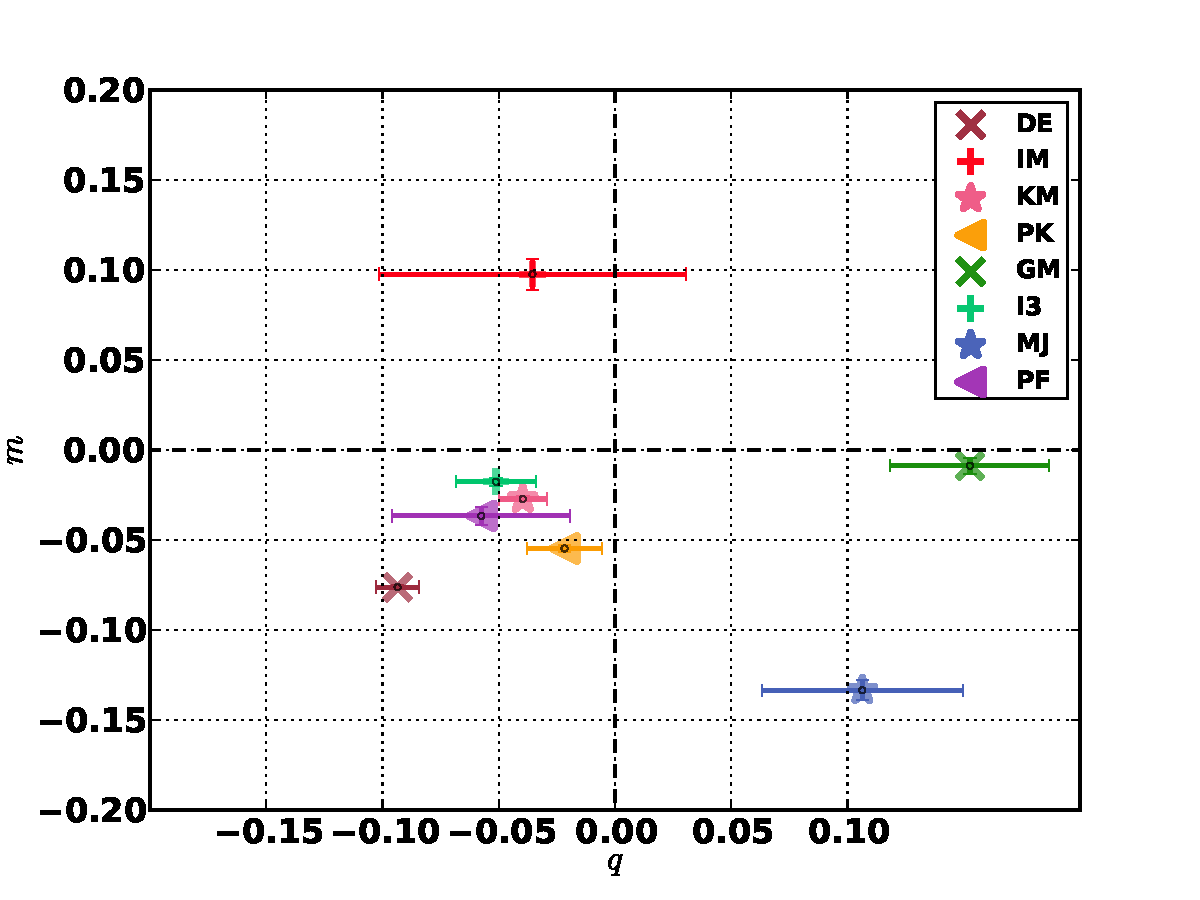
\includegraphics[width=0.45\textwidth]{fig/QMC_main_f.pdf} 
  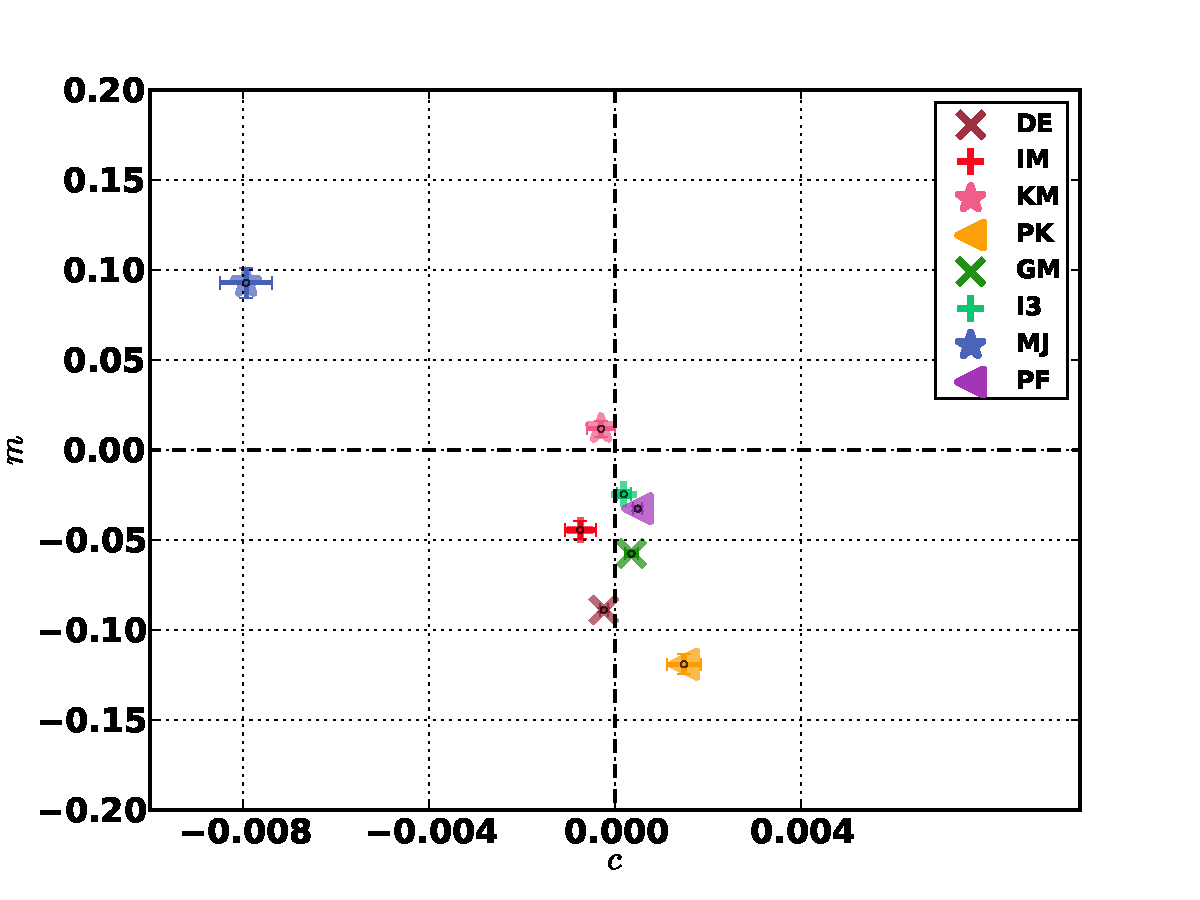
\includegraphics[width=0.45\textwidth]{fig/MC_main_f.pdf} 
  \caption{This figure shows the average shape measurement bias
as measured on all images for galaxy objects SNR $>$ 20. The
top panel shows the shape measurement bias $q$,$m$ as measured using 
a $q$,$m$,$c$ fit. The bottom panel shows the shape measurement bias 
$m$,$c$ as measured using a $m$,$c$ fit.}
\label{fig:QMC}
\end{figure}
Three of the lensing pipelines (I3, DE, KM) that are included in the
cluster STEP results, also competed in the GREAT10 challenge.
%The comparison between the GREAT10 and CSTEP results is shown in 
%Figure \ref{fig:gt10}. 
The results are roughly consistent between
the two challenges for I3 and KM showing that both pipelines are 
robust, and demonstrate similar levels of shape measurement bias
for a wide variety of sources and PSF types. Both I3 and KM are 
among the best performing lensing pipelines for both CSTEP and
GREAT10. 



\subsection{Quadratic shear bias}
In this section we discuss the importance of quadratic shape measurement 
bias on a representative DES lensing catalog of 
all sources with SNR $>$ 20. 

\green{added this interpretation:} As shown in the top panel of Fig.~\ref{fig:QMC}, quadratic biases of the pipelines tested in this work are at the level of or below $|q|\approx0.1$. Even at the larges shear tested ($\gamma_t=0.15$), this corresponds to a relatively minor bias compared to the typical level of multiplicative biases, i.e.~$|q|\gamma_t^2\ll|m|\gamma_t$. Quadratic biases are therefore a sub-dominant contribution to systematic errors in shape measurement for the pipelines tested. An exception may be the case of GM, which shows a small multiplicative but relatively large quadratic bias for the three-parameter fit.



\subsection{Dependence on galaxy signal-to-noise ratio}\label{sec:SNR}
\begin{figure}
 \centering  % this centres figure in column
  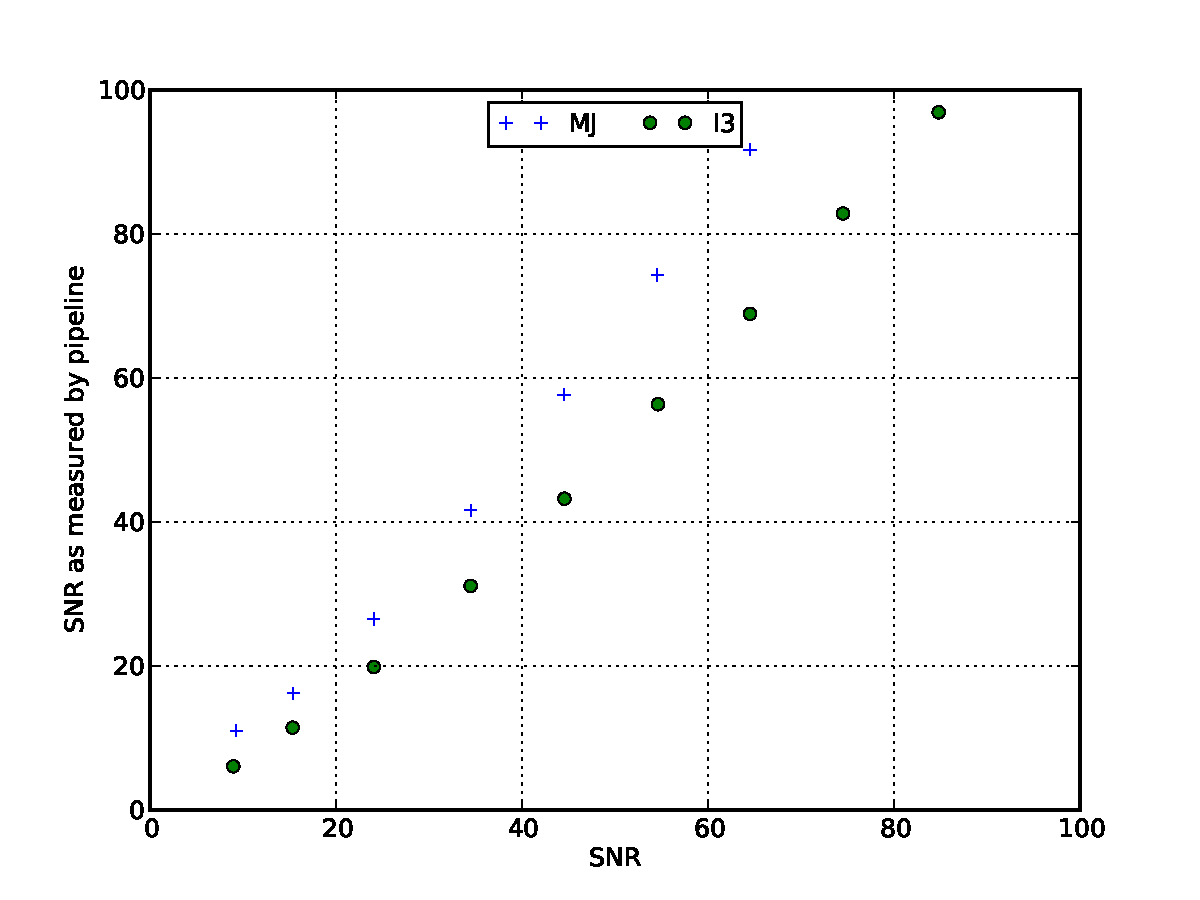
\includegraphics[width=0.5\textwidth]{fig/SNR_mfix.pdf} 
  \caption{The measurement of Signal-to-Noise Ratio (SNR) as defined
    in (cf Eqn.~\ref{Eqn:SNR_ref}) versus the SNR as measured by the
    individual pipelines.}
\label{fig:Snr_comp}
\end{figure}

The level of pixel noise present in galaxy images
greatly impacts the ability of lensing pipelines 
to accurately measure shear \citep[e.g.][]{peter_n, Okura_n, R_n}. 
The multiplicative bias due to pixel noise varies 
depending on both the source galaxy population
and the lensing pipeline. There have been a number
of calibration schemes that attempt to correct for the
effect of noise bias for specific lensing pipelines developed
including \citep{K_n} and \citep{cfhtls} on previous image 
simulations.  \\
\indent The Signal-to-Noise Ratio (SNR) was measured on the CSTEP images
for each galaxy using the Source Extractor software package 
\citep{Sext} with SNR defined as  
\begin{equation}\label{Eqn:SNR_ref}
SNR = \frac{\textrm{Flux}}{\textrm{Flux Error}}
\end{equation}
and where the flux was determined using automatic apertures.  A
comparision of the SNR as measured by Source Extractor and as measured
by the individual pipelines is shown in \ref{fig:Snr_comp}. 

To make the results easier to interpret and compare to previous
studies, the bias of the lensing pipelines was quantified in this
section by a linear function
\begin{equation}
\gamma_m = (m+1) (\gamma_t) + c
\end {equation}
where again $\gamma_t$ is the true shear and $\gamma_m$ is the measured shear.
The results of the multiplicative bias as a function of SNR are shown in Figure \ref{fig:Snr}. 
\begin{figure}
 \centering  % this centres figure in column
  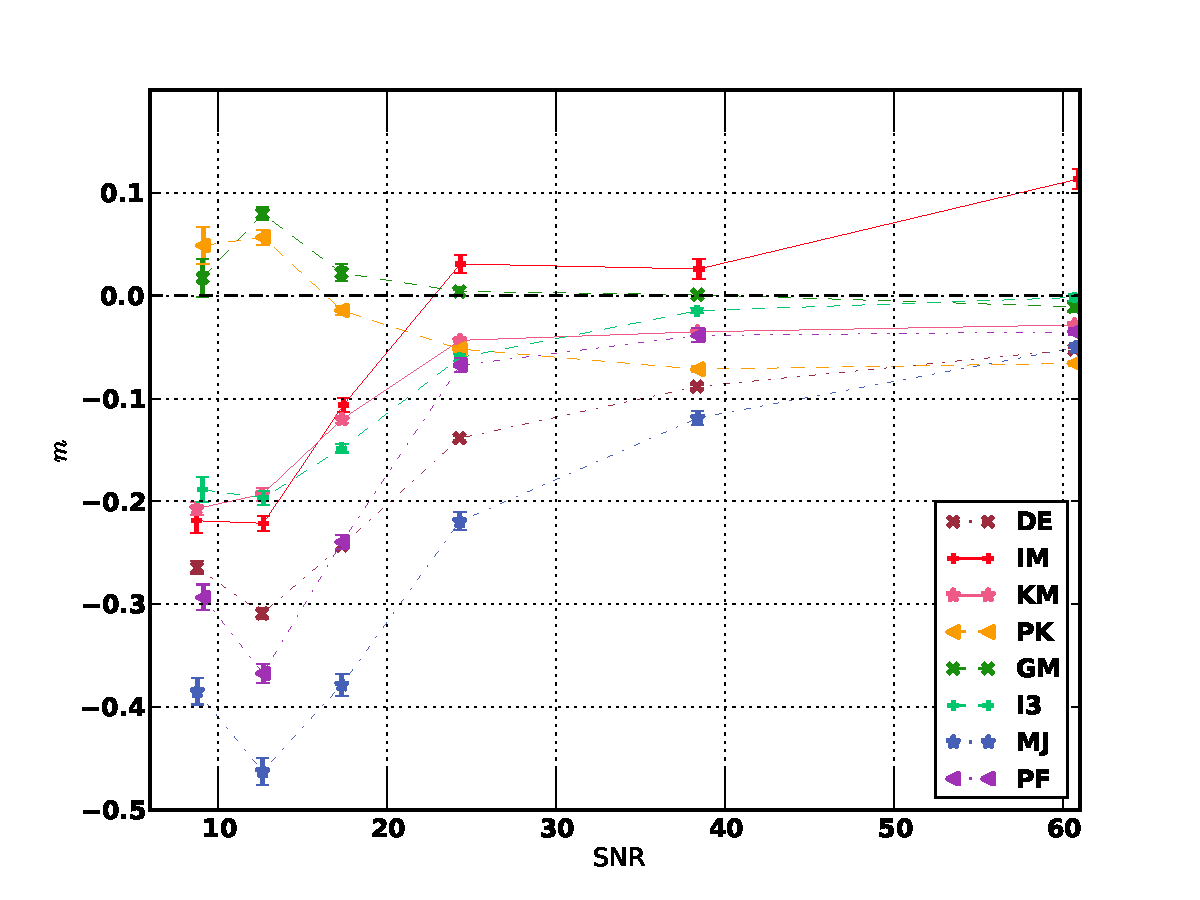
\includegraphics[width=0.5\textwidth]{fig/MvalSNR_v2.pdf} 
  \caption{Multiplicative bias ($m$) as a function
    of Signal-to-Noise Ratio (SNR). The multiplicative bias was determined
    using a linear fit of measured to true mean shear.}
\label{fig:Snr}
\end{figure}



\subsection{Selection effects and pipeline efficiency}
Lensing pipelines are not able to return 
a shear measurement for all galaxies in an
image. If a lensing pipelines preferentially rejects 
objects then the assumption that the population of galaxies used to
measure shear have $< \epsilon > = 0 $ may no longer be true. 
This selection bias effect has been discussed in STEP1 
where it was determined that results for some lensing pipelines  
improved when the non-zero mean intrinsic ellipticity of the surviving 
objects was corrected for. \\
\indent The fraction of successful shear measurements
 for each pipeline is shown for sources SNR $>$ 20 in Table \ref{table:sur_sel}.
The pipelines with the highest efficiency of successful measurements
are PK, DE and KM which are all moment based methods. 
As implemented in this challege the GM method
rejects a portion of the returned shear measurements and 
uses a weighting system in determining the average shear. Before the
flagged objects were rejected, the efficiency of GM was 0.93 and after
the efficiency was 0.24. The efficency of GM reported here is
therefore not directly comparable to the other lensing pipelines. 
\\
\indent
Pipelines may reject objects in a ellipticity dependent way. To test
for this selection effect bias, the $\gamma$ measured is corrected for
the intrinsic ellipticity of the sources as measured by each lensing
pipeline. I3 and DE do not appear to have a selection bias as their
accuracy is similar, before and after correction for $< \epsilon > \neq 0 $. The
pipeline that is most affected by selection bias is PF. Q, M and C as measured for each
lensing pipeline after correcting for selection effects is included in
Table \ref{table:QMC_sel} and Table \ref{table:MC_sel} . 
%%%%%%%%%%%%%%%%%% ************************
\begin{table}
        \centering
        \begin{tabular}{|c|c|c|c|c|c|c|c|}  
          \hline
          Pipeline  &  efficiency \\
          \hline
          DE &  0.92 \\
          \hline
          PF & 0.86 \\
          \hline
          GM & 0.24 (0.93) \\
          \hline
          MJ & 0.81 \\
          \hline
          PK & 0.90 \\
          \hline
          I3 &  0.79 \\
          \hline
          IM &  0.55 \\
          \hline
          KM & 0.91 \\
          \hline
        \end{tabular}
        \caption{The percentage survival of the shape measurement pipelines.}
    \label{table:sur_sel}
\end{table}



\begin{figure}
\centering
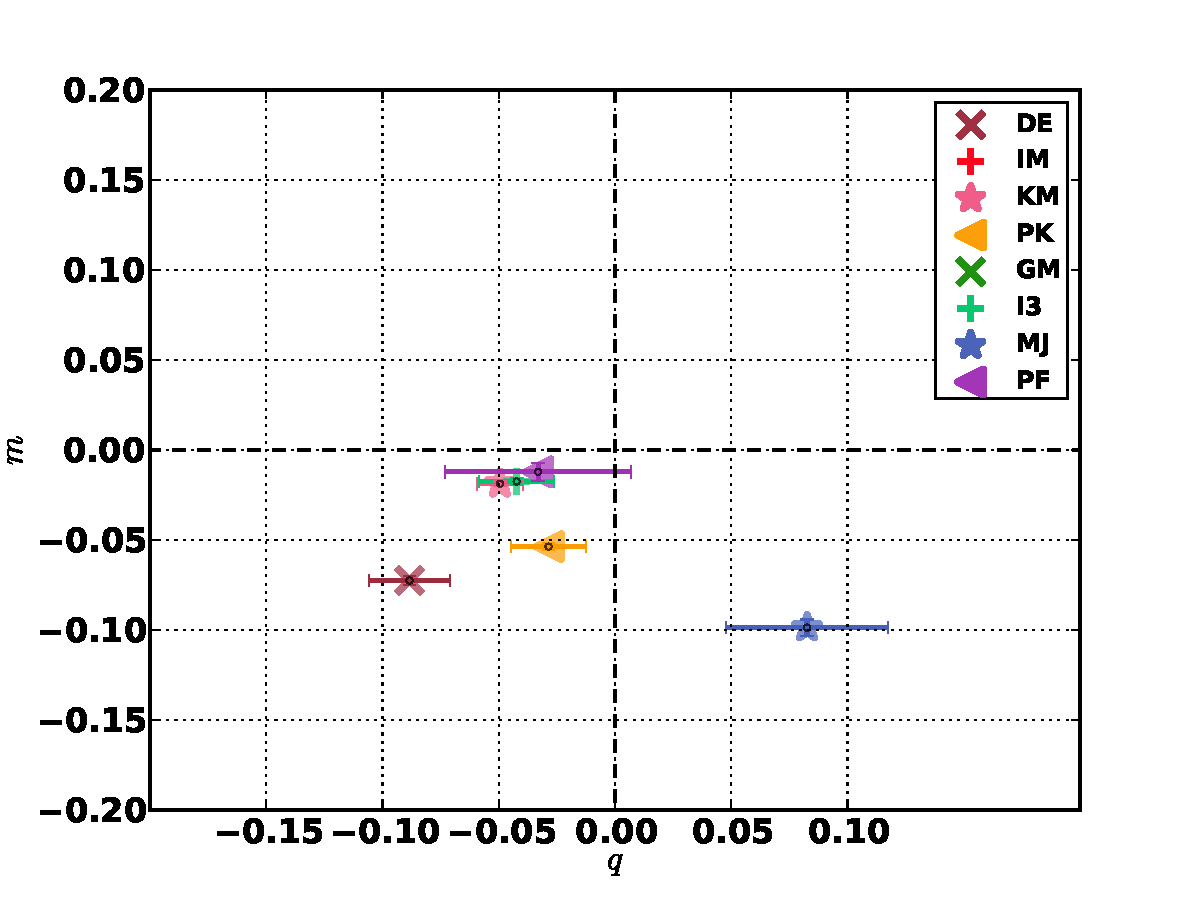
\includegraphics[width=0.5\textwidth]{fig/QMC_main_sel_f.pdf} \\
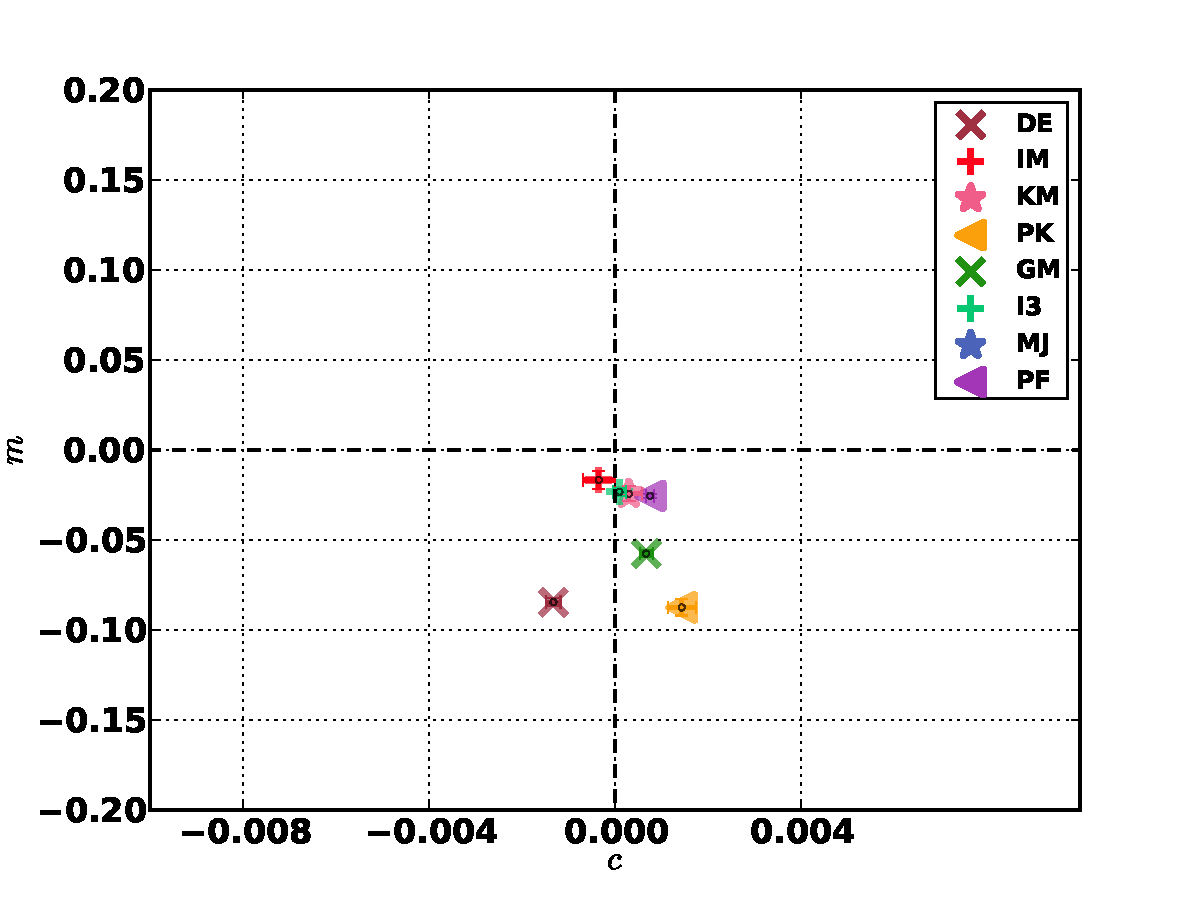
\includegraphics[width=0.5\textwidth]{fig/MC_main_sel_f.pdf} 
\caption{Average Q and M results for all pipelines for objects 
SNR $>$ 20 after correcting for selection effects in the top
panel and average M and C results for all pipelines
for objects SNR $>$ 20 in the bottom panel.}
\label{fig:QMC_main_sel}
\end{figure}



\subsection{Shape measurement bias as a function of redshift}
To ensure that the cosmology extracted using the
halo mass function as measured on galaxy clusters
using weak lensing is accurate, it is important that
galaxy clusters at various redshifts have 
similar levels of shape measurement bias. The population of 
galaxies observed at different redshifts will vary in
S/N, ellipticity distribution, size and morphology;
all properties which can affect the accuracy of a lensing 
measurement. The bias of galaxy sources with S/N $>$ 
20 as a function of redshift is shown in Figure \ref{fig:red}.
The results of bias of the lensing pipelines was quantified 
by fitting for M and C . 

\begin{figure}
 \centering  % this centres figure in column
  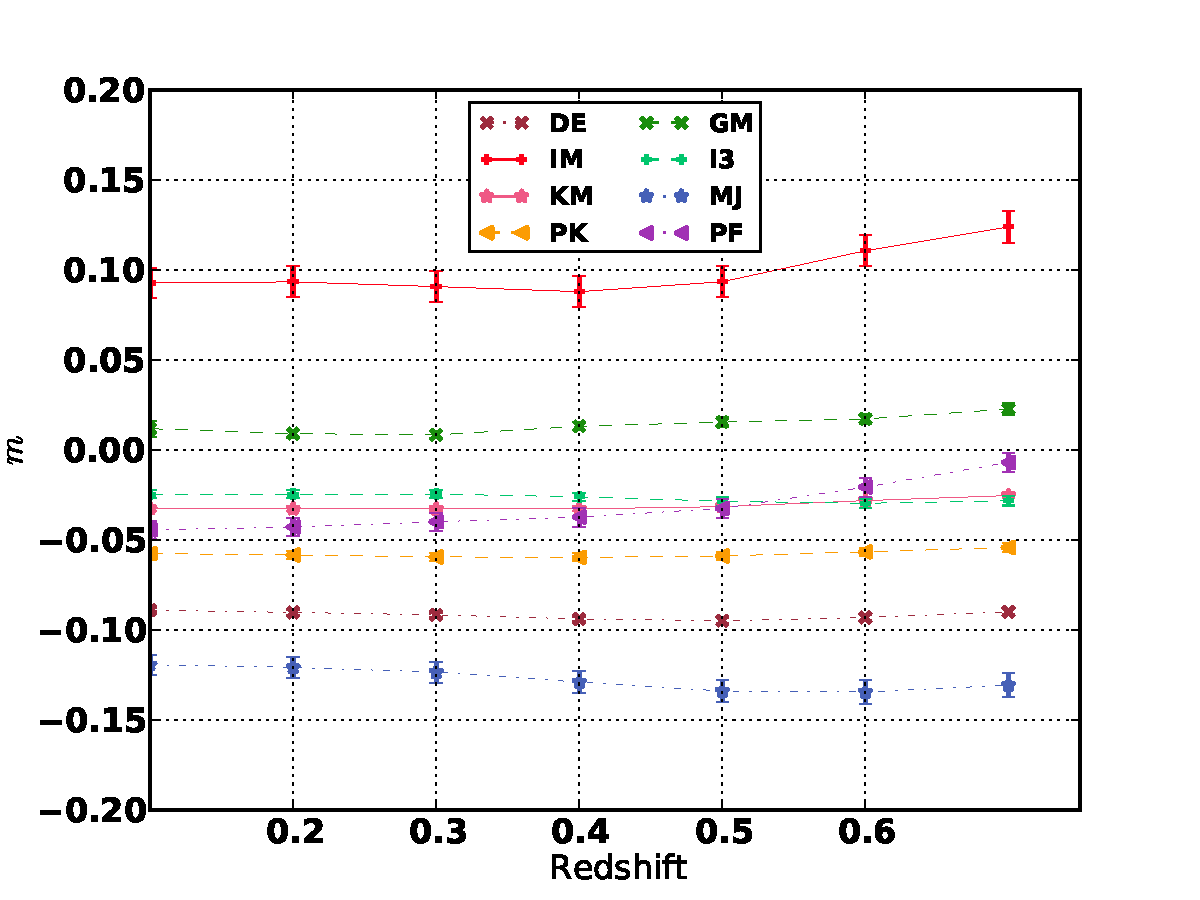
\includegraphics[width=0.45\textwidth]{fig/Mvalred_mfix.pdf} 
  \caption{Multiplicative shape measurement
  bias (M) of pipelines as a function of redshift.}
\label{fig:red}
\end{figure}
We find that MJ, DE, PK, I3 and KM
show a consistent level of shape measurement bias as a function of 
redshift. Our results are consistent with an analysis 
that studied the shape measurement bias as a function of redshift for I3 
\citep{K_2} on simulated COSMOS galaxies
and determined that it did not not vary significantly as a function
of redshift. 




\section{Stacked cluster weak lensing}
An accurate measurement of the abundance of galaxy clusters within a
given survey volume provides powerful constraints on cosmological
parameters.  While weak lensing can provide individual mass
measurements of high mass clusters, lower mass clusters can only be
measured on average by stacked weak lensing. Stacked weak lensing
measures the mean tangential shear of  background galaxies behind
galaxy clusters which are binned by an observable such as
richness. Stacked weak lensing
of clusters in the MaxBCG catalog \citep{Koester, Eshel} on data from the 
Sloan Digital Sky Survey \citep{York} has been used to derive
cosmological constraints on $\Omega_m$ and $\sigma_8$ in
\citep{Ying, ERozo}. Since ongoing and upcoming surveys such as DES  will provide deeper
imaging and better seeing over a wide area, the constraints on cosmology
from stacked cluster weak lensing will substantially improve if
sources of systematic error can be controlled.

There are a number of systematic effects that can bias the
stacked weak lensing mass measurement, including issues with background sample selection and redshift estimation like a contamination by cluster members, mis-centering of clusters, deviations of the fitted shear profile from the truth \citep[e.g.][]{mbecker}, orientation bias \citep{Joerg}, or a lack of full treatment of the intrinsic variation in cluster profiles \citep{ccv}. In this paper we focus
on the systematic bias in the stacked weak lensing cluster
mass measurement contributed by shape measurement. If lensing
pipelines provide a biased measurement of the shear profile of galaxy
clusters, this will bias the observed average cluster mass, and bias
the derived cluster abundance function. To model the possible
impact on a DES-like survey, we take the
average shear profile for each stacked cluster bin, apply a lensing
bias, and then determine what cluster mass would be measured. 
By comparing the true and the measured cluster
mass this provides an estimate of the effect of shape measurement bias
for each lensing pipeline. In this paper we compare the expected statistical errors
expected in a DES-like survey stacked weak lensing cluster mass measurement
described in section \ref{sec:p1} to the modeled bias on the mass
from shape measurement errors described in section \ref{sec:p2}.

\subsection{Stacked cluster weak lensing: statistical errors}\label{sec:p1}
Here we compare projected statistical errors of a DES like survey 
to systematic errors introduced by shape measurement bias on 
a simulated stacked cluster weak lensing
analysis. The distribution of cluster properties that we use is 
expected to be comperable to the distribution of clusters that will
be observed by DES. The statistical error we model for the stacked
cluster mass is dominated by shape noise in the background galaxies
and is modeled using the formula described in \citep{obscos, mbecker}.
\indent To create a simulated DES like stacked weak lensing survey we
take a simulated halo distribution, and then bin by mass and
redshift. For an analysis on observed data the clusters would
be binned by observables that are correlated with cluster mass such as richness,
optical luminosity, and X-ray luminosity. The different mass proxies used will
scatter some clusters into bins with a different median mass, but
will hopefully not greatly effect the average shear profile. In this
study we divide the cluster sample into four mass bins and six
redshift bins. The average mass, concentration, and redshift of the
clusters in each bin is determined and then used to calculate the
expected statistical error and an average NFW shear profile.  The
number of clusters in each mass bin and thier average redshift is
shown in Figure \ref{fig:N_Halo}. \\  
\indent To estimate the average redshift of background galaxies behind
each bin 
we use a redshift distribution of galaxies expected by a DES like survey
\begin{equation}
f(z) = z^m exp(-( z/z_* )^{\beta}) 
\end{equation}
where $m=2.0 $, $z_*=0.5$ and $\beta = 2.0 $ as described in
\citep{obscos}. The average redshift of sources selected behind each
stacked weak lensing bin is shown in in Table
\ref{table:NWF_1_b} and Table \ref{table:NWF_4_b}.
\indent
The statistical error or mass uncertainty $\Delta$ ln$(M)$ as
described in \citet{obscos} for stacked weak lensing is :
\begin{equation}
\Delta \rm{ln}(M) = \sqrt{ (\Delta  \rm{ln} (M_{s}))^2 +
(\sigma_{wl} )^2 }
\end{equation}
which combines the error due to the shape noise and the error due to
scatter based on clusters not being spherical. From \citep{mbecker}
we take
\begin{equation}
\sigma_{wl} = \frac{0.3}{\sqrt{N}}
\end{equation}
where N is the number of clusters in a given bin. To calculate the
shape noise we use the equation
\begin{equation}
\Delta \rm{ln} (M_{s}) = 6.0*10^3
(\frac{N}{N_{A}})^{0.5} (\frac{M}{M_{o}})^{-0.66} (\frac{\overline{ngal}}{N_{o}})^{-0.5}(\frac{D_{A}}{0.5})^{-1}
\end{equation}
from \citep{obscos} . To model the concentration we expect
for clusters at this redshift we assign an initial concentration c
\begin{equation}
c= A*( m_{200}/(2.0*1.e12))^{B}*(1 + z_{\rm{cluster}})^{C}
\end{equation}
Where  $ A = 7.85 $ ,  $ B = -0.081 $ , $ C= -0.71 $ and $m_{200}$ is
the mass within $r_{200}$ from \citep{oguri}.

\begin{figure}
 \centering  % this centres figure in column
  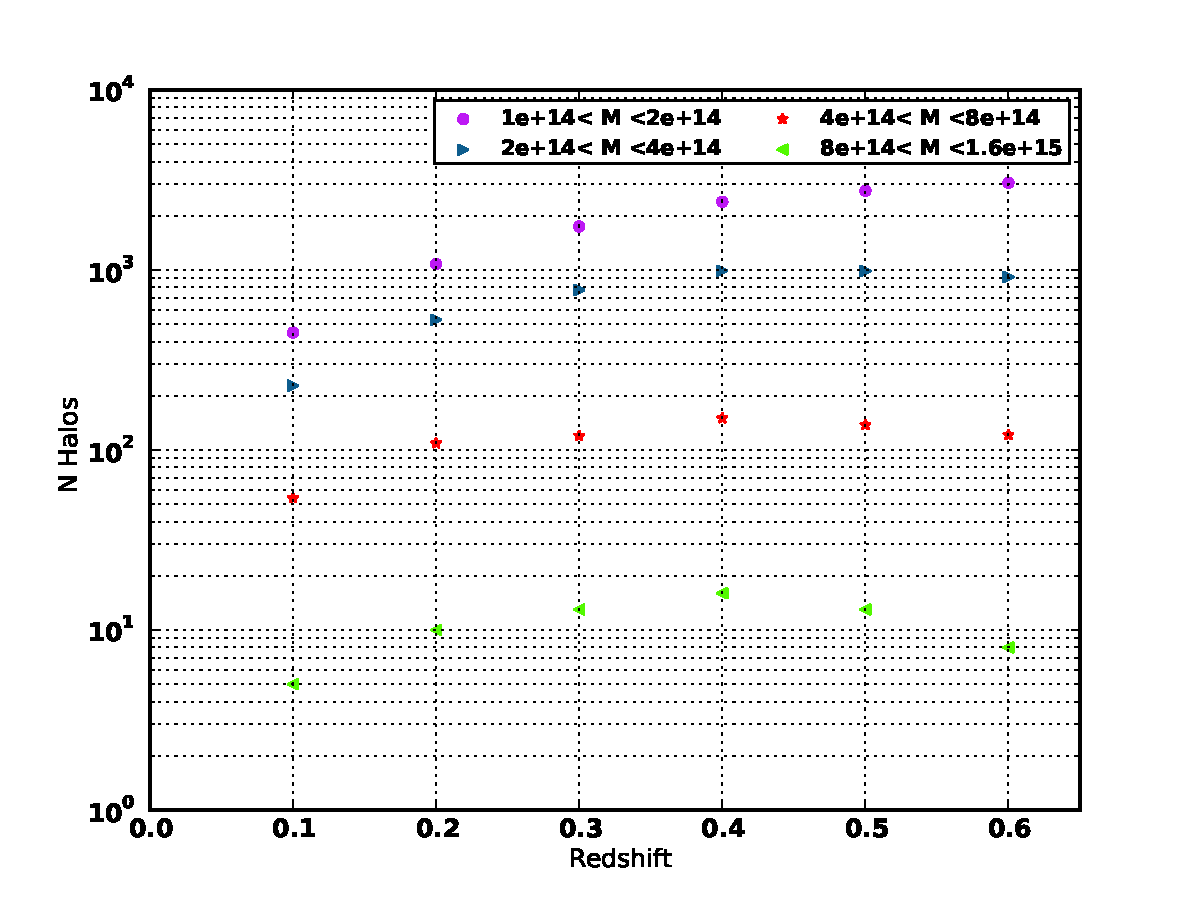
\includegraphics[width=0.55\textwidth]{fig/Halo_N.pdf} 
  \caption{The number of halos in each given mass bin.}
\label{fig:N_Halo}
\end{figure} 

\subsection{Stacked cluster weak lensing: modeled systematic errors}\label{sec:p2}
Here we model the systematic errors on the stacked cluster weak
lensing measurement by comparing the average mass in each bin
to the mass measured by a shear profile, affected by shape 
measurement bias. To measure the effect of shape measurement bias, a \citet*{1997ApJ...490..493N} (NFW) density profile is created for each mass bin. This density profile is
used to calculate the tangential reduced shear $g$ as described in \cite{NFW}. \\

\iffalse
\green{I don't think we need this}
\indent The NFW density profile is given by
\begin{equation}
\rho(r) = \frac{\delta_c\rho_c}{(r/r_s)(1+ r/r_s)^{2}}
\end{equation}
where $\rho_c = \frac{3 H^2 (z) }{8 \pi G} $ is the critical density , $
H(z) $ is Hubble's parameter , $G$ is Newton's constant, $r_s =
r_{200}/c$, $c$ is the concentration and 
\begin{equation}
\delta_c = \frac{200}{3}\frac{c^3}{ln(1+c) - c/(1+c)}
\end{equation}
from \citep{NFW} . The reduced shear from a NFW
halo is 
\begin{equation}
g = \frac{\gamma}{1-\kappa} = \frac{ \Delta \Sigma / \Sigma_c }{1
-\overline{\Sigma}/ \Sigma_c}
\end{equation}
\fi

The reduced shear as measured including shape bias is modeled as 
\begin{equation}
g' = (1+m)g + qg^2 \; .
\end{equation}
We then fit this $ g' $ distribution to get a $M_{200}$ and $ c $
value. \green{need more details here ... I guess sources uniformly distributed in area over some range in radius, maximum likelihood?}

\green{interpretation of results; note that even if the systematic offset is within the statistical uncertainties in each bin, all bins combinedly being measured low is a different story... at least need to discuss that}

\begin{figure*}
 \centering  % this centres figure in column
  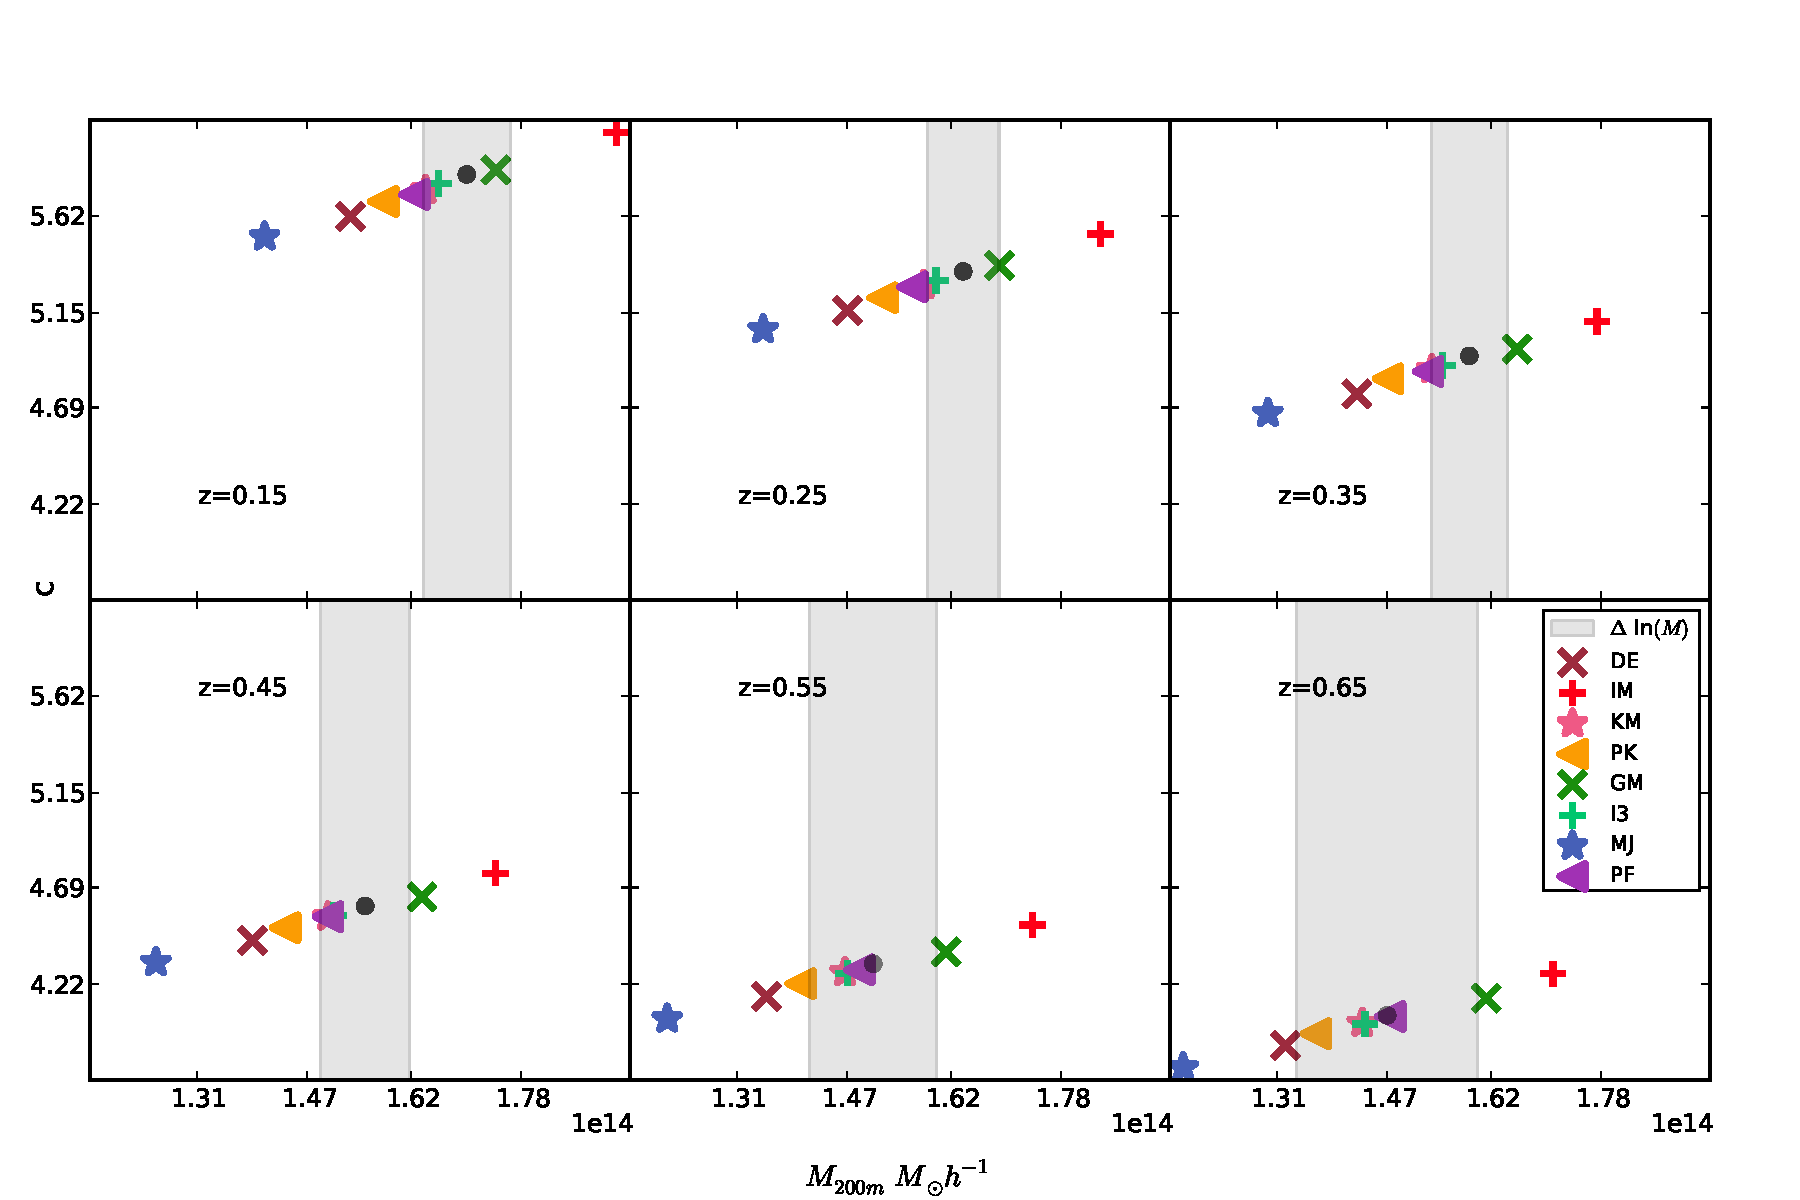
\includegraphics[width=0.95\textwidth]{fig/M_NFW_1.pdf} 
  \caption{NFW mass and concentration measured on a reduced shear
    profile affected by shape measurement bias
   as measured on all images for galaxy objects with SNR $>$ 20.}
\label{fig:M_NFW_1}
\end{figure*}

\begin{table*}
        \centering
        \begin{tabular}{|c|c|c|c|c|c|}  
          \hline
          N  &  $Z_{lens}$ & $Z_{source}$  & C & $M_{200m}$ $ M_\odot
          h^{-1}$  & $\Delta$ ln$(M)$ \\ 
          \hline
          450  & 0.16  & 0.58  & 5.82  & 1.70  & 0.037   \\
          \hline
          1080  & 0.26  & 0.62  & 5.35  & 1.64  & 0.032   \\
          \hline
          1744  & 0.35  & 0.66  & 4.94  & 1.59  & 0.035 \\
          \hline   
          2396  & 0.45  & 0.73  & 4.60  & 1.55  & 0.042   \\
          \hline
          2753  & 0.55  & 0.79  & 4.32  & 1.51  & 0.061   \\
          \hline
          3054  & 0.65  & 0.87  & 4.07  & 1.47  & 0.089   \\         
          \hline
        \end{tabular}
        \caption{ The expected statistical error due to one method of
          cluster stacking for a DES-like cluster distribution).}
    \label{table:NFW_1_b}
\end{table*}


\section{Summary}
The CSTEP project tested shape measurement pipelines in the cluster
shear regime on simulated data of DES. This project
analyzed the effectiveness of the shear pipelines by several criteria,
and tested the impact shape measurement bias would have on a stacked
cluster weak lensing analysis. \\

In this paper we measured Quadratic, Multiplicative and
Additive bias of galaxy shape estimates for eight shape measurement
pipelines. The shape measurement bias found in several of the pipelines was within the
desired limits of a stacked cluster weak lensing measurement for
DES. In particular the I3 pipeline has consistently good bias properties
across a wide range of simulation input parameters.\\

The results on the simulations showed that the strongest
determination of high bias was a low Signal to Noise Ratio (SNR). A
low signal to noise ratio occurs when the differentiation between
galaxy boundaries and their background is poor. In contrast, galaxies 
simulated at different redshifts had the same level of bias. An
important finding is based on an analysis of bias as a function of galaxy model
type. For many of the pipelines, and I3 in particular, galaxy
model type has little impact on measures of pipeline bias. \\

The results showed that in general the Quadratic bias was not
significant for most pipelines and that it did not contribute
significantly to the error in the mass measured on stacked cluster
weak lensing profiles. \\

This project has helped determine the properties of pipelines
to be used in DES. The use of the I3 pipeline
finds support by the consistently high quality of the shape
estimates. In addition, the characteristics of bias have been further
clarified, leaving in general bias as a multiplicative function
dominated by Signal to Noise ratio - leading to support of future
multiplicative corrections for Signal to Noise ratio in future
analysis. \\

 

 


\section*{Acknowledgments}
I thank......


%%%%%%%%%%%%%%%%%%%%%%%%%%%%%%%
%\let\jnl@style=\rm
%\def\ref@jnl#1{{\jnl@style#1}}

\def\aj{AJ}                   % Astronomical Journal
\def\araa{\ref@jnl{ARA\&A}}             % Annual Review of Astron and Astrophys
\def\apj{ApJ}                 % Astrophysical Journal
\def\apjl{ApJ}                % Astrophysical Journal, Letters
\def\aap{A\&A}                % Astronomy and Astrophysics
\def\aaps{A\&AS}              % Astronomy and Astrophysics, Supplement
\def\mnras{MNRAS}             % Monthly Notices of the RAS
\def\prd{Phys.~Rev.~D}       % Physical Review D
\let\astap=\aap
\let\apjlett=\apjl
\let\apjsupp=\apjs
\let\applopt=\ao
%%%%%%%%%%%%%%%%%%%%%%%%%%%%%%%

\bibliographystyle{mn2e}
\bibliography{CSTEP_j}

\appendix
\onecolumn

%\section{Shape Measurement Bias}
%Three of the lensing pipelines (I3, DE, KM) that are included in the
cluster STEP results, also competed in the GREAT10 challenge.
The comparison between the GREAT10 and CSTEP results is shown in 
Figure %\ref{fig:gt10}. The results are roughly consistent between
the two challenges for I3 and KM showing that both pipelines are 
robust, and demonstrate similar levels of shape measurement bias
for a wide variety of sources and PSF types. Both I3 and KM are 
among the best performing lensing pipelines for both CSTEP and
GREAT10. 

\begin{figure}
 \centering  % this centres figure in column
  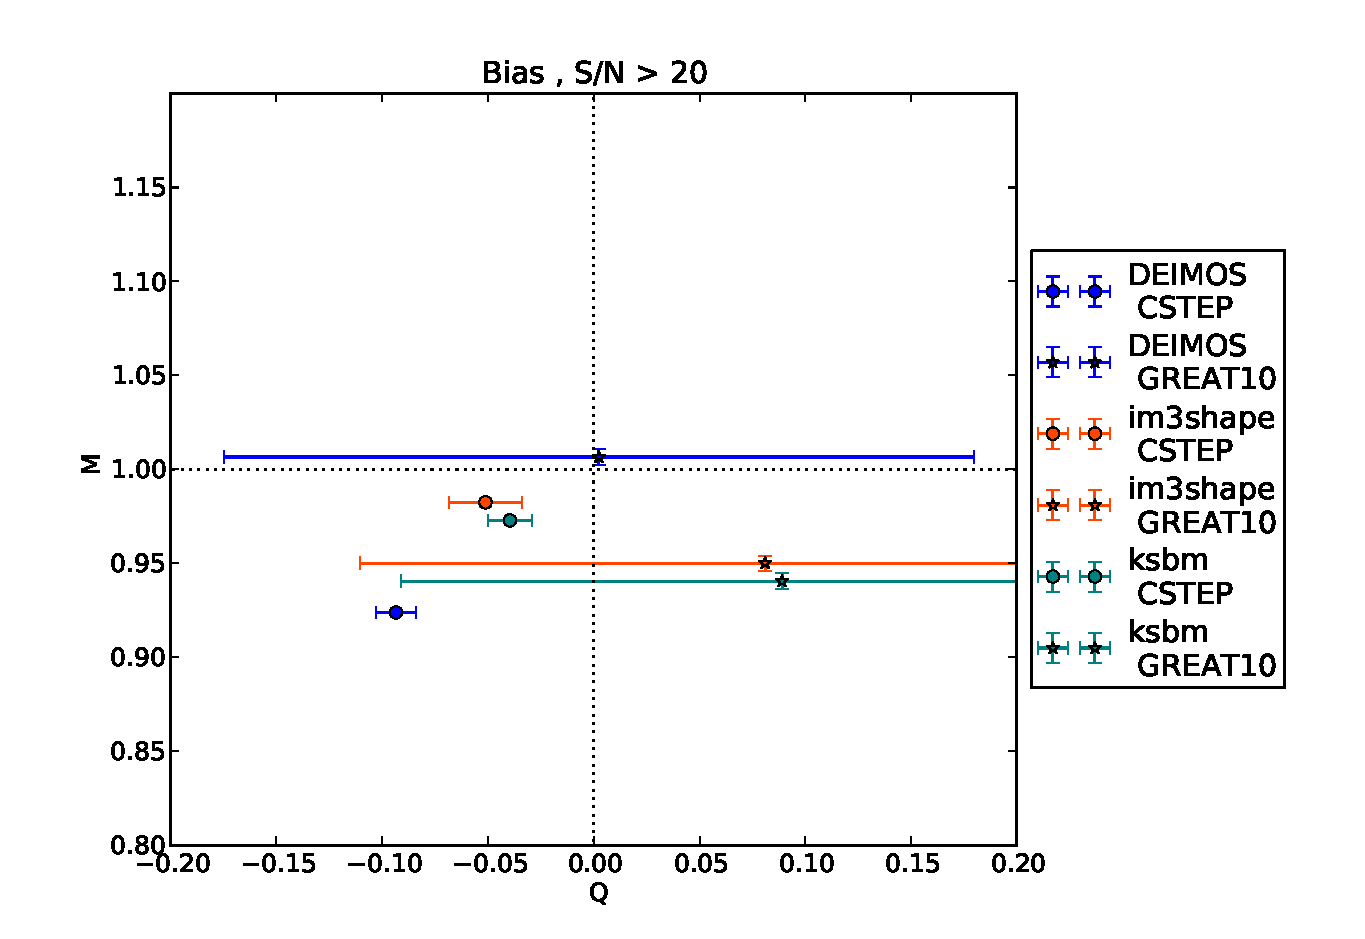
\includegraphics[width=0.45\textwidth]{fig/QMC_gt10.pdf} 
  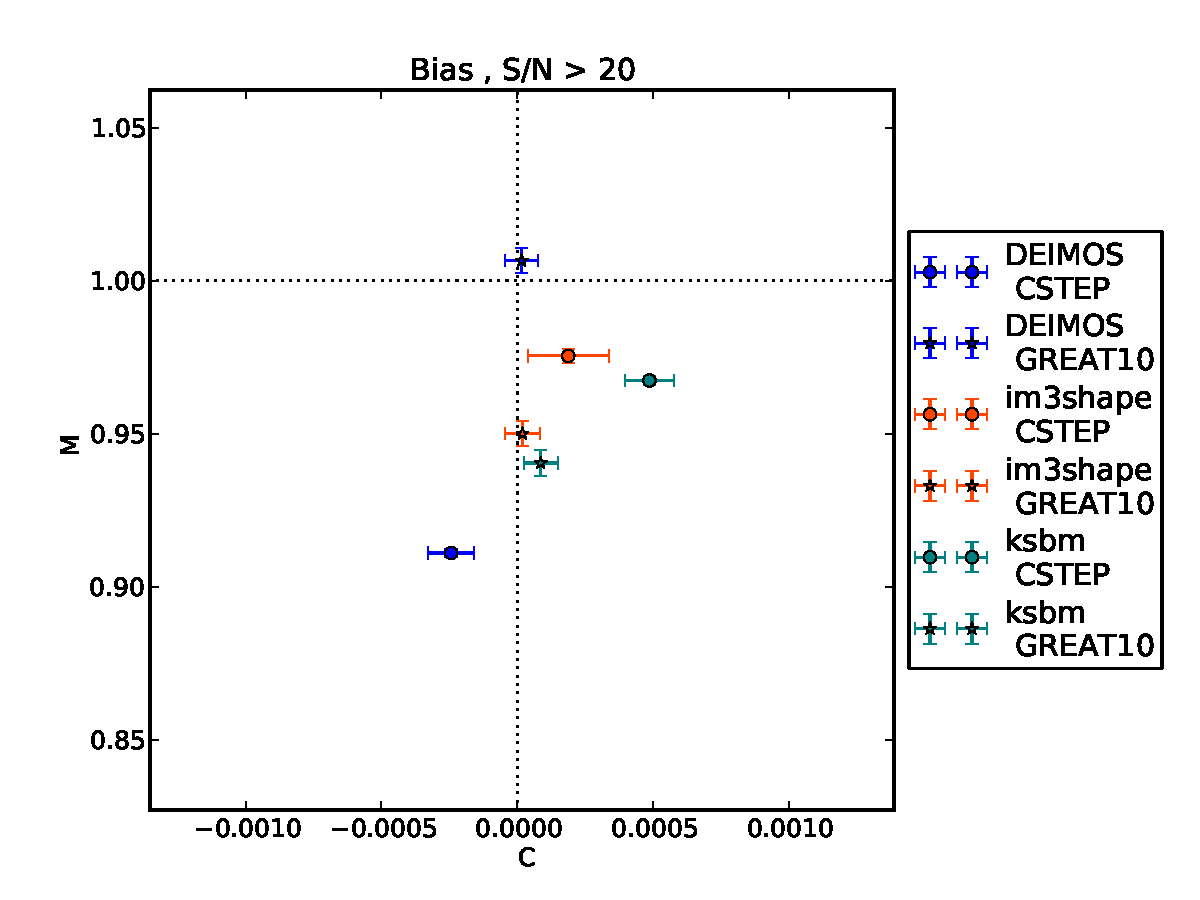
\includegraphics[width=0.45\textwidth]{fig/MC_gt10.pdf} 
  \caption{This figure shows the average shape measurement bias
as measured on all images for galaxy objects SNR $>$ 20 on
CSTEP data and the shape measurement bias as measured by the
same lensing pipelines on the GREAT10 data \citep{GREAT10}. The
top panel shows the shape measurement bias Q,M as measured using 
a Q,M,C fit. The bottom panel shows the shape measurement bias 
M,C as measured using a M,C fit.}
\label{fig:gt10}
\end{figure}

%%%%%%%%%%%%%%%%%%%%%%%%%%%%%%%%%%%%%%%%%%%%%%%%
\begin{table*}
        \centering
        \begin{tabular}{|c|c|c|c|c|c|c|c|}  
          \hline
          Pipeline & Qsel  & Msel  & Csel  & Q  & M  & C  \\
          \hline
          DE & -0.088 $\pm$ 0.017 & 0.928 $\pm$ 0.002 & -0.0014 $\pm$ 0.0002 & -0.094 $\pm$ 0.009 & 0.924 $\pm$ 0.001 & -0.0004 $\pm$ 0.0001 \\
          \hline
          PF & -0.033 $\pm$ 0.040 & 0.988 $\pm$ 0.005 & -0.0004
          $\pm$ 0.0003 & -0.058 $\pm$ 0.038 & 0.963 $\pm$ 0.005 &
          -0.0008 $\pm$ 0.0003 \\
          \hline
          GM & 0.236 $\pm$ 0.032 & 0.944 $\pm$ 0.004 & 0.0006
          $\pm$ 0.0003 & 0.153 $\pm$ 0.034 & 0.991 $\pm$ 0.004 &
          -0.0001 $\pm$ 0.0003  \\
          \hline
          MJ & 0.083 $\pm$ 0.035 & 0.901 $\pm$ 0.004 & 0.0015 $\pm$
          0.0003 & 0.106 $\pm$ 0.043 & 0.867 $\pm$ 0.006 & 0.0016
          $\pm$ 0.0004 & 0.81 \\
          \hline
          PK & -0.029 $\pm$ 0.016 & 0.946 $\pm$ 0.002 & 0.0006 $\pm$
          0.0001 & -0.022 $\pm$ 0.016 & 0.945 $\pm$ 0.002 & 0.0003
          $\pm$ 0.0001 \\
          \hline
          I3 & -0.042 $\pm$ 0.016 & 0.983 $\pm$ 0.002 & 0.0000
          $\pm$ 0.0001 & -0.051 $\pm$ 0.017 & 0.982 $\pm$ 0.002 &
          0.0001 $\pm$ 0.0002 \\
          \hline
          IM & -0.020 $\pm$ 0.058 & 1.275 $\pm$ 0.008 & -0.0066
          $\pm$ 0.0005 & -0.035 $\pm$ 0.066 & 1.098 $\pm$ 0.009 &
          -0.0080 $\pm$ 0.0006 \\
          \hline
          KM & -0.050 $\pm$ 0.010 & 0.981 $\pm$ 0.001 & 0.0007 $\pm$
          0.0001 & -0.040 $\pm$ 0.010 & 0.973 $\pm$ 0.001 & 0.0004
          $\pm$ \\
          \hline
        \end{tabular}
        \caption{ The Q, M, C results for objects SNR $>$ 20. The
          values reported are the reults of a Q,M,C fit after
          correcting for selection effects (Qsel, Msel, Csel) and not
          correcting for selection effects (Q, M, C).}
    \label{table:QMC_sel}
\end{table*}

\begin{table*}
        \centering
        \begin{tabular}{|c|c|c|c|c| }  
          \hline
          Pipeline & Msel  & Csel & M  & C   \\ 
          \hline
          DEIMOS & 0.915 $\pm$ 0.002 & -0.0013 $\pm$ 0.0002 & 0.911
          $\pm$ 0.001 & -0.0002 $\pm$ 0.0001 \\
          \hline
          PFDNT & 0.983 $\pm$ 0.005 & -0.0004 $\pm$ 0.0003 & 0.956
          $\pm$ 0.005 & -0.0007 $\pm$ 0.0003 \\
          \hline
          GaussianMix & 0.976 $\pm$ 0.004 & 0.0003 $\pm$ 0.0003 &
          1.012 $\pm$ 0.004 & -0.0003 $\pm$ 0.0003 \\
          \hline
          MJ & 0.913 $\pm$ 0.004 & 0.0014 $\pm$ 0.0003 & 0.881 $\pm$ 0.006 & 0.0015 $\pm$ 0.0004 \\
          \hline
          PKSB & 0.942 $\pm$ 0.002 & 0.0007 $\pm$ 0.0001 & 0.942 $\pm$
          0.002 & 0.0004 $\pm$ 0.0001 \\
          \hline
          im3shape & 0.977 $\pm$ 0.002 & 0.0001 $\pm$ 0.0001 & 0.975 $\pm$ 0.002 & 0.0002 $\pm$ 0.0002 \\
          \hline
          IMCAT & 1.272 $\pm$ 0.007 & -0.0066 $\pm$ 0.0005  & 1.093 $\pm$ 0.008 & -0.0079 $\pm$ 0.0006 \\
          \hline
          ksbm & 0.975 $\pm$ 0.001 & 0.0008 $\pm$ 0.0001 & 0.967 $\pm$ 0.001 & 0.0005 $\pm$ 0.0001 \\
          \hline
        \end{tabular}
        \caption{ The M, C results for objects SNR $>$ 20. The
          values reported are the reults of a M,C fit after
          correcting for selection effects (Msel, Csel) and not
          correcting for selection effects (M, C).}
    \label{table:MC_sel}
\end{table*}

%%%%%%%%%%%%%%% FIXX
%%%%%%%%%% !!!!!!!!
\section{Shear Measurement Pipelines}\label{App:shpipe}
\newpage 
\subsection{DEIMOS}
DEIMOS determines the shape of objects using the second
order moments of the light profile as measured by and elliptical
Gaussian weight function. In this challenge the DEIMOS pipeline eliminates objects with $ \gamma > 1.0 $
from the catalog. \\
 
\begin{figure*}
\centering
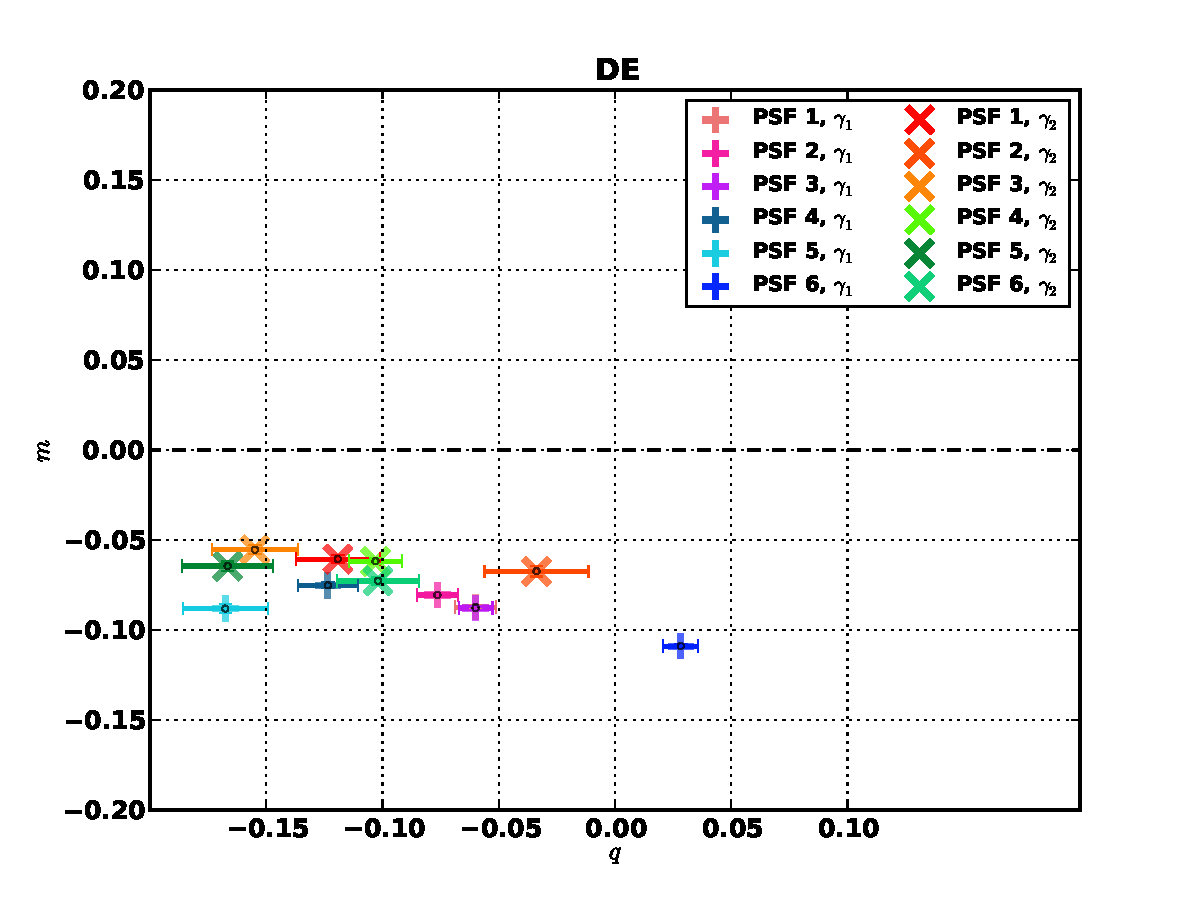
\includegraphics[width=0.45\textwidth]{fig/QMC_main_DE_f.pdf} 
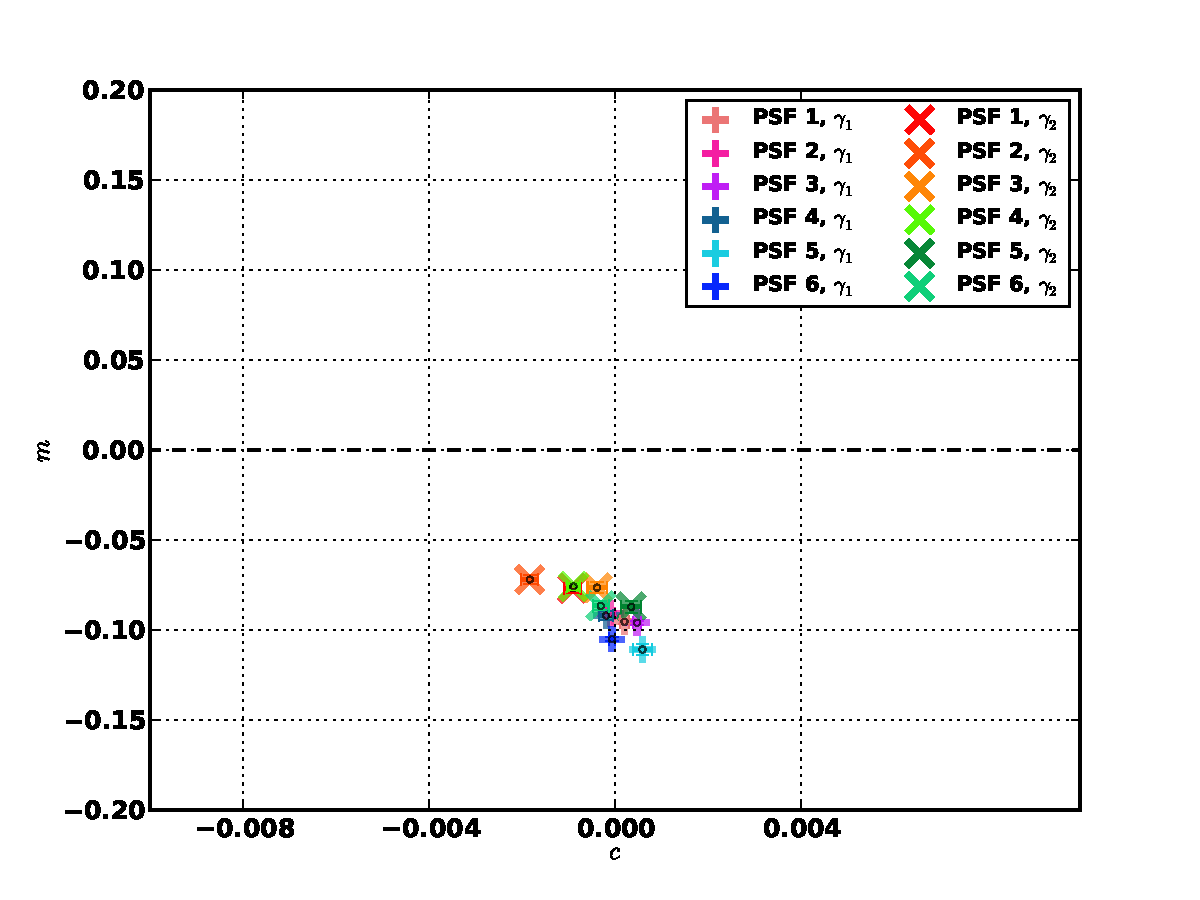
\includegraphics[width=0.45\textwidth]{fig/MC_main_DE_f.pdf} 
\caption{Average Q and M results for all pipelines for objects 
SNR $>$ 20 on the left and M and C results for all pipelines for objects 
SNR $>$ 20 on the right seperate by $\gamma_{1} $ and $\gamma_{2} $ as
well as PSF.}
\label{fig:DEIMOS_qmc}
\end{figure*}

\begin{figure*}
\centering
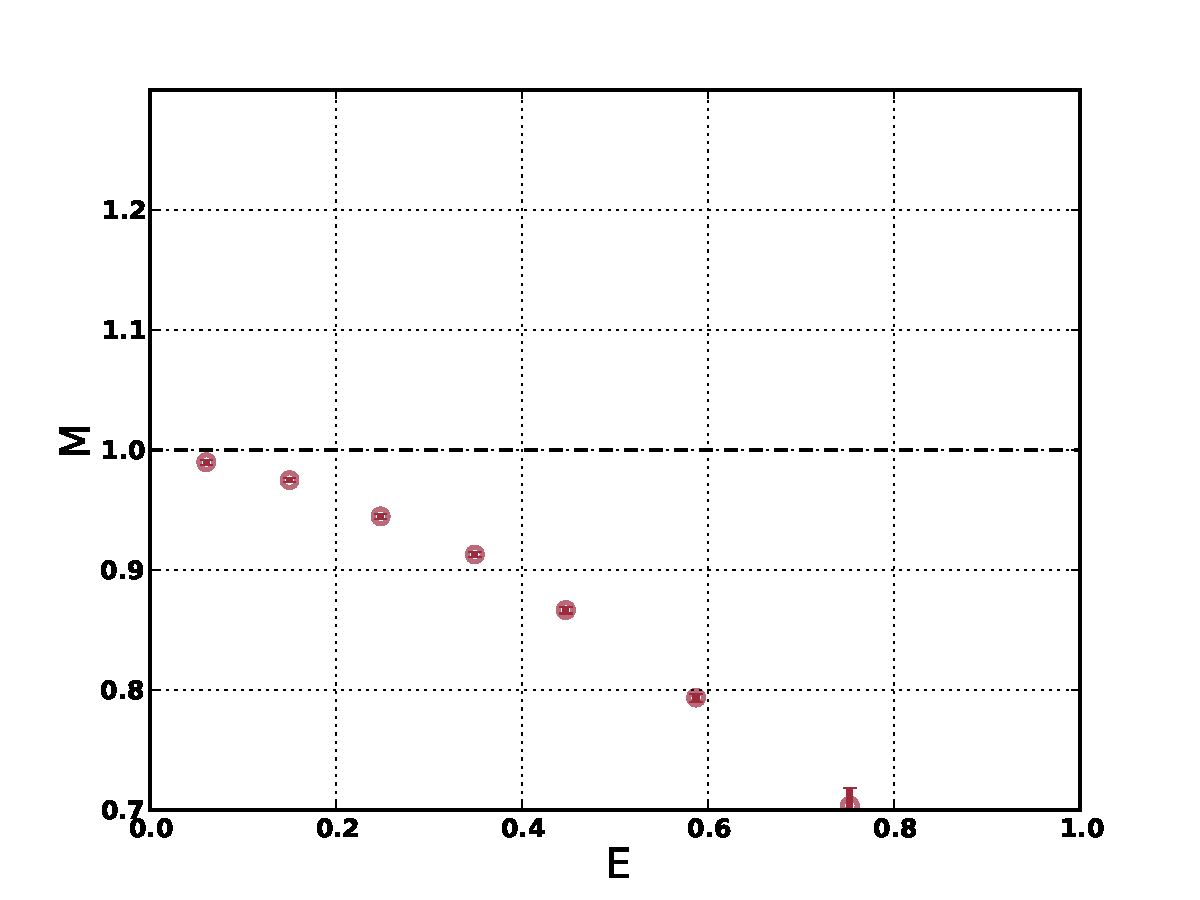
\includegraphics[width=0.45\textwidth]{fig/MvaleDE.pdf} 
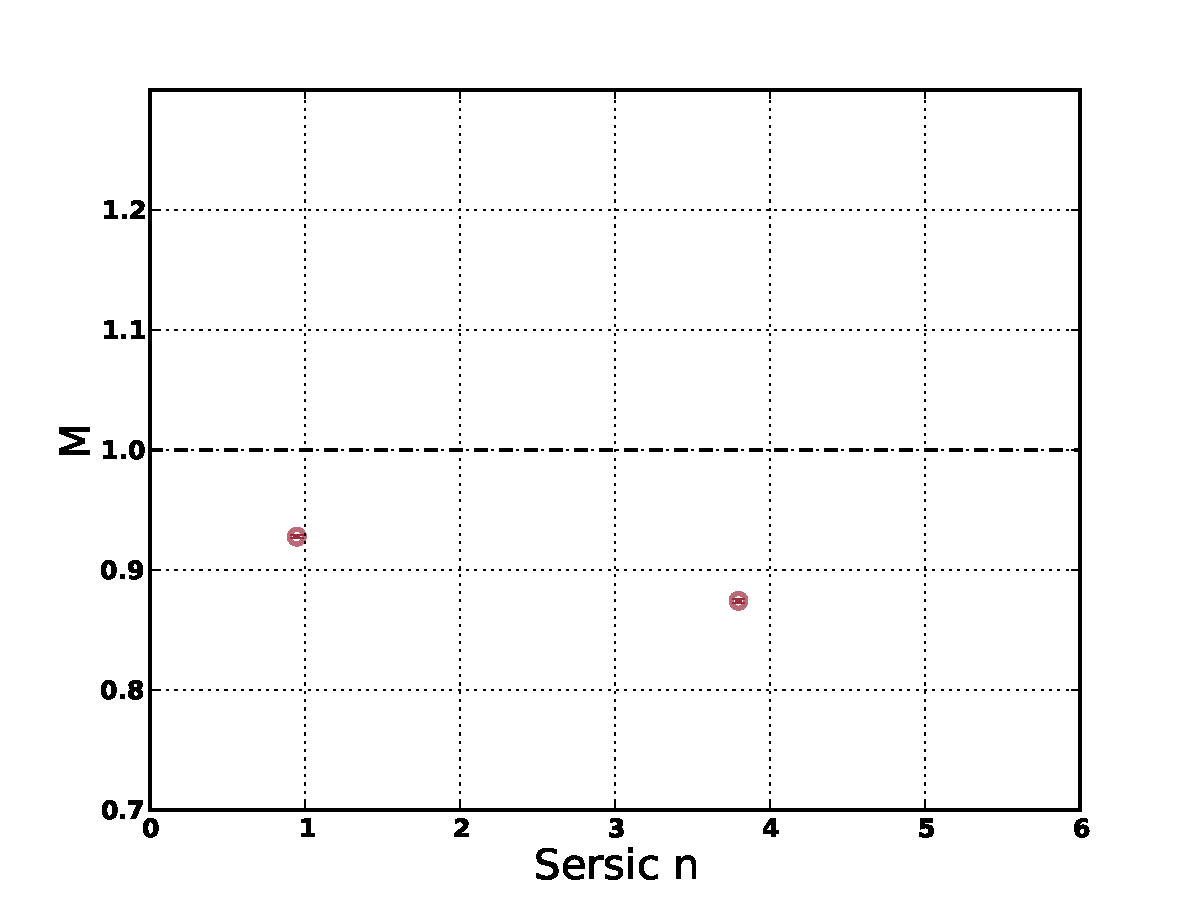
\includegraphics[width=0.45\textwidth]{fig/Mval_typeDE.pdf} 
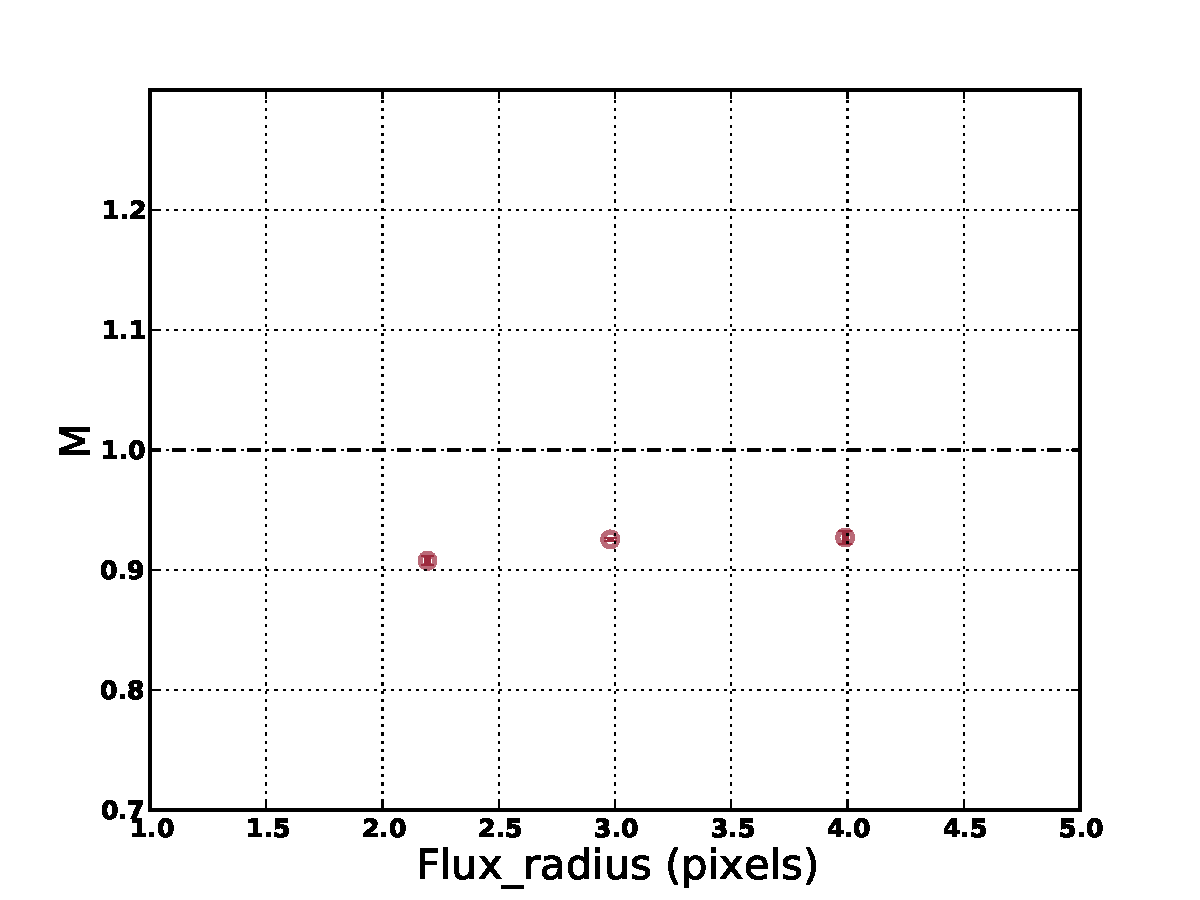
\includegraphics[width=0.45\textwidth]{fig/Mval_sizeDE.pdf} 
\caption{The M and C values for ...}
\label{fig:DEIMOS_m}
\end{figure*}

\newpage 
\subsection{IMCAT}
The KSB+ pipeline IMCAT measures the second order moments using an
elliptical gaussian. The implementation of IMCAT used on the CSTEP images
took an average of the $P^{sm}$ and $p^*$ of selected stars in the
image to calculate the PSF. The average of the trace of the two
matrices $P^{sm}$ and $P^{sh}$ were multiplied by the identity
matrix. The IMCAT pipeline eliminates objects with $ \gamma > 1.0 $
from the catalog.  \\

\begin{figure*}
\centering
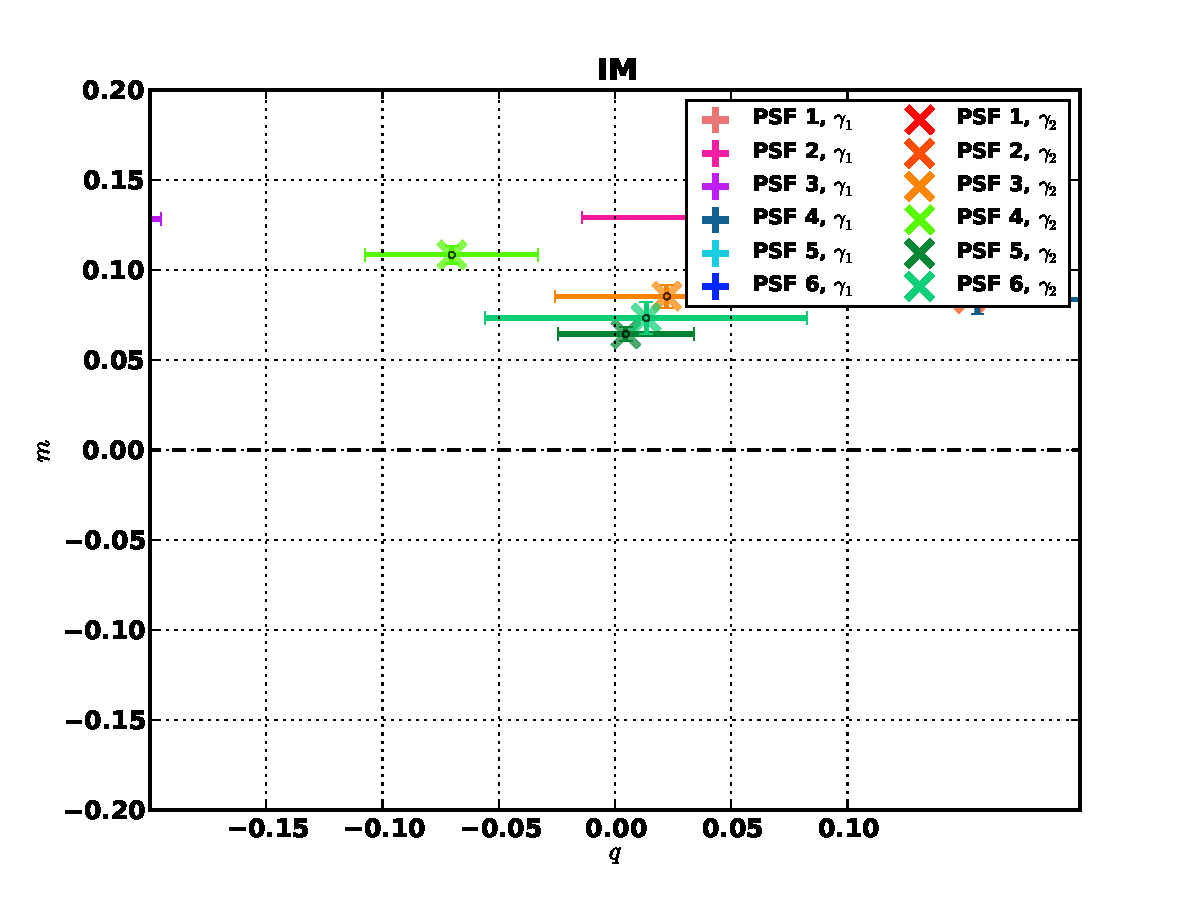
\includegraphics[width=0.45\textwidth]{fig/QMC_main_IM_f.pdf} 
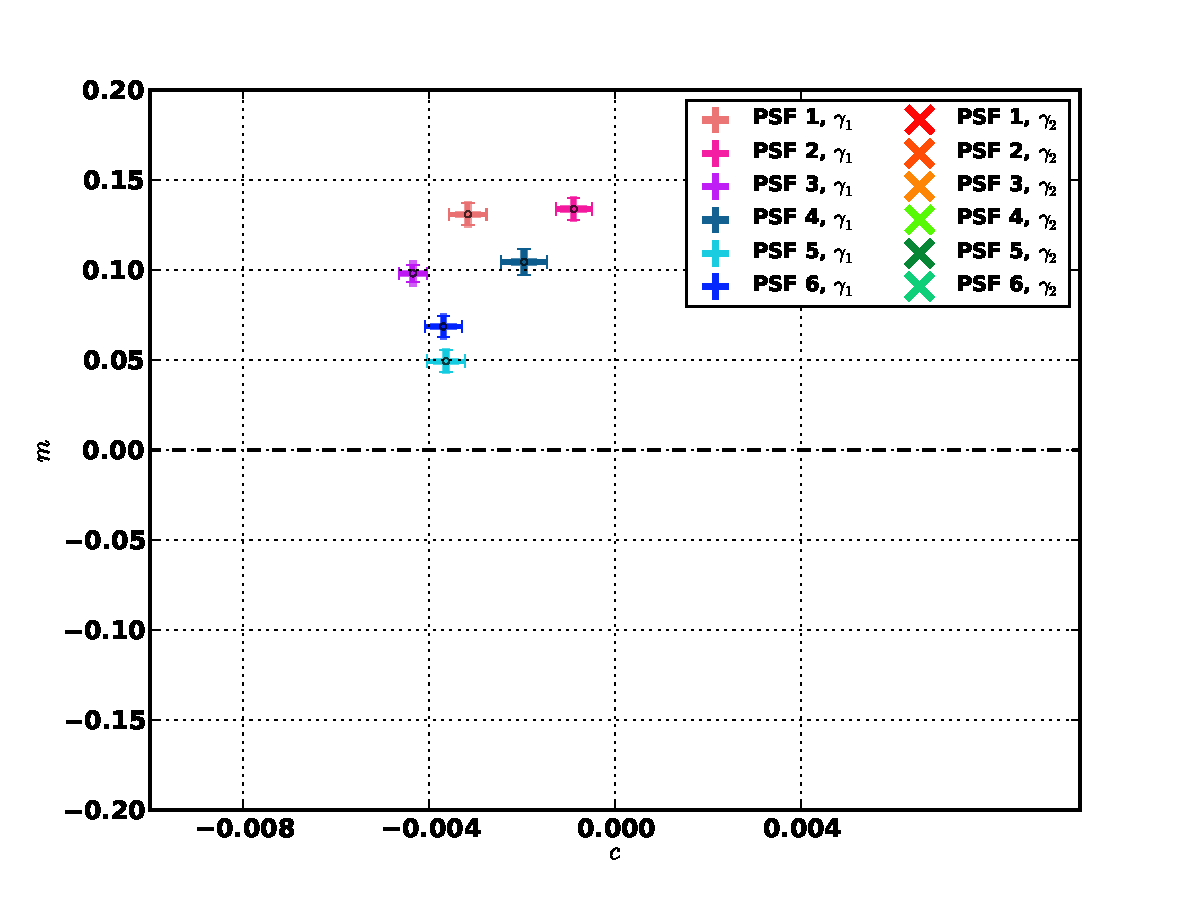
\includegraphics[width=0.45\textwidth]{fig/MC_main_IM_f.pdf} 
\caption{Average Q and M results for all pipelines for objects 
SNR $>$ 20 on the left and M and C results for all pipelines for objects 
SNR $>$ 20 on the right seperate by $\gamma_{1} $ and $\gamma_{2} $ as
well as PSF.}
\label{fig:IMCAT_qmc}
\end{figure*}

\begin{figure*}
\centering
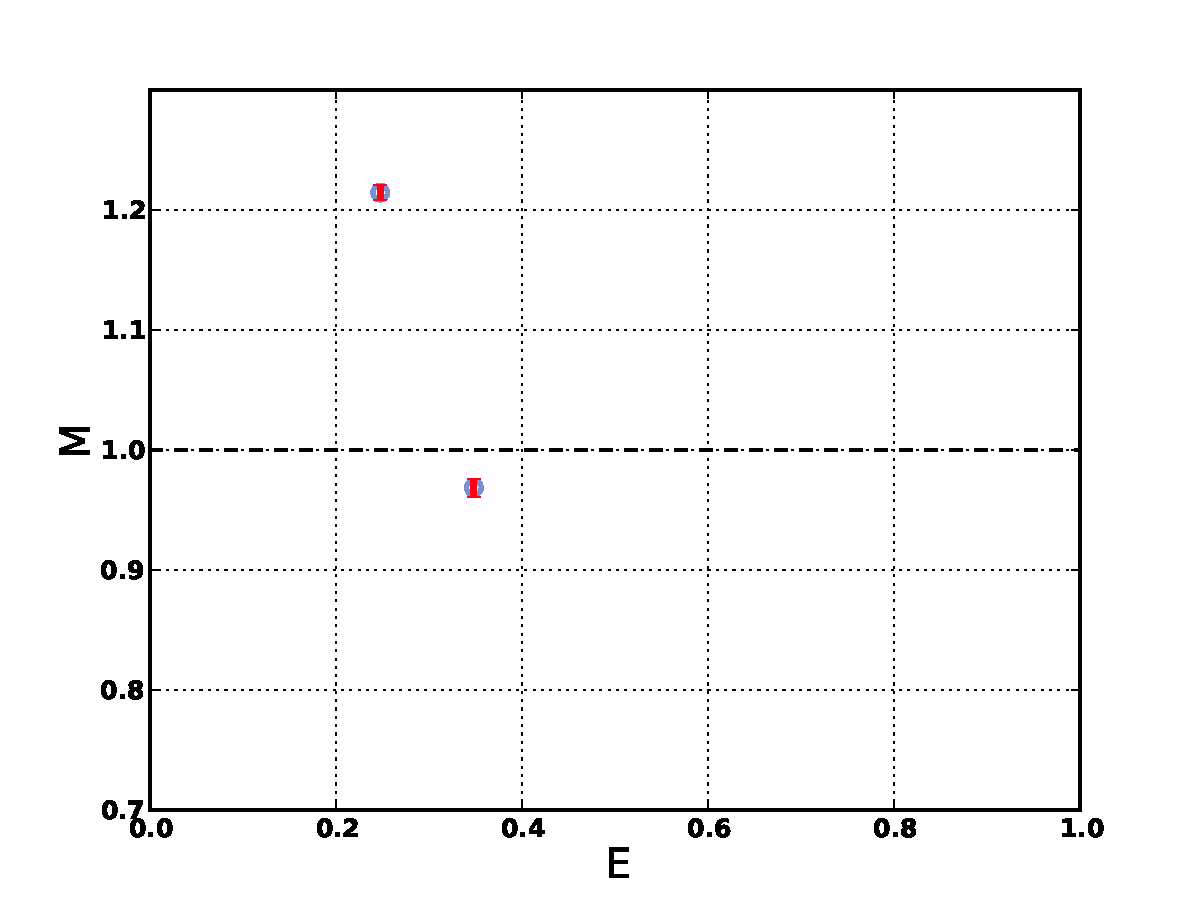
\includegraphics[width=0.45\textwidth]{fig/MvaleIM.pdf} 
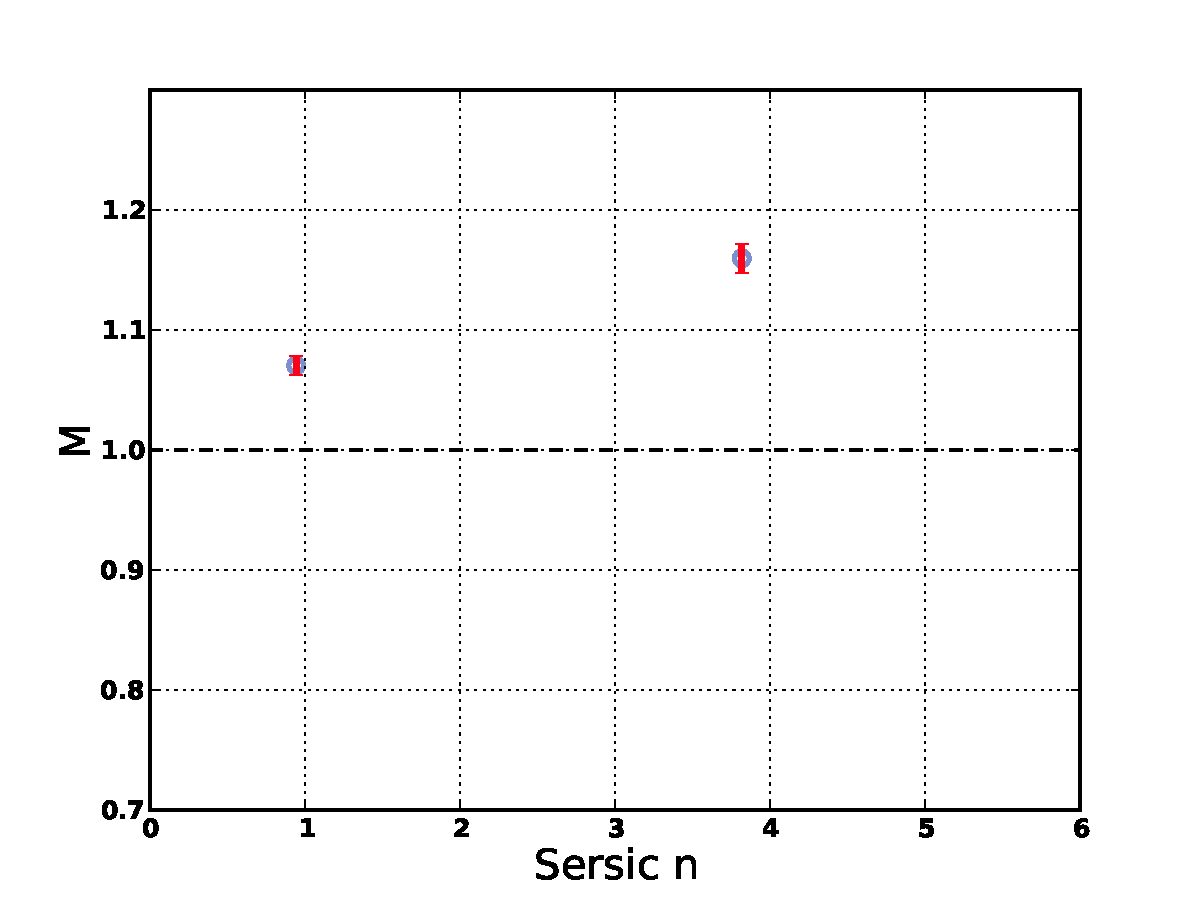
\includegraphics[width=0.45\textwidth]{fig/Mval_typeIM.pdf} 
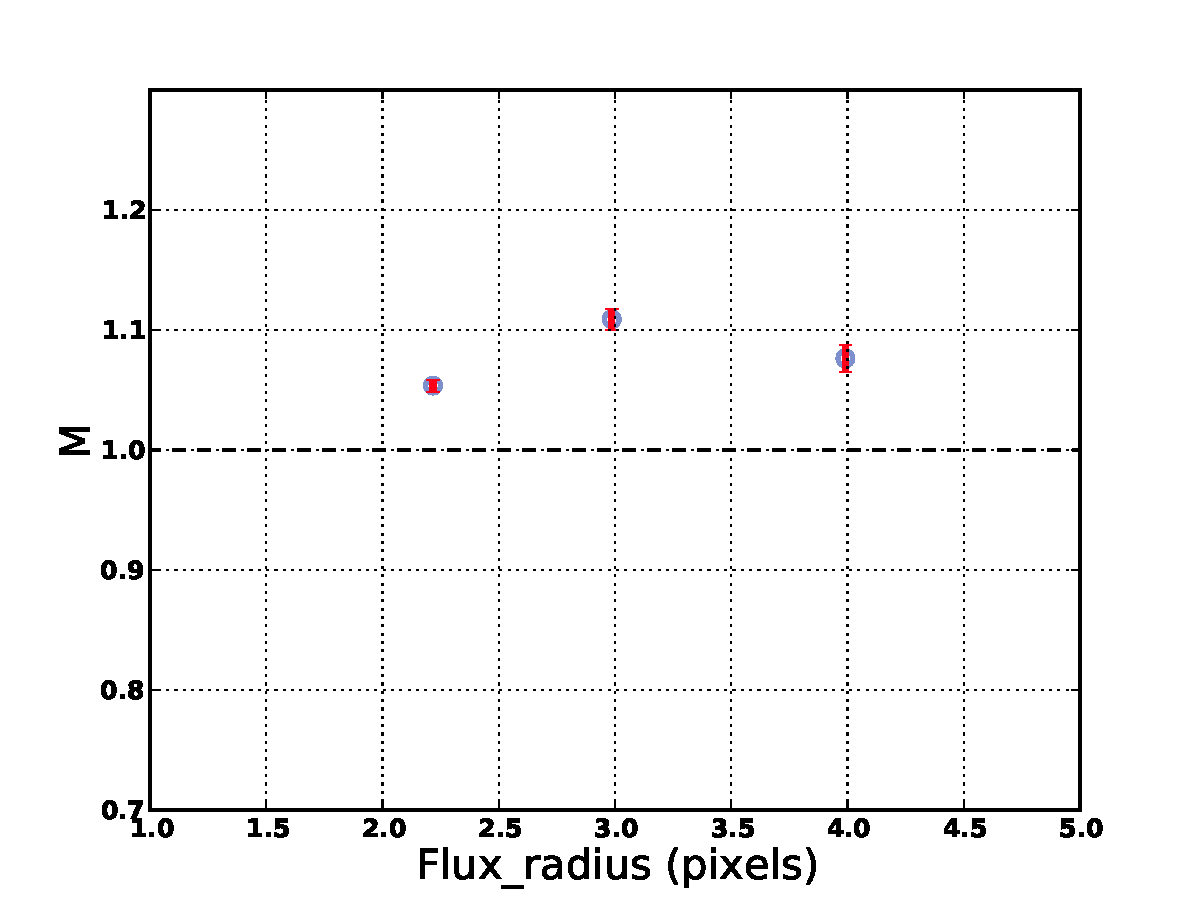
\includegraphics[width=0.45\textwidth]{fig/Mval_sizeIM.pdf} 
\caption{The M and C values for ...}
\label{fig:DEIMOS_m}
\end{figure*}

\newpage 
\subsection{ksbm}
The ksbm pipeline version used here is the same as the version
used to analyze the image sinulations in the GREAT10 challenge. This
KSB+ implementation uses elements of the 
DEMIOS lensing pipeline to determine the galaxy centroid and the
optimal size of the weighting function. There are no correction
factors applied, but objects with $\gamma > 1.0 $ are eliminated from
the final catalog. \\

\begin{figure*}
\centering
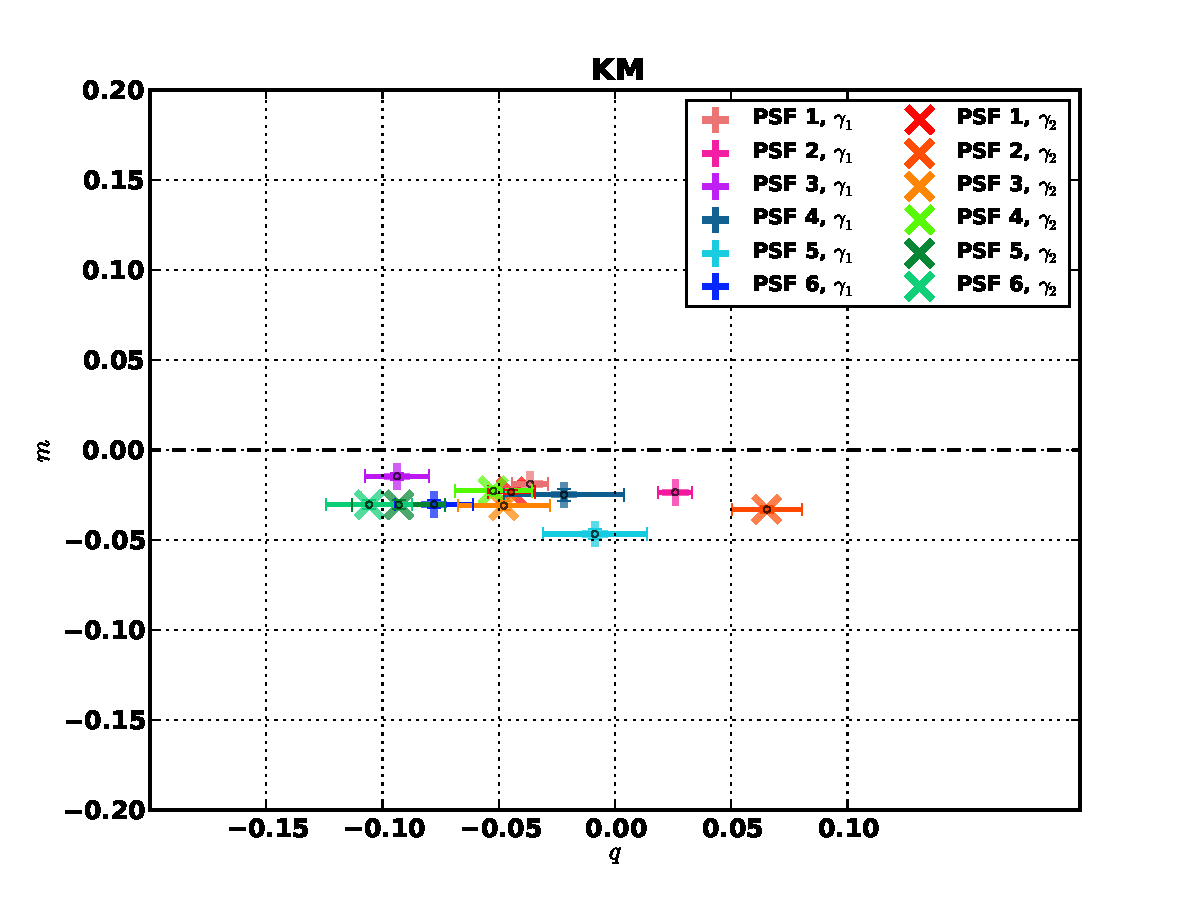
\includegraphics[width=0.45\textwidth]{fig/QMC_main_KM_f.pdf} 
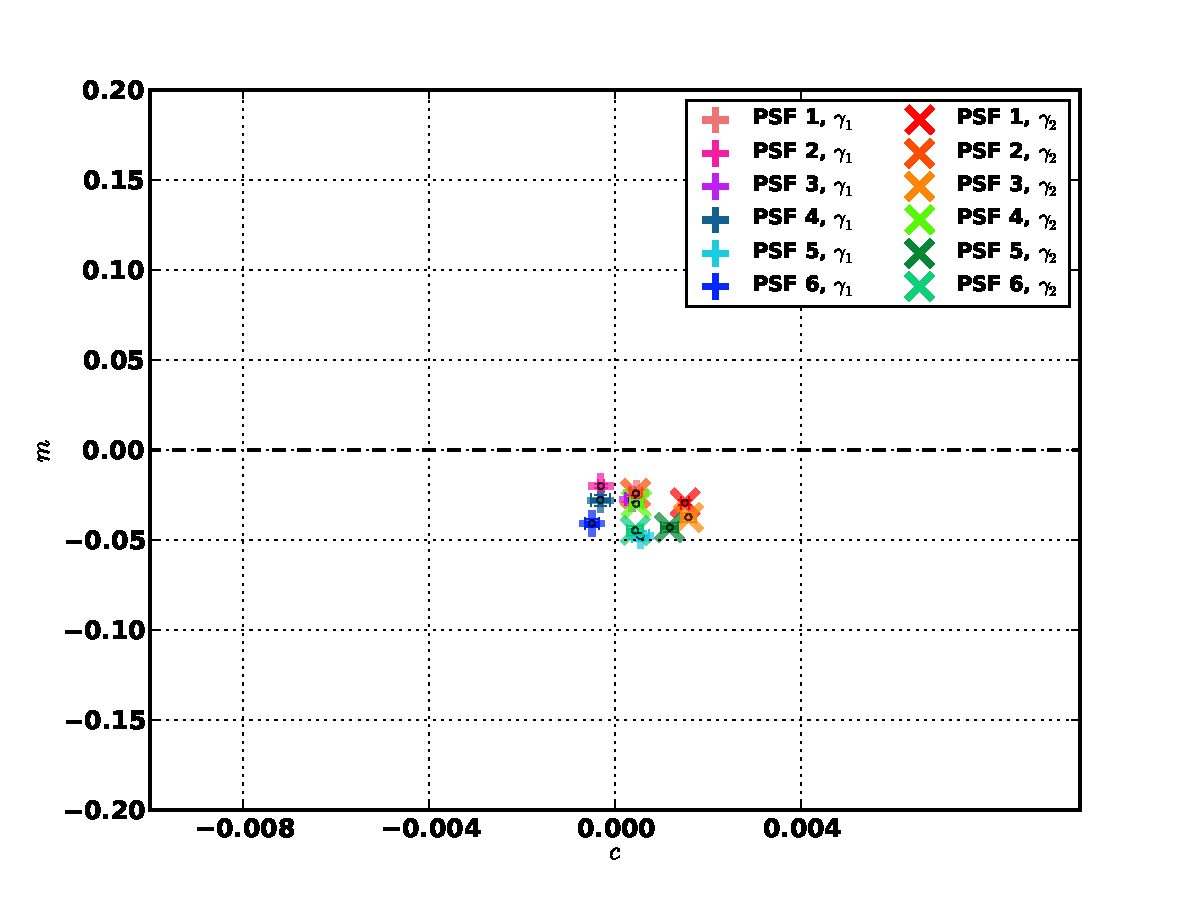
\includegraphics[width=0.45\textwidth]{fig/MC_main_KM_f.pdf} 
\caption{Average Q and M results for all pipelines for objects 
SNR $>$ 20 on the left and M and C results for all pipelines for objects 
SNR $>$ 20 on the right seperate by $\gamma_{1} $ and $\gamma_{2} $ as
well as PSF.}
\label{fig:ksbm_qmc}
\end{figure*}

\begin{figure*}
\centering
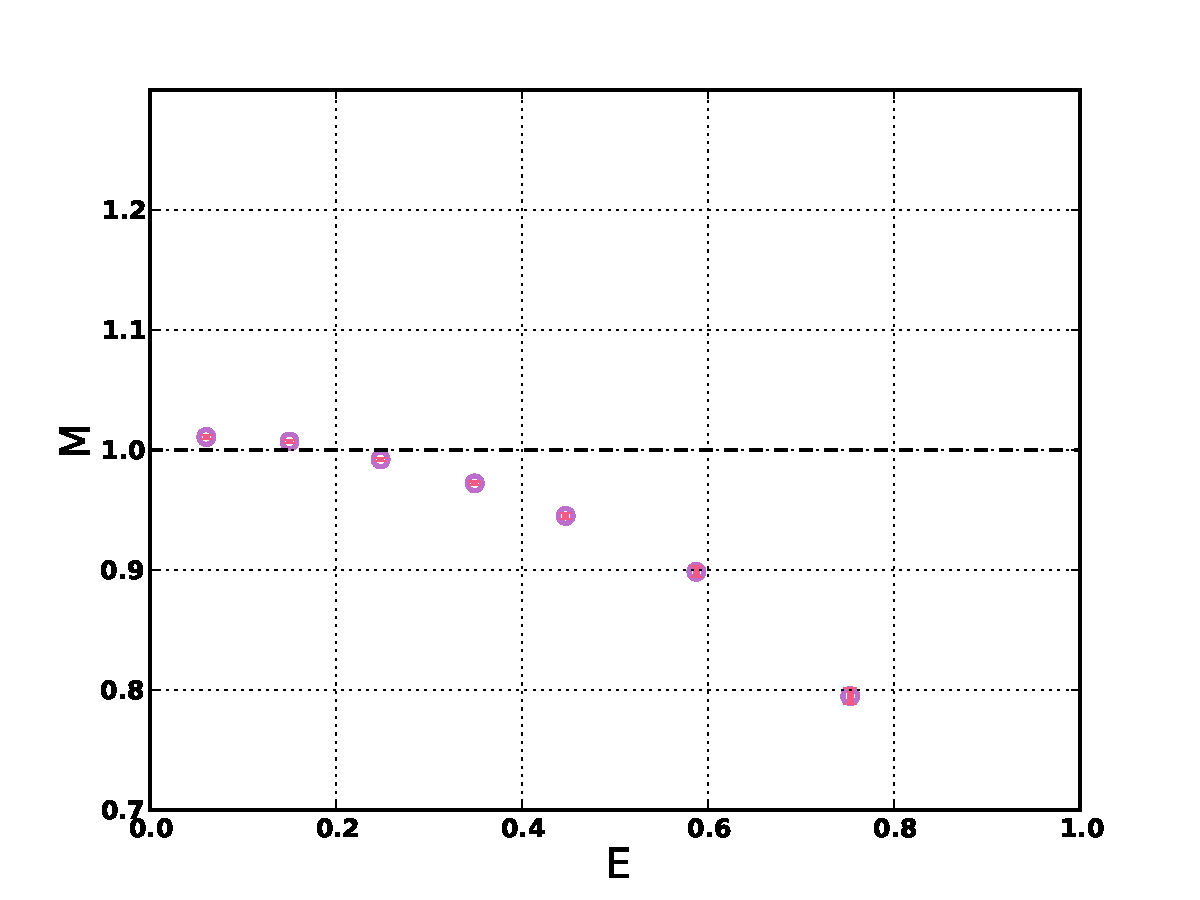
\includegraphics[width=0.45\textwidth]{fig/MvaleKM.pdf} 
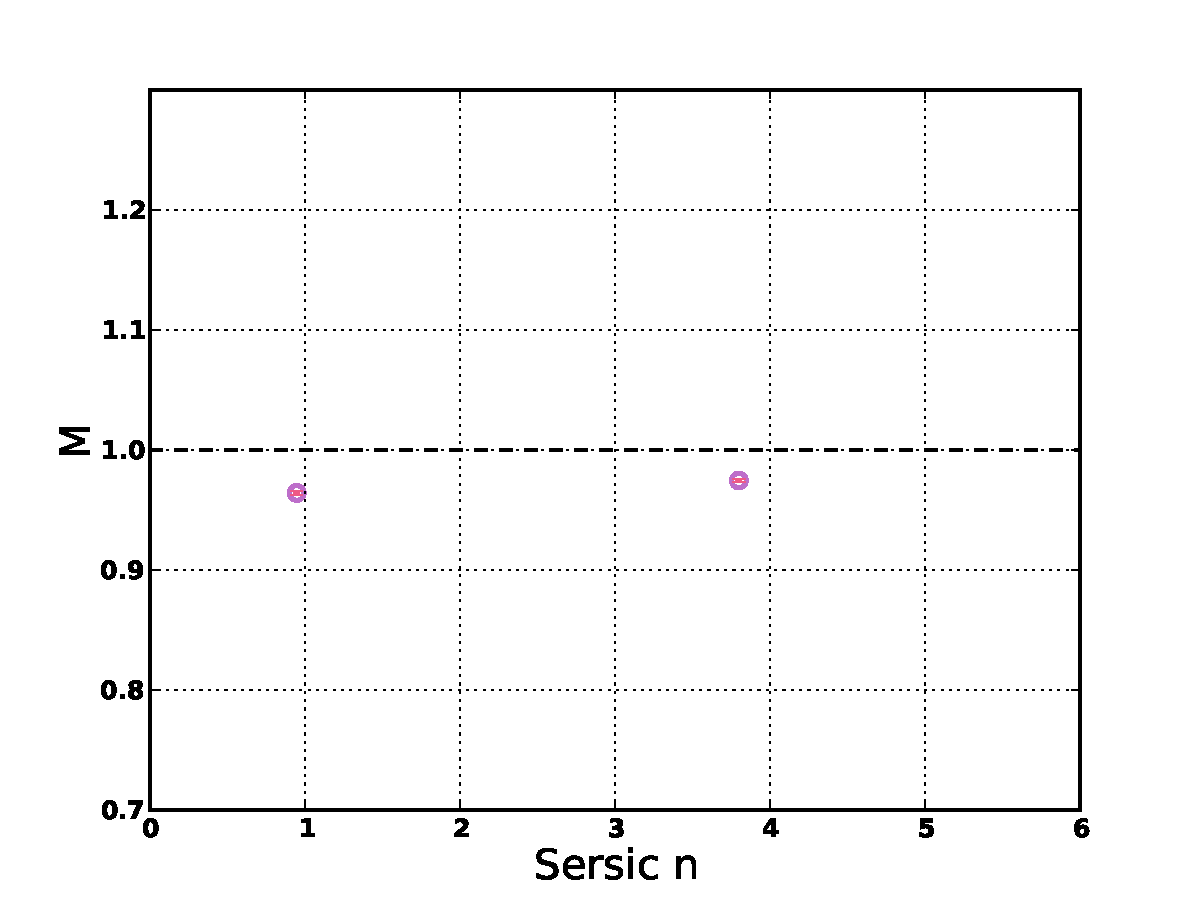
\includegraphics[width=0.45\textwidth]{fig/Mval_typeKM.pdf} 
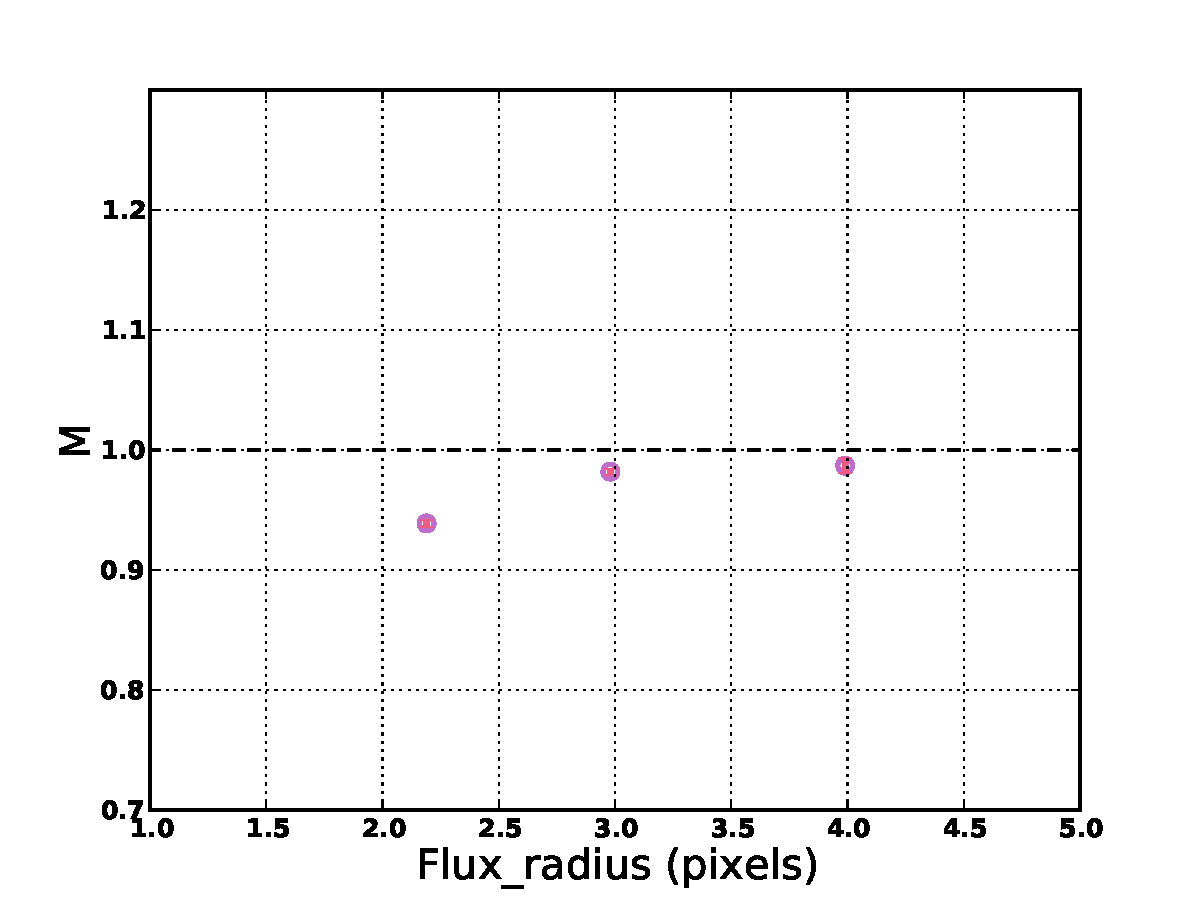
\includegraphics[width=0.45\textwidth]{fig/Mval_sizeKM.pdf} 
\caption{The M and C values for ...}
\label{fig:DEIMOS_m}
\end{figure*}

\newpage 
\subsection{PKSB}
PKSB is a lensing pipeline that uses the PSFEx \cite{PSFex}
to create a model of the PSF and an implementation of KSB+ method 
for shape measurement. A modified version of this lensing pipeline
that incorperates correction of shape measurement bias, based on the
CSTEP simulations, has been used to measure the mass of galaxy
clusters in \cite{Gruen_s} and \cite{Gruen2}. \\
 
\begin{figure*}
\centering
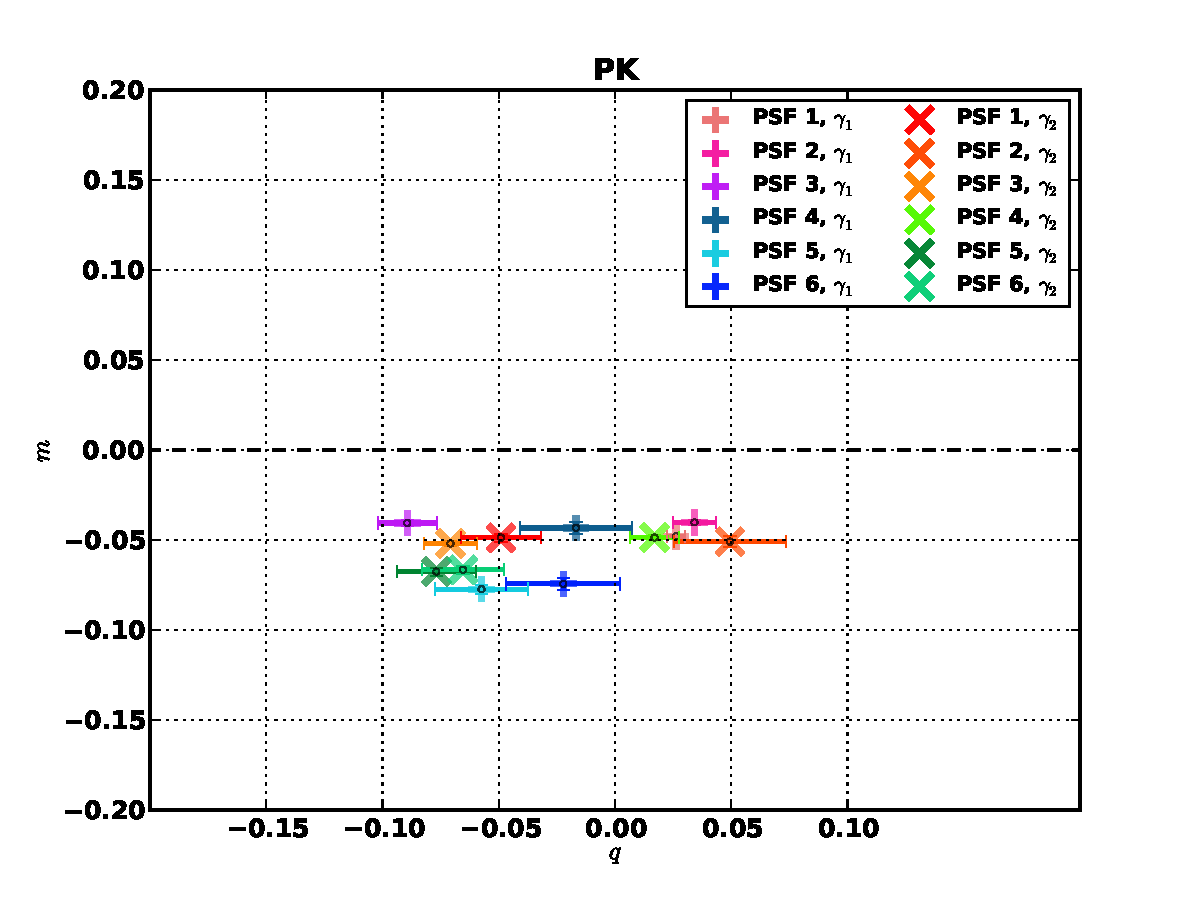
\includegraphics[width=0.45\textwidth]{fig/QMC_main_PK_f.pdf} 
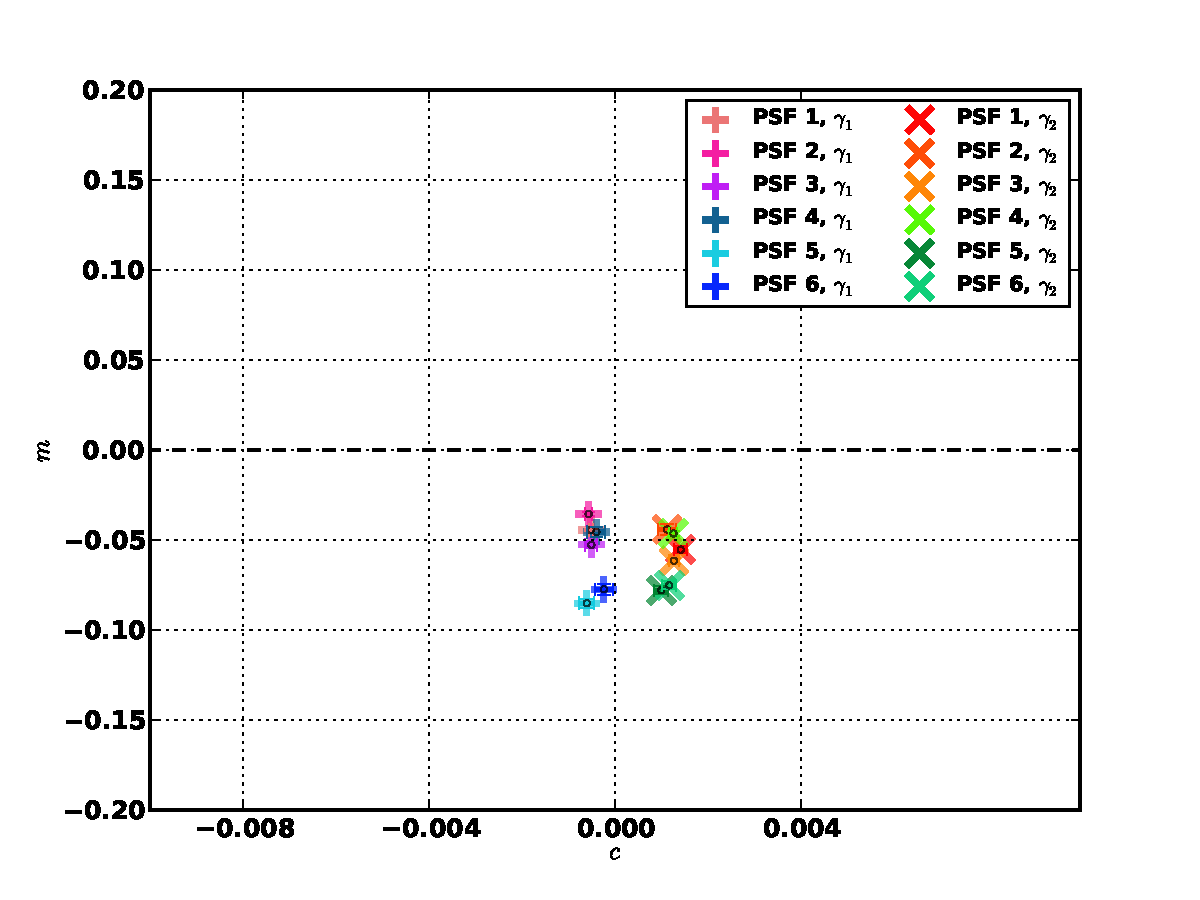
\includegraphics[width=0.45\textwidth]{fig/MC_main_PK_f.pdf} 
\caption{Average Q and M results for all pipelines for objects 
SNR $>$ 20 on the left and M and C results for all pipelines for objects 
SNR $>$ 20 on the right seperate by $\gamma_{1} $ and $\gamma_{2} $ as
well as PSF.}
\label{fig:PKSB_qmc}
\end{figure*}

\begin{figure*}
\centering
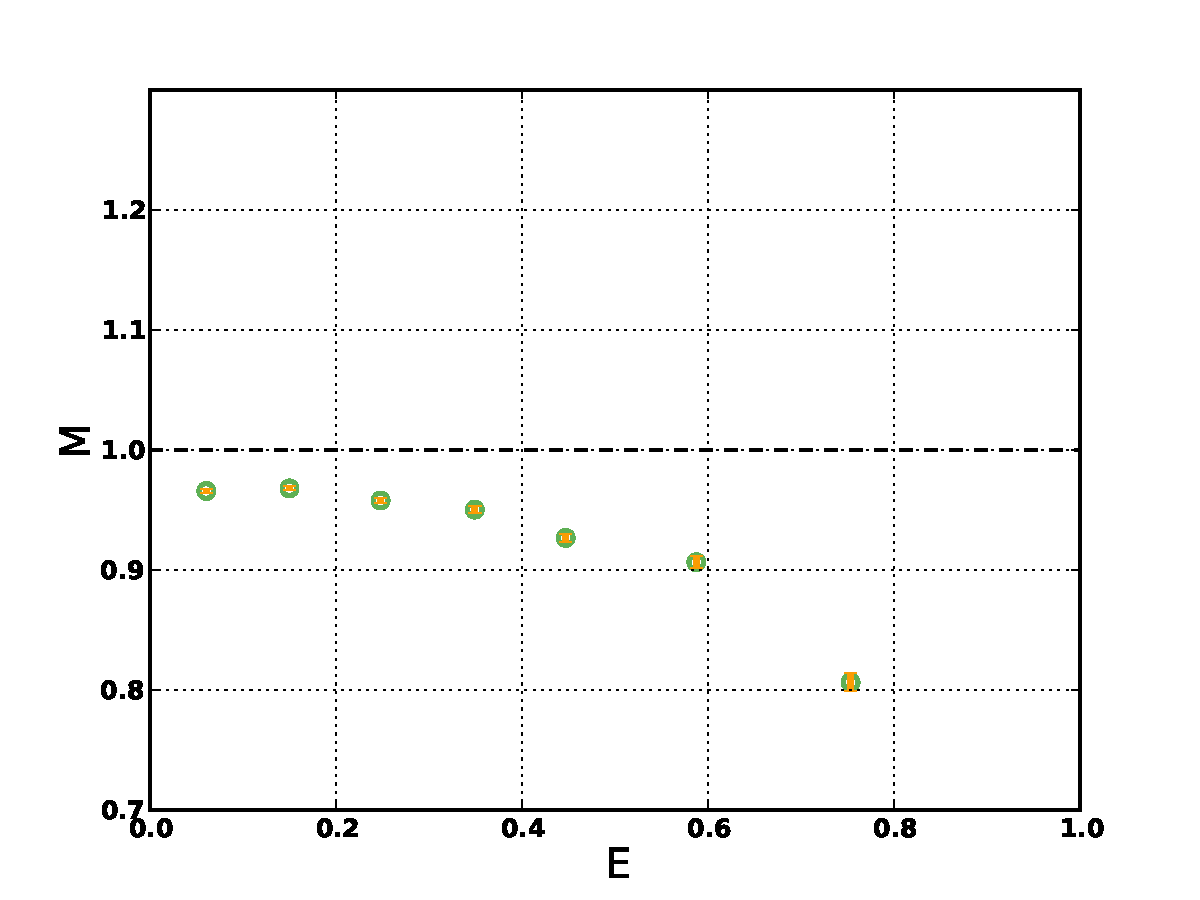
\includegraphics[width=0.45\textwidth]{fig/MvalePK.pdf} 
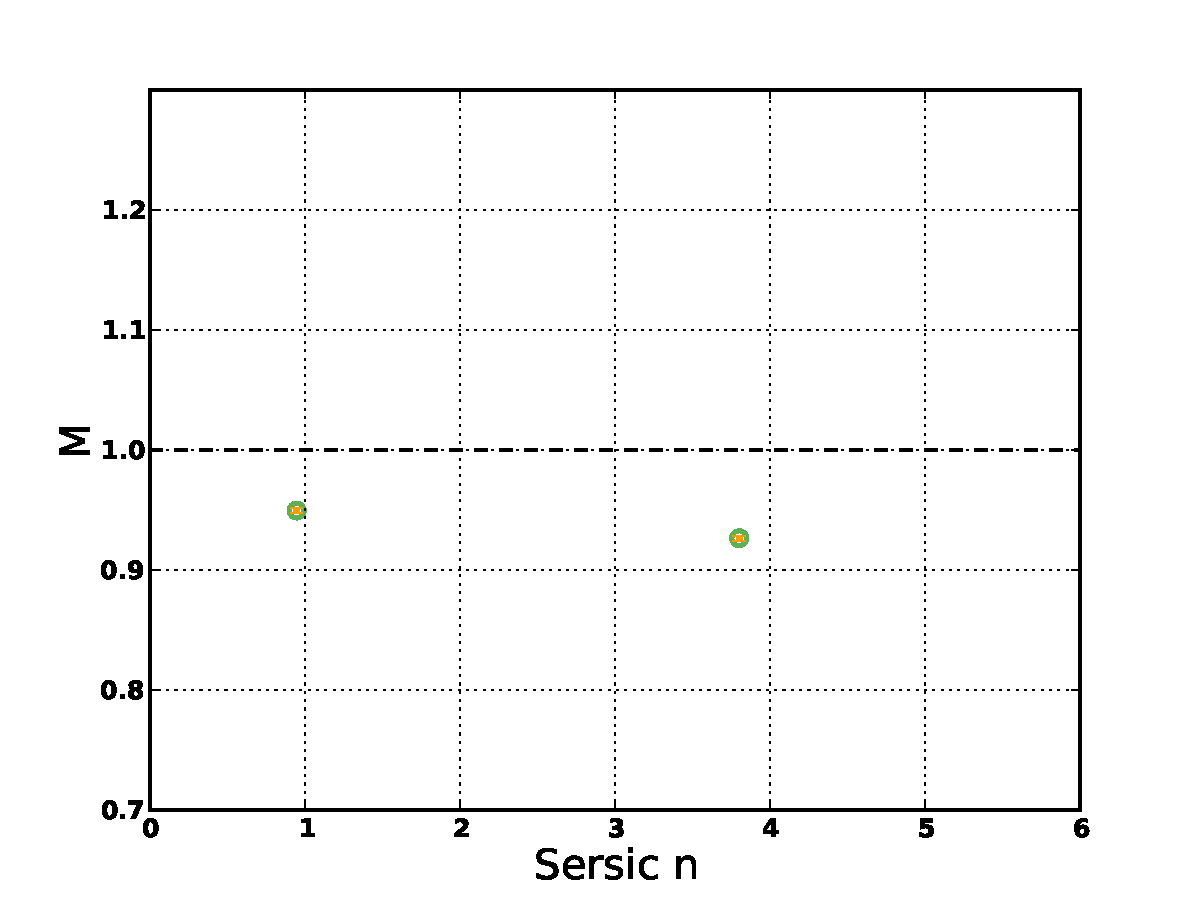
\includegraphics[width=0.45\textwidth]{fig/Mval_typePK.pdf} 
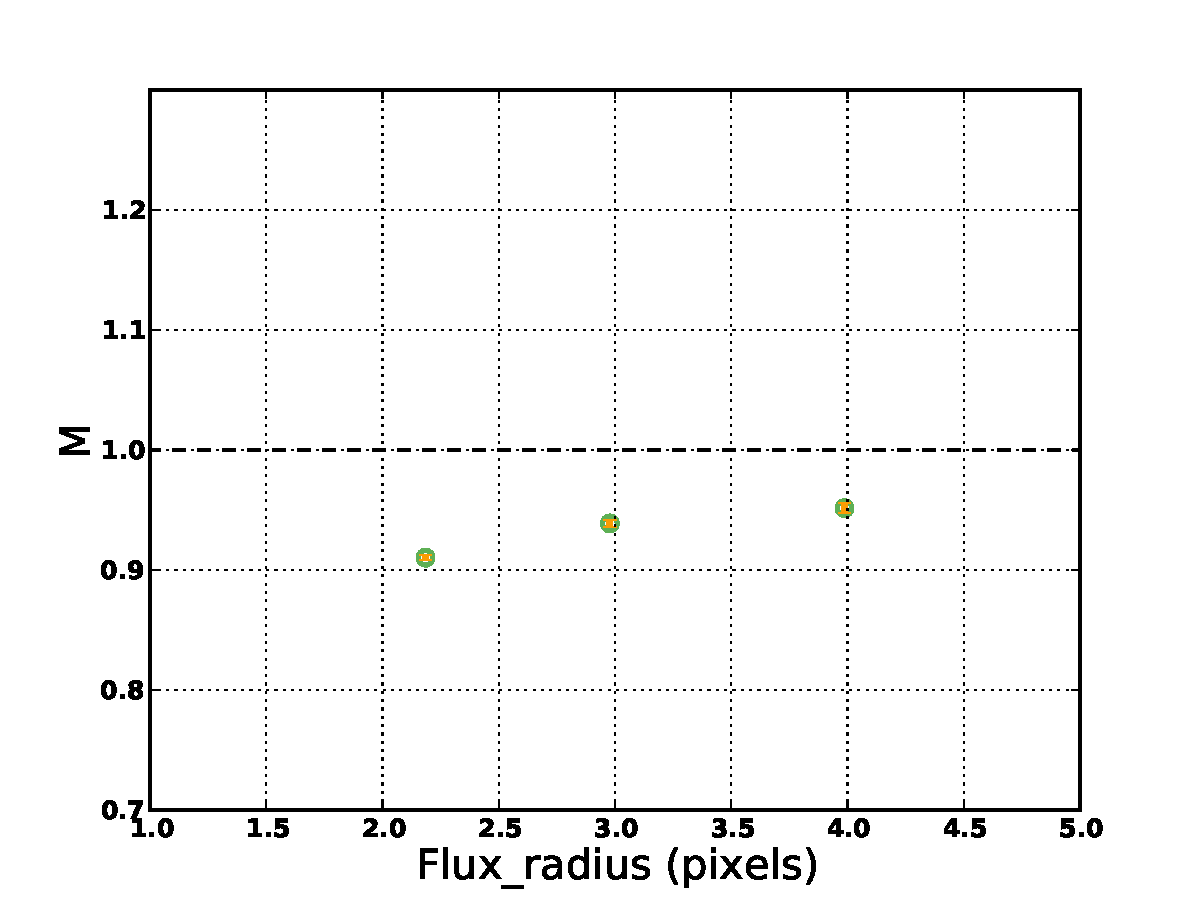
\includegraphics[width=0.45\textwidth]{fig/Mval_sizePK.pdf} 
\caption{The M and C values for ...}
\label{fig:DEIMOS_m}
\end{figure*}

\newpage 
\subsection{Gaussian Mixtures}
\begin{figure*}
\centering
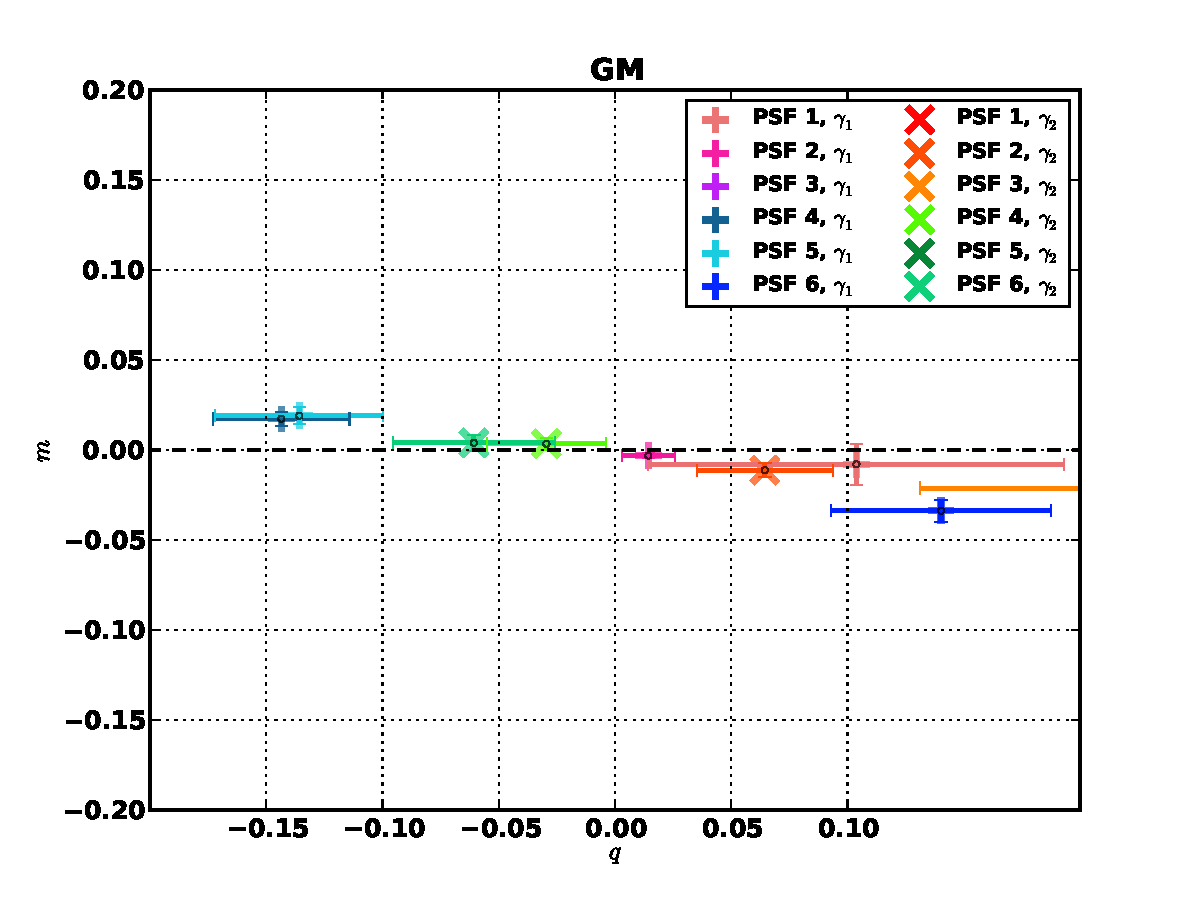
\includegraphics[width=0.45\textwidth]{fig/QMC_main_GM_f.pdf} 
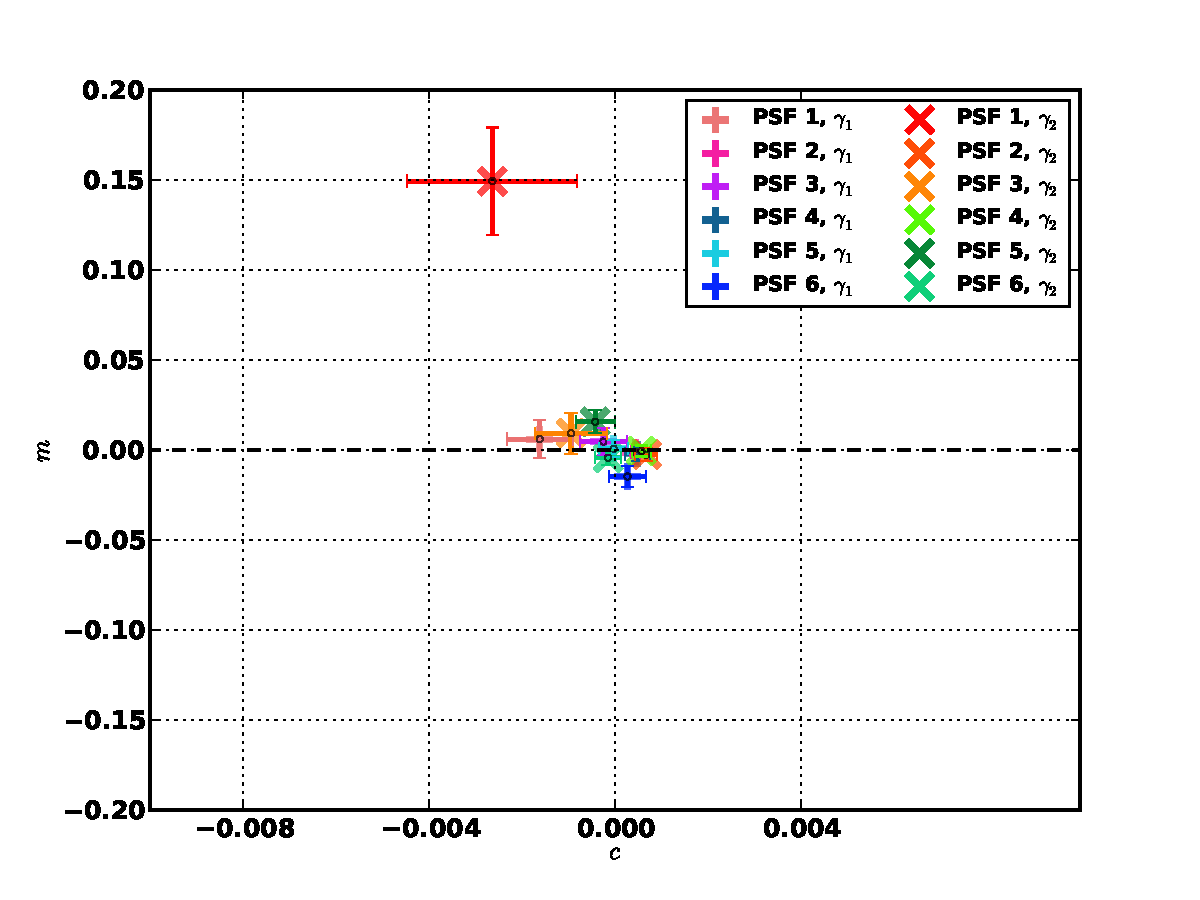
\includegraphics[width=0.45\textwidth]{fig/MC_main_GM_f.pdf} 
\caption{Average Q and M results for all pipelines for objects 
SNR $>$ 20 on the left and M and C results for all pipelines for objects 
SNR $>$ 20 on the right seperate by $\gamma_{1} $ and $\gamma_{2} $ as
well as PSF.}
\label{fig:Gmix_qmc}
\end{figure*}

\begin{figure*}
\centering
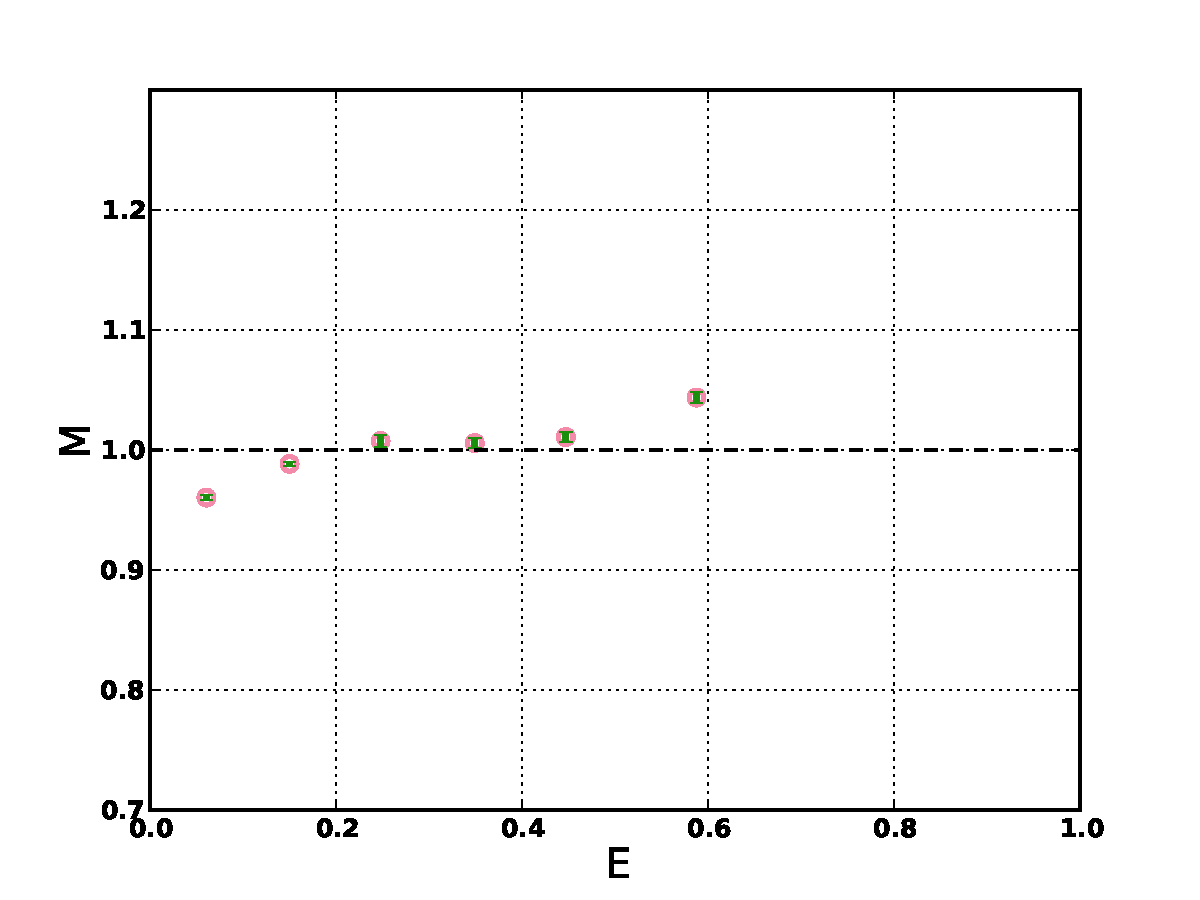
\includegraphics[width=0.45\textwidth]{fig/MvaleGM.pdf} 
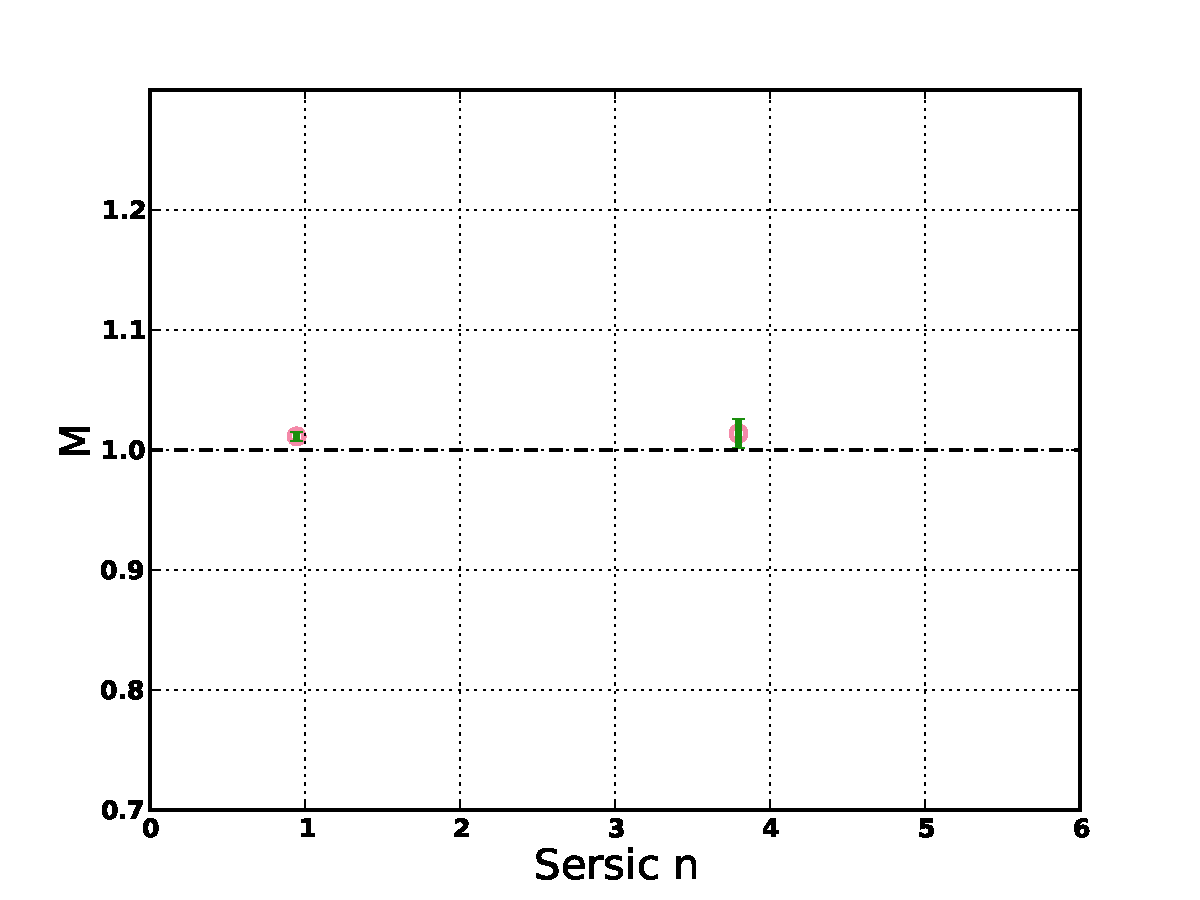
\includegraphics[width=0.45\textwidth]{fig/Mval_typeGM.pdf} 
%\includegraphics[width=0.45\textwidth]{fig/Mval_sizeGM.pdf} 
\caption{The M and C values for ...}
\label{fig:DEIMOS_m}
\end{figure*}

\newpage 
\subsection{im3shape}
im3shape is a modular shape measurement code that performs a maximum likelihood (ML) fit of a de Vaucouleurs bulge plus Exponential disc galaxy model to noisy images, incorporating an applied PSF (see Zuntz et al 2013/in prep.).  The software is written primarily in C with supporting Python infrastructure, and is publicly available.  For the ClusterSTEP data the PSF is modelled as an elliptical Moffat profile (1969), assumed to be constant across each chip.  Moffat profiles were fit (using the Levenberg-Marquardt algorithm) to stellar images in the ClusterSTEP data, and the chipwise model estimated from these individual fits using an inverse variance weighted average of the resulting best-fitting parameters. For the subset of fields in which the PSF was known to be Gaussian, a $\beta$ slope parameter of 1000 was fixed in the profile fitting process (the Moffat approaches the Gaussian profile for large $\beta$).

For galaxy shape measurement using parametric profiles, ML estimators are known to be biased due to the presence of noise (e.g., Refregier et al 2012; Kacprzak et al 2012).  For the tests in this paper a suite of noise bias-calibrating simulations were not conducted, due to resource constraints and the challenge of producing a representative calibration suite for data with realistic distributions of size and signal-to-noise such as ClusterSTEP:  the noise calibration schemes presented by Kacprzak et al (2012) and Zuntz et al (2013) were for far simpler distributions of galaxy properties.  Understanding how to build such suites is an active field of research, and of great relevance to the many methods with known noise bias issues.

The performance of im3shape shear estimates is therefore expected to degrade somewhat as signal-to-noise decreases.  Objects with an im3shape-determined signal-to-noise (in total flux) of lower than 10 were excluded in the final catalogue, along with catastrophic outliers in the value of the best likelihood, and objects for which any pixel value in a model-minus-data residual image was found to be greater than the peak pixel flux in the data.
\begin{figure*}
\centering
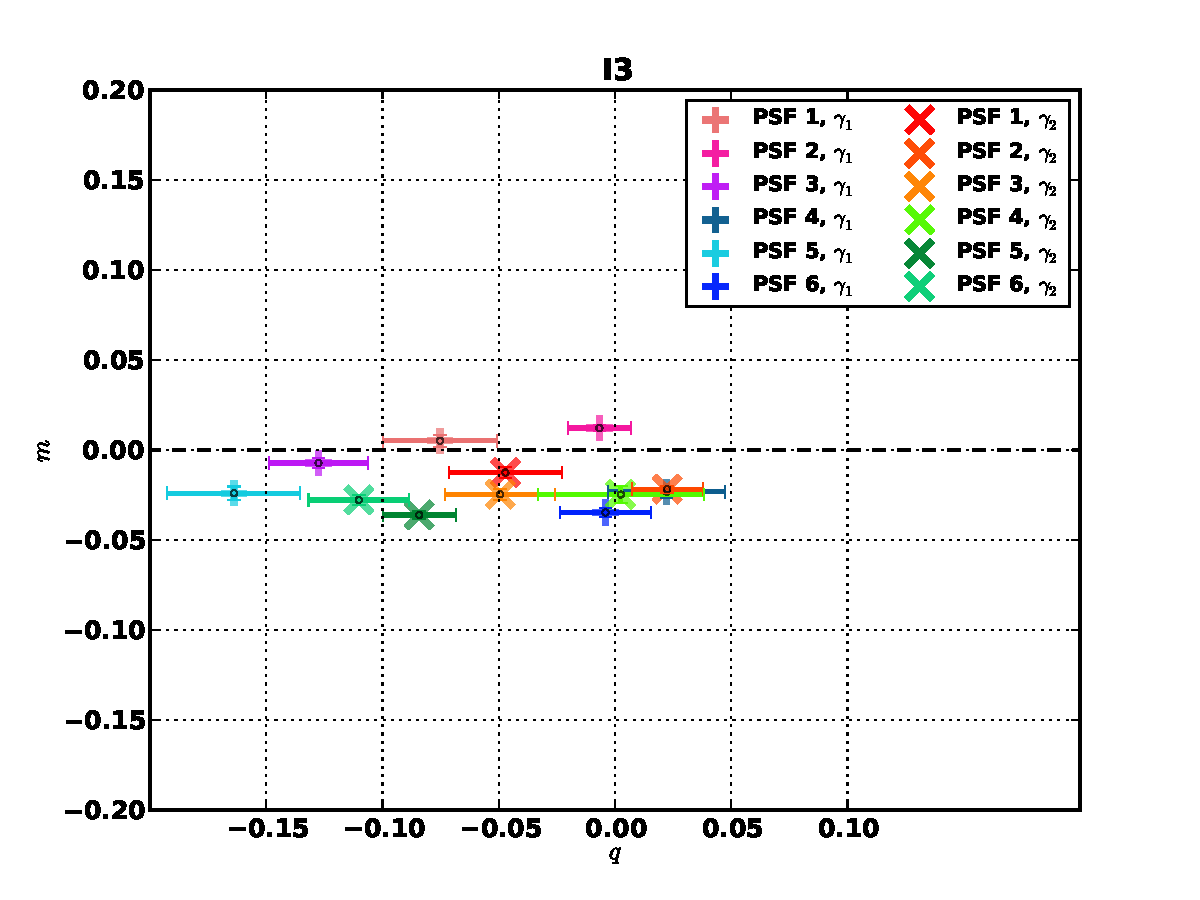
\includegraphics[width=0.45\textwidth]{fig/QMC_main_I3_f.pdf} 
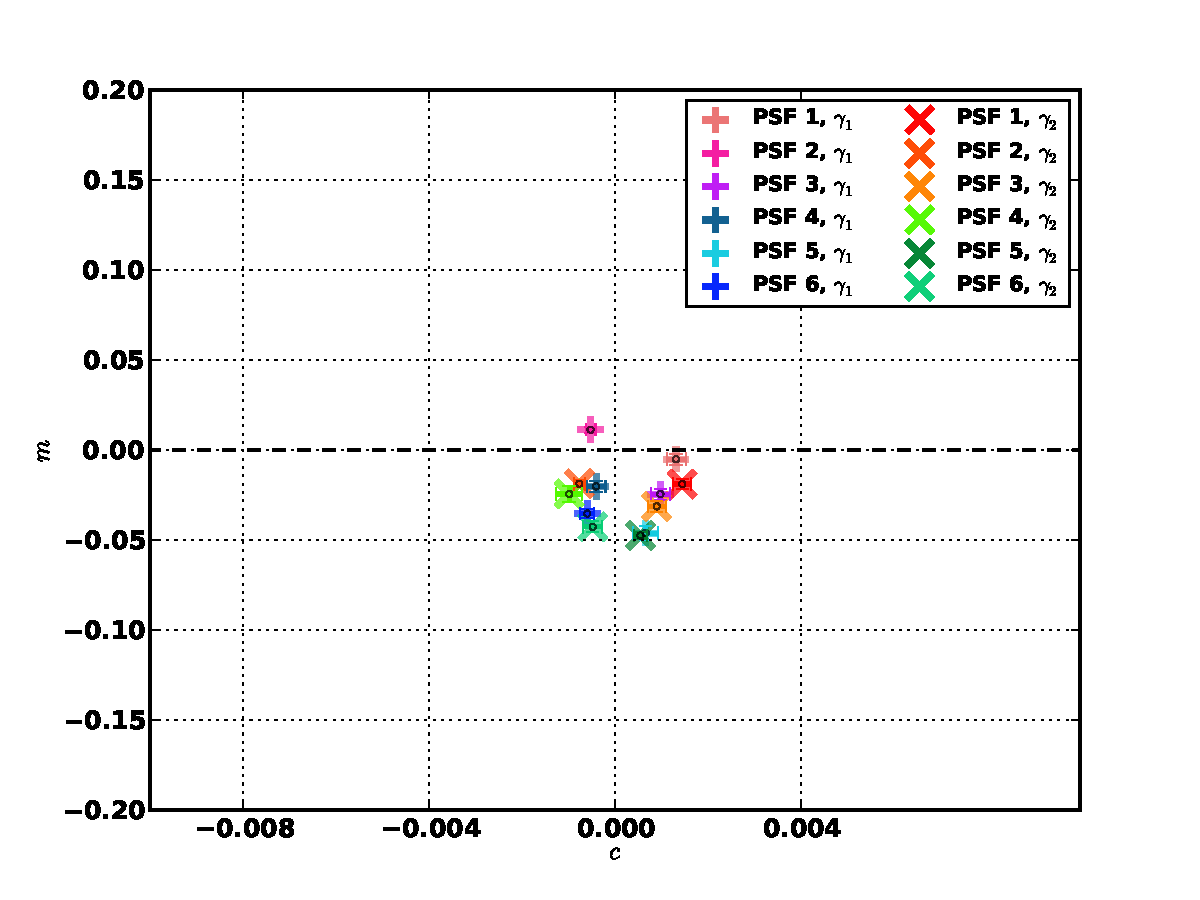
\includegraphics[width=0.45\textwidth]{fig/MC_main_I3_f.pdf} 
\caption{Average Q and M results for all pipelines for objects 
SNR $>$ 20 on the left and M and C results for all pipelines for objects 
SNR $>$ 20 on the right seperate by $\gamma_{1} $ and $\gamma_{2} $ as
well as PSF.}
\label{fig:im3shape_qmc}
\end{figure*}

\begin{figure*}
\centering
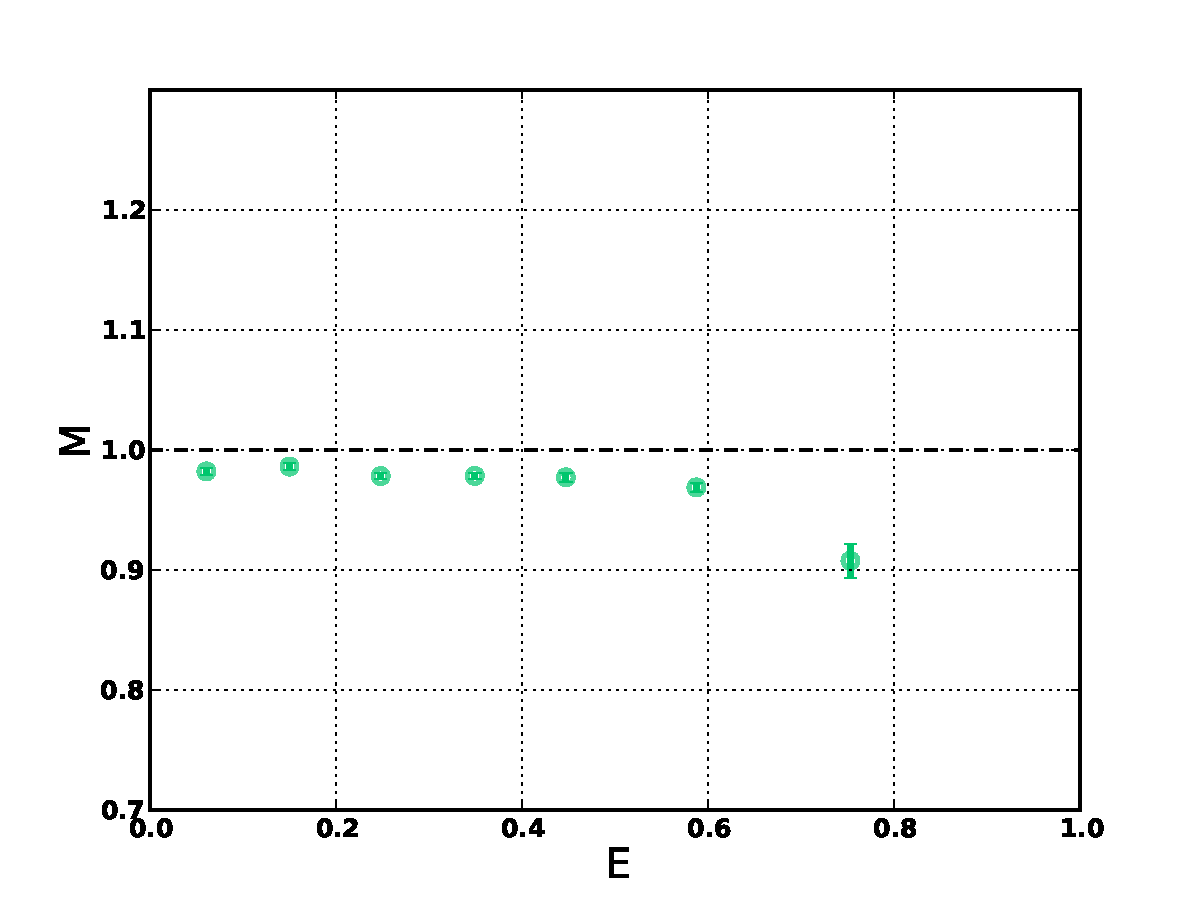
\includegraphics[width=0.45\textwidth]{fig/MvaleI3.pdf} 
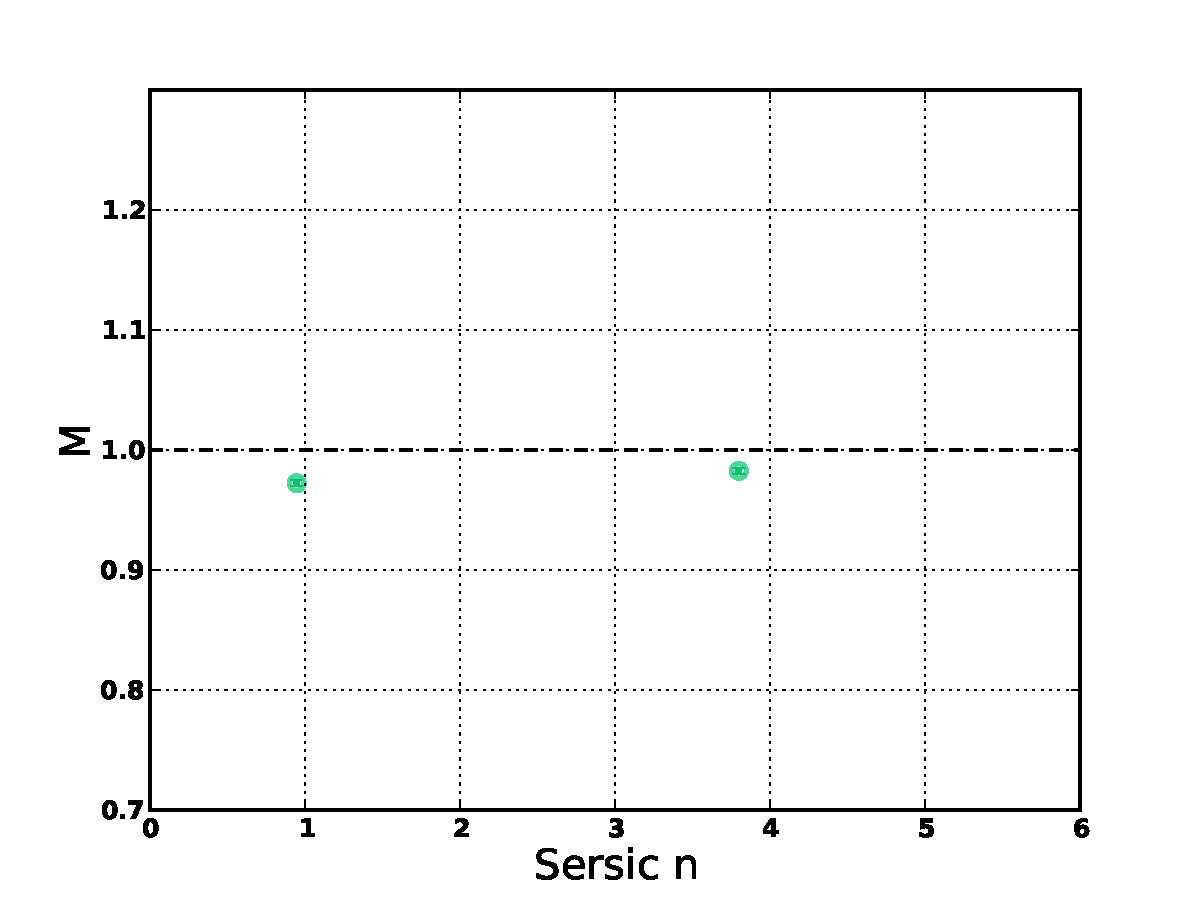
\includegraphics[width=0.45\textwidth]{fig/Mval_typeI3.pdf} 
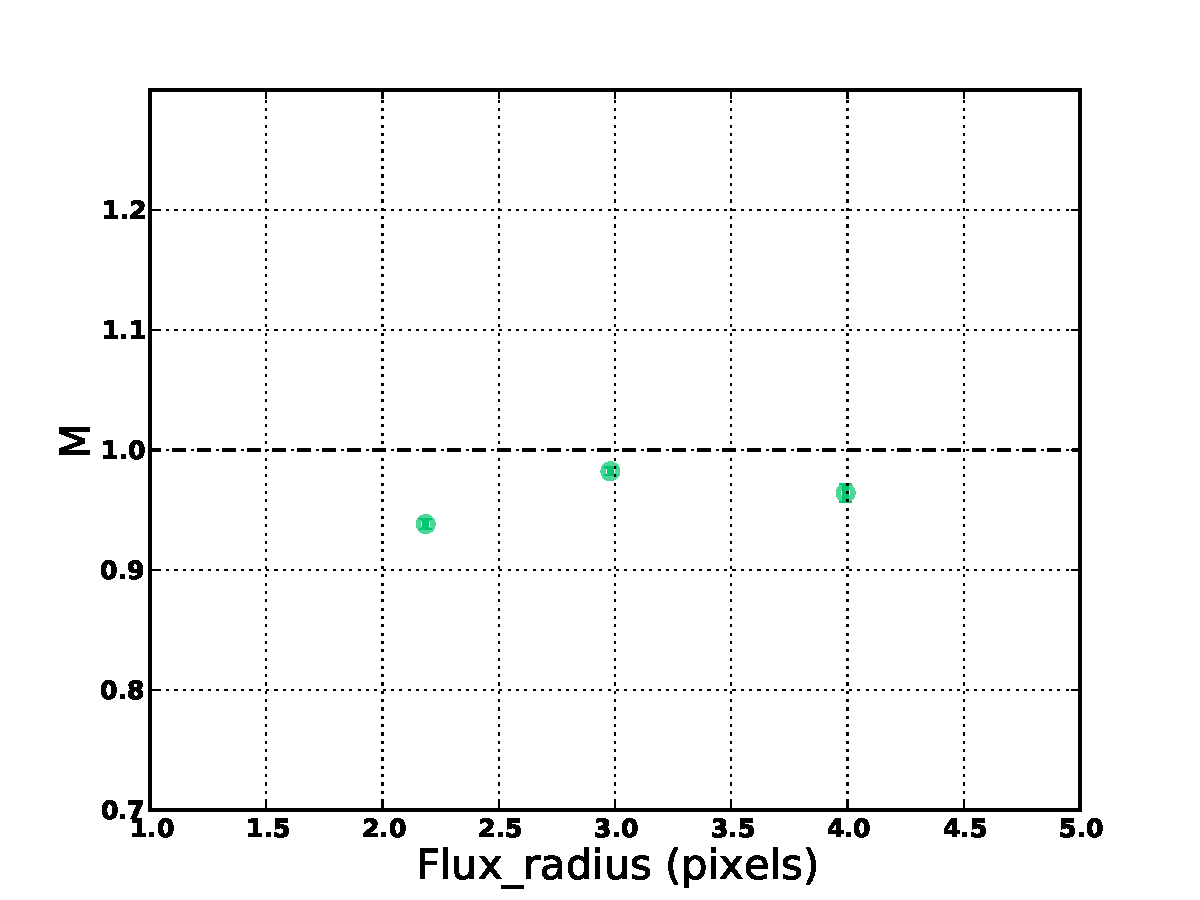
\includegraphics[width=0.45\textwidth]{fig/Mval_sizeI3.pdf} 
\caption{The M and C values for ...}
\label{fig:DEIMOS_m}
\end{figure*}

\newpage 
\subsection{BJ02}
\begin{figure*}
\centering
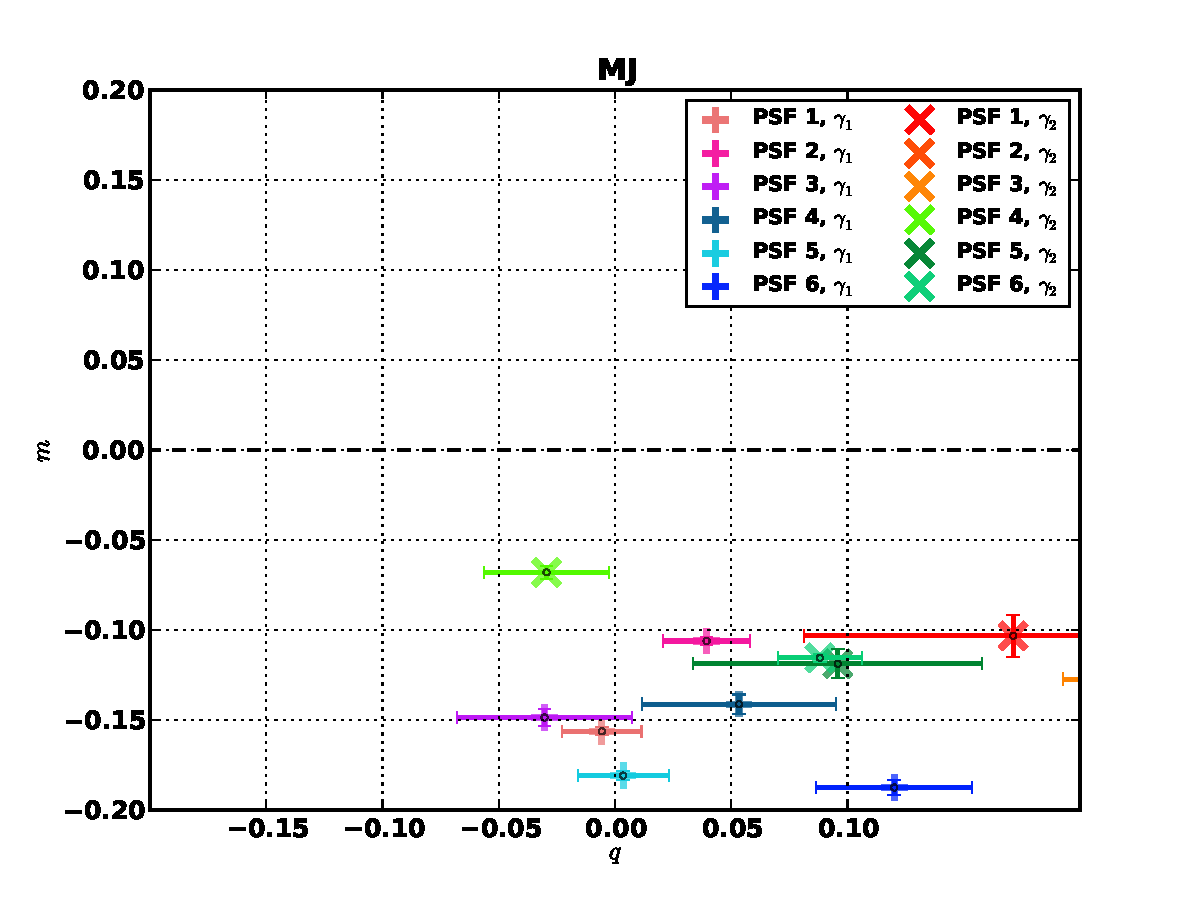
\includegraphics[width=0.45\textwidth]{fig/QMC_main_MJ_f.pdf} 
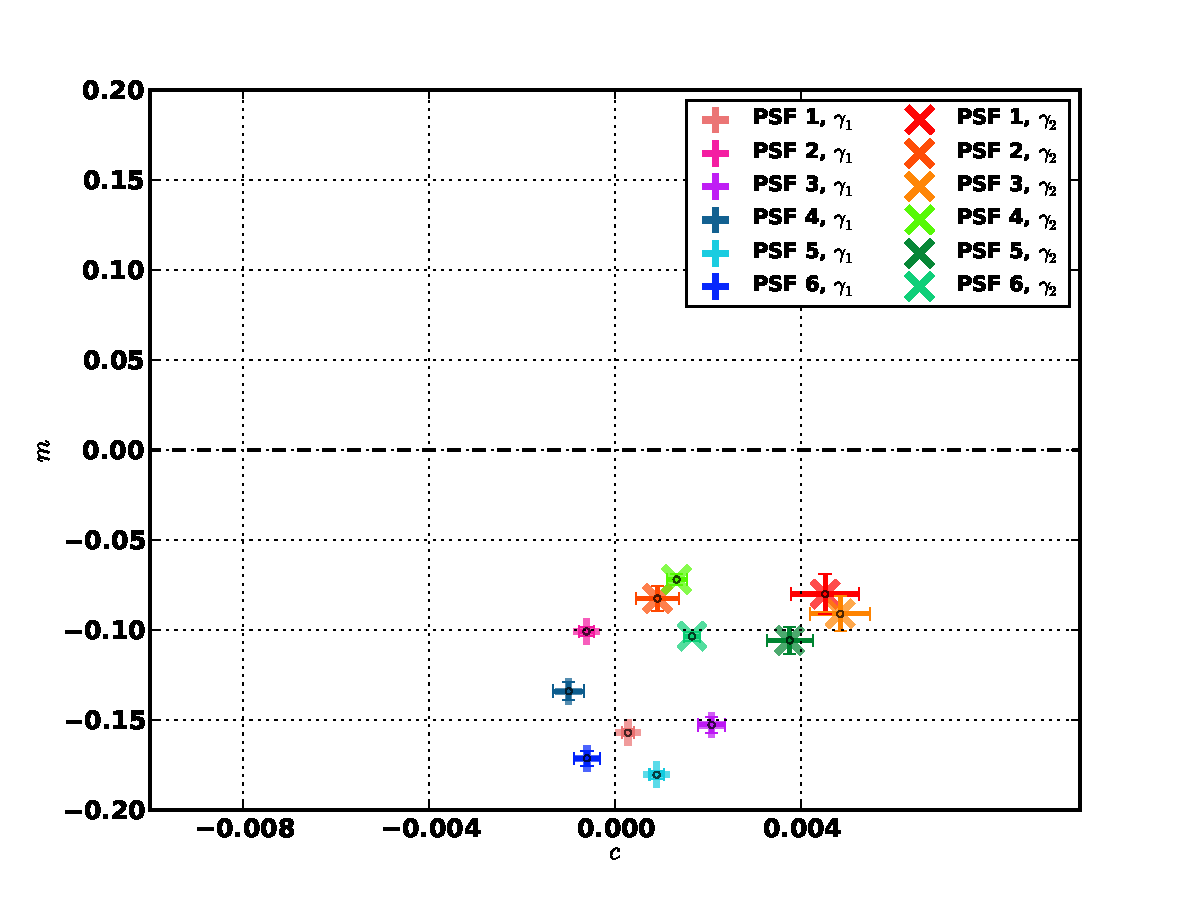
\includegraphics[width=0.45\textwidth]{fig/MC_main_MJ_f.pdf} 
\caption{Average Q and M results for all pipelines for objects 
SNR $>$ 20 on the left and M and C results for all pipelines for objects 
SNR $>$ 20 on the right seperate by $\gamma_{1} $ and $\gamma_{2} $ as
well as PSF.}
\label{fig:BJ_qmc}
\end{figure*}

\begin{figure*}
\centering
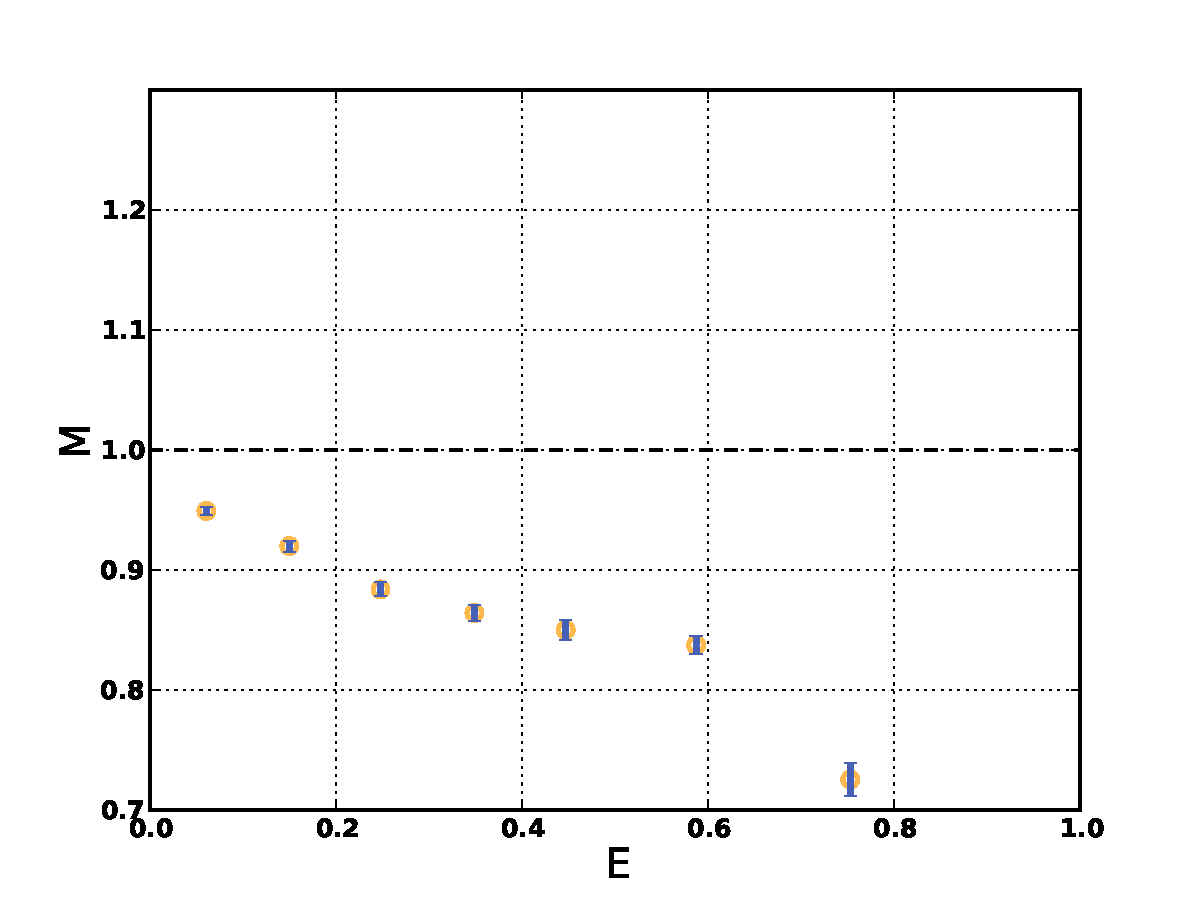
\includegraphics[width=0.45\textwidth]{fig/MvaleMJ.pdf} 
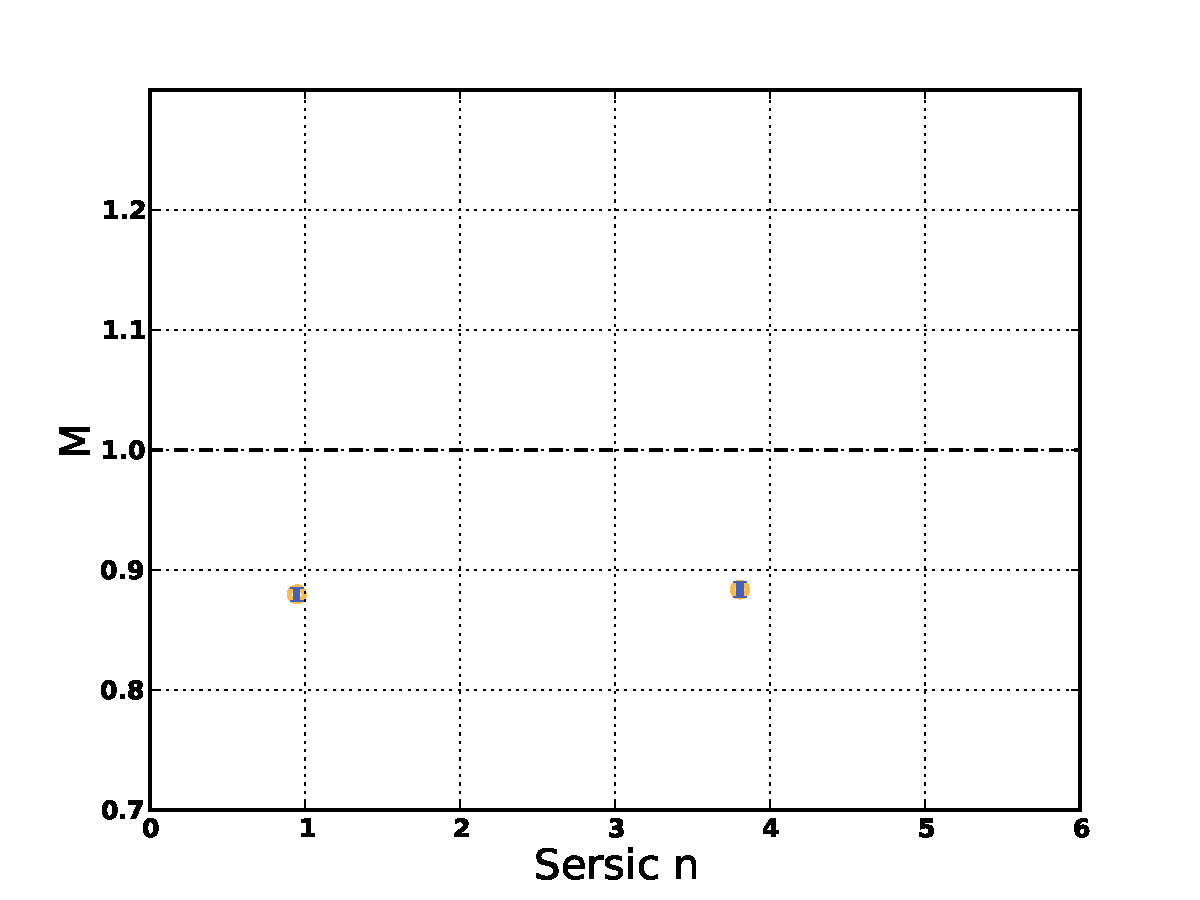
\includegraphics[width=0.45\textwidth]{fig/Mval_typeMJ.pdf} 
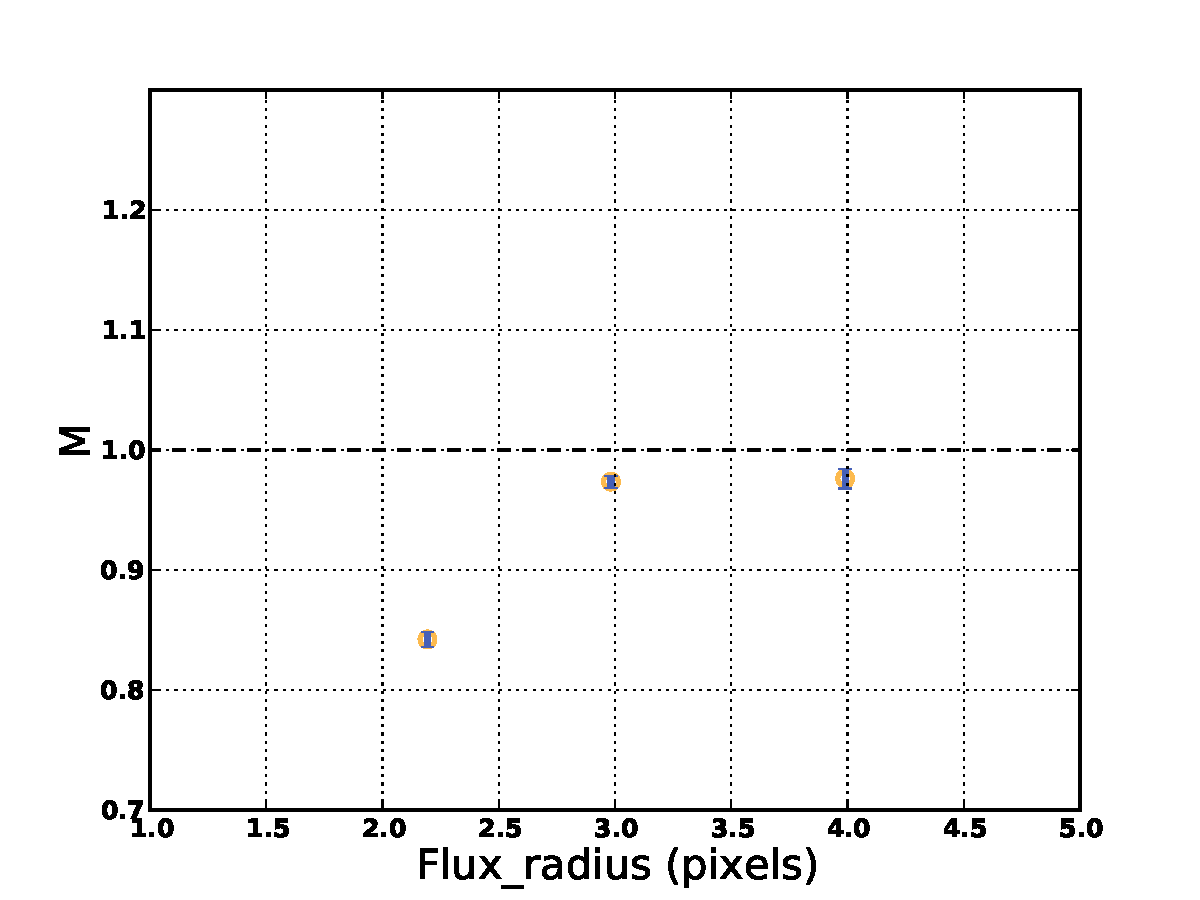
\includegraphics[width=0.45\textwidth]{fig/Mval_sizeMJ.pdf} 
\caption{The M and C values for ...}
\label{fig:DEIMOS_m}
\end{figure*}

\newpage 
\subsection{PFDNT}
For PFDNT we prepare time image postage stamp and PSF model in the
same way. Shear is estimated by applying roundness tests on the
anti-sheared, deconvolved Fourier transform of the image. To this end,
we use a weight function limited to frequencies where the Fourier
transform of the PSF is above zero according to Bernstein (2010). We
use the ellipticity estimate from the PKSB pipeline as a starting
point and sample ellipticities on a hexagonal grid to find the shear
estimate as the probability-weighted integral over ellipticity
space. \\

\begin{figure*}
\centering
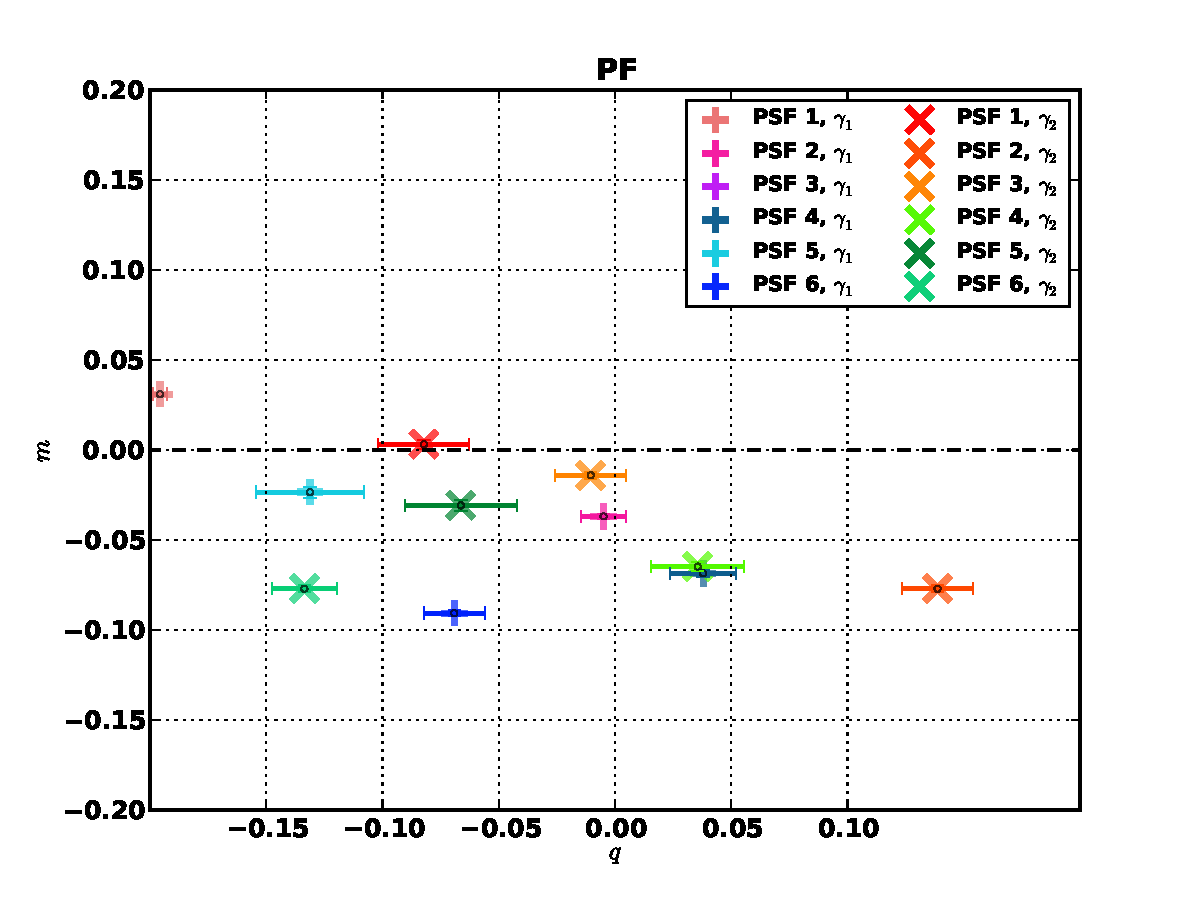
\includegraphics[width=0.45\textwidth]{fig/QMC_main_PF_f.pdf} 
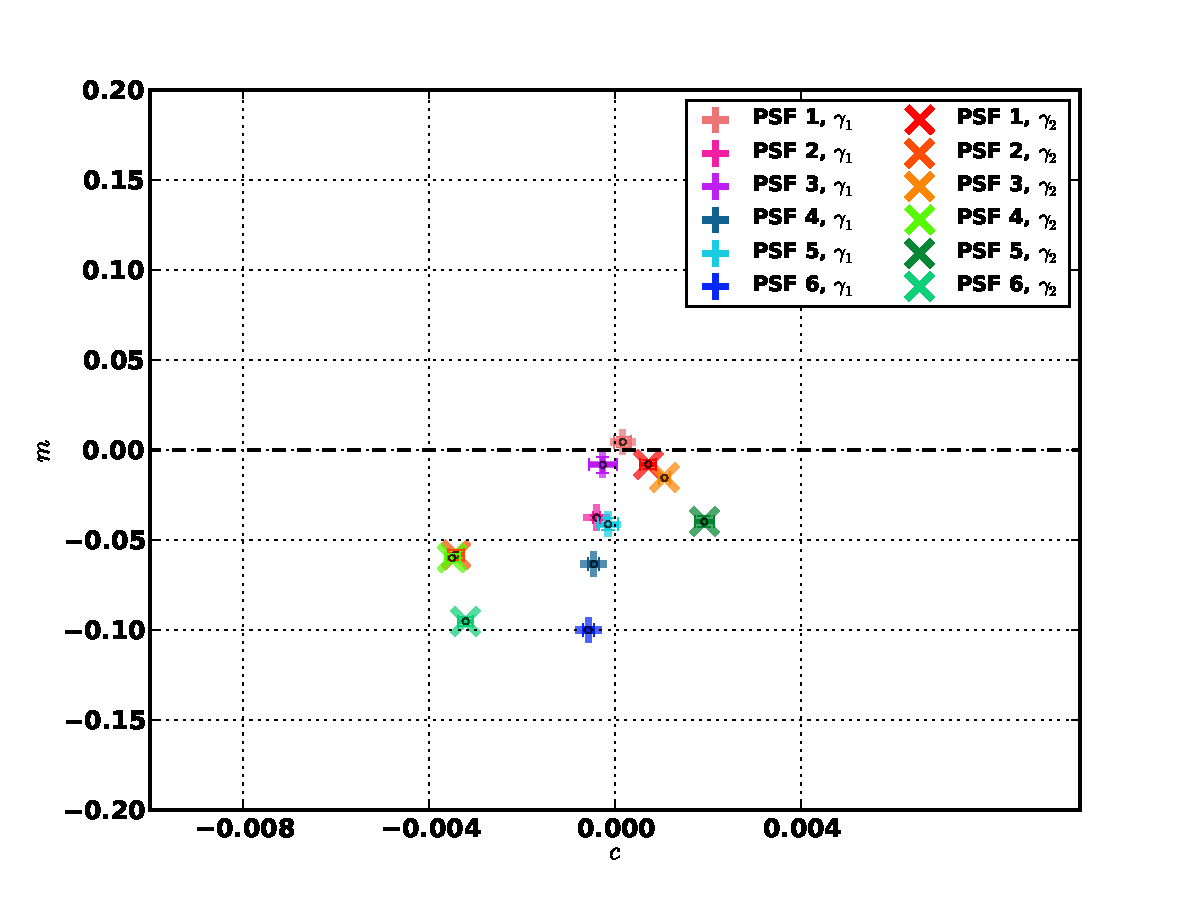
\includegraphics[width=0.45\textwidth]{fig/MC_main_PF_f.pdf} 
\caption{Average Q and M results for all pipelines for objects 
SNR $>$ 20 on the left and M and C results for all pipelines for objects 
SNR $>$ 20 on the right seperate by $\gamma_{1} $ and $\gamma_{2} $ as
well as PSF.}
\label{fig:PFDNT_qmc}
\end{figure*}
\begin{figure*}
\centering
\includegraphics[width=0.45\textwidth]{fig/MvalePF.pdf} 
\includegraphics[width=0.45\textwidth]{fig/Mval_typePF.pdf} 
\includegraphics[width=0.45\textwidth]{fig/Mval_sizePF.pdf} 
\caption{The M and C values for ...}
\label{fig:DEIMOS_m}
\end{figure*}

\clearpage

\section{Stacked weak lensing error}\label{App:statsec_a}
This section of the appendix contains information about the expected
statistical errors for a simulated cluster distribution of the stacked
weak lensing signal of DES.

\begin{figure*}
 \centering  % this centres figure in column
  \includegraphics[width=0.55\textwidth]{fig/M_NFW_2.pdf} 
  \includegraphics[width=0.55\textwidth]{fig/M_NFW_3.pdf} 
  \includegraphics[width=0.55\textwidth]{fig/M_NFW_4.pdf} 
  \caption{NFW mass and concentration measured on a reduced shear
    profile effected by shape measurement bias
   as measured on all images for galaxy objects with SNR $>$ 20.}
\label{fig:M_NFW_2}
\end{figure*} 


\begin{table*}
        \centering
        \begin{tabular}{|c|c|c|c|c|c|}  
          \hline
          N  &  $Z_{lens}$ & $Z_{source}$  & C & $M_{200m}$ $ M_\odot
          h^{-1}$  & $\Delta$ ln$(M)$ \\ 
          \hline
          228  & 0.16  & 0.58  & 5.58  & 2.91  & 0.039   \\
          \hline
          528  & 0.25  & 0.62  & 5.12  & 2.89  & 0.032   \\
          \hline
          776  & 0.35  & 0.66  & 4.73  & 2.78  & 0.037   \\
          \hline
          990  & 0.45  & 0.73  & 4.40  & 2.77  & 0.045   \\
          \hline
          986  & 0.55  & 0.79  & 4.12  & 2.71  & 0.069   \\
          \hline
          916  & 0.65  & 0.87  & 3.89  & 2.65  & 0.110   \\
          \hline
         54  & 0.16  & 0.58  & 5.31  & 5.67  & 0.060  \\
         \hline
         109  & 0.26  & 0.62  & 4.84  & 5.55  & 0.051   \\
         \hline
         120  & 0.35  & 0.66  & 4.49  & 5.53  & 0.063   \\
         \hline
         150  & 0.45  & 0.73  & 4.13  & 5.28  & 0.077   \\
         \hline
         138  & 0.55  & 0.79  & 3.93  & 5.20  & 0.121   \\
         \hline
         121  & 0.65  & 0.87  & 3.70  & 5.13  & 0.197  \\
          \hline
          5  & 0.17  & 0.58  & 4.93  & 11.85  & 0.161   \\
          \hline
          10  & 0.26  & 0.62  & 4.60  & 10.58  & 0.131   \\
          \hline
          14  & 0.36  & 0.66  & 4.22  & 11.12  & 0.134   \\
          \hline
          16  & 0.46  & 0.73  & 3.95  & 10.18  & 0.160   \\
          \hline
          13  & 0.54  & 0.79  & 3.74  & 9.94  & 0.264   \\
          \hline
          8  & 0.65  & 0.87  & 3.50  & 10.16  & 0.492   \\
          \hline
        \end{tabular}
        \caption{ The expected statistical error due to one method of
          cluster stacking for a DES like cluster distribution).}
    \label{table:NWF_4_b}
\end{table*}

\label{lastpage}
\end{document}
